% Options for packages loaded elsewhere
\PassOptionsToPackage{unicode}{hyperref}
\PassOptionsToPackage{hyphens}{url}
%
\documentclass[
]{book}
\usepackage{amsmath,amssymb}
\usepackage{iftex}
\ifPDFTeX
  \usepackage[T1]{fontenc}
  \usepackage[utf8]{inputenc}
  \usepackage{textcomp} % provide euro and other symbols
\else % if luatex or xetex
  \usepackage{unicode-math} % this also loads fontspec
  \defaultfontfeatures{Scale=MatchLowercase}
  \defaultfontfeatures[\rmfamily]{Ligatures=TeX,Scale=1}
\fi
\usepackage{lmodern}
\ifPDFTeX\else
  % xetex/luatex font selection
\fi
% Use upquote if available, for straight quotes in verbatim environments
\IfFileExists{upquote.sty}{\usepackage{upquote}}{}
\IfFileExists{microtype.sty}{% use microtype if available
  \usepackage[]{microtype}
  \UseMicrotypeSet[protrusion]{basicmath} % disable protrusion for tt fonts
}{}
\makeatletter
\@ifundefined{KOMAClassName}{% if non-KOMA class
  \IfFileExists{parskip.sty}{%
    \usepackage{parskip}
  }{% else
    \setlength{\parindent}{0pt}
    \setlength{\parskip}{6pt plus 2pt minus 1pt}}
}{% if KOMA class
  \KOMAoptions{parskip=half}}
\makeatother
\usepackage{xcolor}
\usepackage{longtable,booktabs,array}
\usepackage{calc} % for calculating minipage widths
% Correct order of tables after \paragraph or \subparagraph
\usepackage{etoolbox}
\makeatletter
\patchcmd\longtable{\par}{\if@noskipsec\mbox{}\fi\par}{}{}
\makeatother
% Allow footnotes in longtable head/foot
\IfFileExists{footnotehyper.sty}{\usepackage{footnotehyper}}{\usepackage{footnote}}
\makesavenoteenv{longtable}
\usepackage{graphicx}
\makeatletter
\def\maxwidth{\ifdim\Gin@nat@width>\linewidth\linewidth\else\Gin@nat@width\fi}
\def\maxheight{\ifdim\Gin@nat@height>\textheight\textheight\else\Gin@nat@height\fi}
\makeatother
% Scale images if necessary, so that they will not overflow the page
% margins by default, and it is still possible to overwrite the defaults
% using explicit options in \includegraphics[width, height, ...]{}
\setkeys{Gin}{width=\maxwidth,height=\maxheight,keepaspectratio}
% Set default figure placement to htbp
\makeatletter
\def\fps@figure{htbp}
\makeatother
\ifLuaTeX
  \usepackage{luacolor}
  \usepackage[soul]{lua-ul}
\else
  \usepackage{soul}
\fi
\setlength{\emergencystretch}{3em} % prevent overfull lines
\providecommand{\tightlist}{%
  \setlength{\itemsep}{0pt}\setlength{\parskip}{0pt}}
\setcounter{secnumdepth}{5}
\usepackage{booktabs}
\usepackage{amsthm}
\usepackage{LectureNoteMacro}
\usepackage{actuarialangle}
\usepackage{bbm}
\usepackage{mathtools}
\makeatletter
\def\thm@space@setup{%
  \thm@preskip=8pt plus 2pt minus 4pt
  \thm@postskip=\thm@preskip
}
\makeatother
\ifLuaTeX
  \usepackage{selnolig}  % disable illegal ligatures
\fi
\usepackage[]{natbib}
\bibliographystyle{apalike}
\usepackage{bookmark}
\IfFileExists{xurl.sty}{\usepackage{xurl}}{} % add URL line breaks if available
\urlstyle{same}
\hypersetup{
  pdftitle={SCMA266 Theory of Interest},
  pdfauthor={Pairote Satiracoo},
  hidelinks,
  pdfcreator={LaTeX via pandoc}}

\title{SCMA266 Theory of Interest}
\author{Pairote Satiracoo}
\date{2024-11-09}

\usepackage{amsthm}
\newtheorem{theorem}{Theorem}[chapter]
\newtheorem{lemma}{Lemma}[chapter]
\newtheorem{corollary}{Corollary}[chapter]
\newtheorem{proposition}{Proposition}[chapter]
\newtheorem{conjecture}{Conjecture}[chapter]
\theoremstyle{definition}
\newtheorem{definition}{Definition}[chapter]
\theoremstyle{definition}
\newtheorem{example}{Example}[chapter]
\theoremstyle{definition}
\newtheorem{exercise}{Exercise}[chapter]
\theoremstyle{definition}
\newtheorem{hypothesis}{Hypothesis}[chapter]
\theoremstyle{remark}
\newtheorem*{remark}{Remark}
\newtheorem*{solution}{Solution}
\begin{document}
\maketitle

{
\setcounter{tocdepth}{1}
\tableofcontents
}
\chapter{Cashflows, Interest and the Time Value of Money}\label{cashflows-interest-and-the-time-value-of-money}

\section{Introduction to Financial Modelling}\label{introduction-to-financial-modelling}

A financial model is a financial representation of a real world
financial situation, which is either a mathematical or statistical model
that describes the relationship among the variables of the financial
problem. Here are some types of financial models.

\begin{itemize}
\tightlist
\item
  \textbf{Financial statement model:} A financial statement model is a structured representation of a company's financial information, typically presented in a standardized format such as an Excel spreadsheet. This model includes projections of the company's income statement, balance sheet, and cash flow statement. It helps analysts, investors, and managers understand and evaluate a company's financial performance, growth prospects, and overall health by forecasting how various financial metrics will evolve over time based on assumptions about revenue, expenses, and other relevant factors. (see
  \url{https://corporatefinanceinstitute.com/resources/knowledge/accounting/three-financial-statements/})
\end{itemize}

\begin{itemize}
\tightlist
\item
  \textbf{Project finance models:} A project finance model is like a financial plan for a specific project, like long-term infrastructure, industrial projects, and public services. It lays out all the costs involved, such as construction, equipment, and operating expenses, and also predicts the future cash flows the project will generate, like revenue from selling electricity or tolls from the highway.
\end{itemize}

For instance, if a company wants to build a wind farm, the project finance model would estimate the costs of buying and installing wind turbines, as well as the income from selling the generated electricity over several years.

The model incorporates two main elements
of the project including loans and debt repayment. It can be used to
assess the risk-reward of lending to or investing in a long-term
project, i.e.~it can be used to tell whether the project has enough
cash to cover the debt in the long term. (see
\url{https://www.wallstreetprep.com/knowledge/project-finance-model-structure/})

\begin{itemize}
\item
  \textbf{Discounted cashflow model:} It is the model to
  estimate the value of an investment or business based on the present value of its future cash flows. It involves forecasting the cash flows the investment is expected to generate over time and then discounting those cash flows back to their present value using a chosen discount rate. By doing so, the model accounts for the time value of money, providing insight into whether the investment is overvalued or undervalued.
  (see
  \url{https://corporatefinanceinstitute.com/resources/templates/excel-modeling/dcf-model-template/})
\item
  \textbf{Pricing models:} The pricing model is a structured approach used to determine the appropriate price for a product or service. It considers various factors such as production costs, market demand, competition, and desired profit margins to arrive at a pricing strategy. The goal is to find a balance between attracting customers and generating sufficient revenue to ensure the business's sustainability and profitability.
\end{itemize}

This chapter covers the basic concepts of calculating interest,
including simple and compound interest, the frequency of compounding,
the effective interest rate and the discount rate, and the present and
future values of a single payment.

\section{Cashflows}\label{cashflows}

Cashflows are amounts of money which are received (or income, positive
cashflows) or paid (or outgo, negative cashflows) at particular times.
Those payments arise from a financial transaction, e.g

\begin{itemize}
\item
  a bank account,
\item
  a loan,
\item
  an equity,
\item
  a zero-coupon bond: A bond is a fixed income instrument that
  represents a loan from an investor to a debtor either a government
  or a corporation. A zero-coupon bond is a bond that pays no interest
  during its life.
\item
  a fixed interest security: A fixed-income security is a debt
  instrument such as a bond or debenture that investors use to lend
  money to a company in exchange for interest payments.
\item
  an index-linked security: An index-linked bonds pay interest that is
  tied to an underlying index, such as the consumer price index (CPI).
  Index-linked bonds are issued by governments to mitigate the effects
  of inflation by paying a real return plus accrued inflation.
\item
  an annuity: An annuity is a series of payments made at regular
  intervals, such as equal monthly payments on a mortgage.
\item
  a capital project etc.
\end{itemize}

Cash received represents inflows, income or also called \textbf{positive
cashflows}, while money spent represents outflows, outgo or \textbf{negative
cashflows}. The net cashflow at a given point in time is the difference
between expenses and income.

\begin{example}

\emph{A series of payments into and out of a bank account is given as
follows:}

\begin{itemize}
\item
  \emph{payments into the account : ฿1000 on 1 January 2014 and ฿100 on 1
  January 2016}
\item
  \emph{payments out of the account : ฿200 on 1 July 2015, ฿300 on 1 July
  2016, and ฿400 on 1 January 2018}
\end{itemize}

\end{example}

In practice, cashflows can be represented by a timeline as can be
illustrated in this example.

\begin{figure}

{\centering 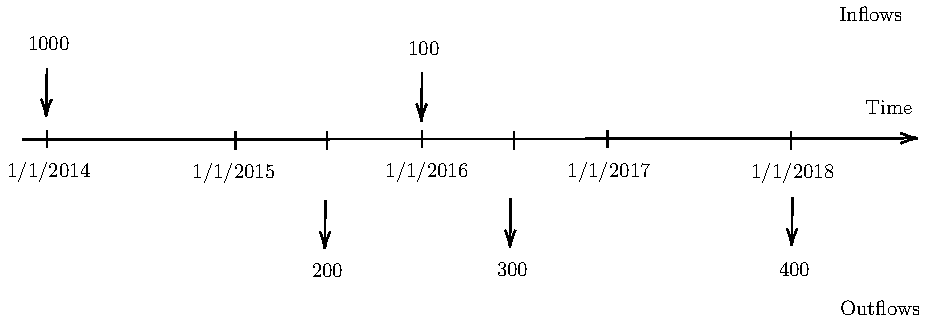
\includegraphics{SCMA266Bookdownproj_files/figure-latex/tikz-ex1-1} 

}

\caption{an example of a timeline}\label{fig:tikz-ex1}
\end{figure}

\section{Interest and the Time Value of Money}\label{interest-and-the-time-value-of-money}

This section introduces the time value of money using the concepts of
compound interest and discounting. The effect of interest rates on the
present value of future cash flows is discussed. The value of distant
cash flows in the present and current cash flows in the future are then
considered.

We illustrate the time value of money by considering the following
examples.

\begin{example}
\protect\hypertarget{exm:egpv}{}\label{exm:egpv}\emph{An investor want to make a payment of ฿10000 in 2 years. Suppose that a
bank pays compound interest at 4\% per annum effective. How much should
the initial investment?}
\end{example}

\textbf{Note} The amount we need to invest now (i.e.~the initial investment
in this example) is called the \emph{present value (PV)} or \emph{discounted
value} of the payments.

\textbf{Solution:} The interest for year 1 is

\[ X \cdot 0.04.\] For year 2 the principal is

\[ X + X \cdot 0.04 = X \cdot (1 + 0.04)\] so that the interest for the
year is

\[ X \cdot (1 + 0.04) \cdot 0.04.\]

By the end of 2 years an initial payment of ฿X will have accumulated to:

\[X\cdot (1 + 0.04) + X \cdot (1 + 0.04) \cdot 0.04 =   X  \cdot  1.04^2 = 10000.\]
Hence,

\[X = \frac{10000}{1.04^2} = 9245.56213,\]

\textbf{Note} We refer to the amount to which the capital accumulates with
the addition of interest as \emph{accumulation} or \emph{accumulated value}.

\begin{example}

\emph{Consider the following arguments}

\begin{itemize}
\item
  \emph{It is obvious that you would prefer to have ฿1100 now than ฿1000
  now.}
\item
  \emph{If we receive and hold ฿1 now, then it is worth more than receiving
  and holding ฿1 at some time in the future? Why is this?}
\item
  \emph{Is it obvious that your would be better off with ฿1100 in 2 years
  than ฿1000 now?}
\end{itemize}

\end{example}

\textbf{Solution:}

For the second argument, this one baht will grow to \(1 + r\) in the first
year, \((1 + r)^2\) in two years, and so on. These amounts are clearly
worth more than receiving and holding ฿1 at the same time in the future.

For the last argument, we need to compare the values of the amounts received at different times. To do this, we can look at the today's
values of ฿1100 received in 2 years assuming that we can invest at an
annual interest rate of \(r\) percent.

The present value of this amount \(X\) in year 2 is \[ 1100/(1 + r)^2.\] Assuming \(r = 5\%\), the present value of \(X\) is 997.7324263.

Comparing the values in today's baths, it is better to
have ฿1000 now than to have ฿1100 in 2 years.

\textbf{Notes} From the above example,

\begin{enumerate}
\def\labelenumi{\arabic{enumi}.}
\item
  One can deposit or invest ฿1 now and will receive ฿1 back and a
  reward called \emph{interest} at some point in the future. Because of its
  potential earning power, money in the present is worth more than an
  equal amount in the future. This is a fundamental financial
  principle known as \textbf{the time value of money}.
\item
  At a given point of time, cash has a monetary value, but also has a
  \emph{time value}.
\item
  The amount deposited or invested is called \emph{capital} or \emph{principal}.
\end{enumerate}

\subsection{Simple interest}\label{simple-interest}

Simple interest is a calculation of interest that does not take into
account the effect of compounding. Under simple interest, the amount of interest that accrues over time is proportional to the length of the period.

Suppose an amount \(C\) is deposited in
an account that pays simple interest at the rate of \(i\)\% per annum. Then
after \(n\) years the deposit will have accumulated to
\[C( 1 + i \cdot n).\] Hence, the interest accrued over \(n\) years is
\[\text{Simple Interest}  = C \cdot i \cdot n.\]

\textbf{Note} Auto loans and short-term personal loans are usually simple
interest loans.

\begin{example}

\emph{An investor deposits ฿10000 in a bank account that pays simple interest
at a rate of 5\% per annum. Calculate}

\begin{enumerate}
\def\labelenumi{\arabic{enumi}.}
\item
  \emph{interest he will earn after the first two years.}
\item
  \emph{interest he will earn after the first three months.}
\end{enumerate}

\end{example}

\textbf{Note} When \(n\) is not an integer, interest is paid on a pro-rate
basis (in proportion).

\textbf{Solution:}

\begin{enumerate}
\def\labelenumi{\arabic{enumi}.}
\item
  At the end of 2 years the interest earned is
  \[10000 \cdot 0.05 \cdot 2 = 1000.\]
\item
  At the end of 3 months the interest earned is
  \[10000 \cdot 0.05 \cdot \frac{3}{12} = 125.\] Alternatively, the
  interest per month is 5\%/12 = 0.4167\% and hence the interest earned
  can be calculated as \[10000 \cdot 0.004167 \cdot 3 = 125.\]
\end{enumerate}

\subsection{Compound interest}\label{compound-interest}

In compound interest, the accumulated amount over a period of time is the capital of the following period. Therefore, a capital of 1 unit at the end of the year increases to \(1 + i\) units, which becomes the capital for the following year.

For year 2, the principal is \(1 + i\) and the interest for the year is
\(( 1 + i ) \cdot i\). By the end of 2 years, an initial payment of 1 will have accumuulated to
\[ (1+i) + ( 1 + i ) \cdot i = (1+i)^2.\]

As this progression continues, the accumulated amount of \(X\) units at the end of year \(n\) becomes
\[ X\cdot(1 + i)^n. \]

\theNote In this case, we can take money out and reinvest it as new capital illustrated in the timeline.

\begin{figure}

{\centering 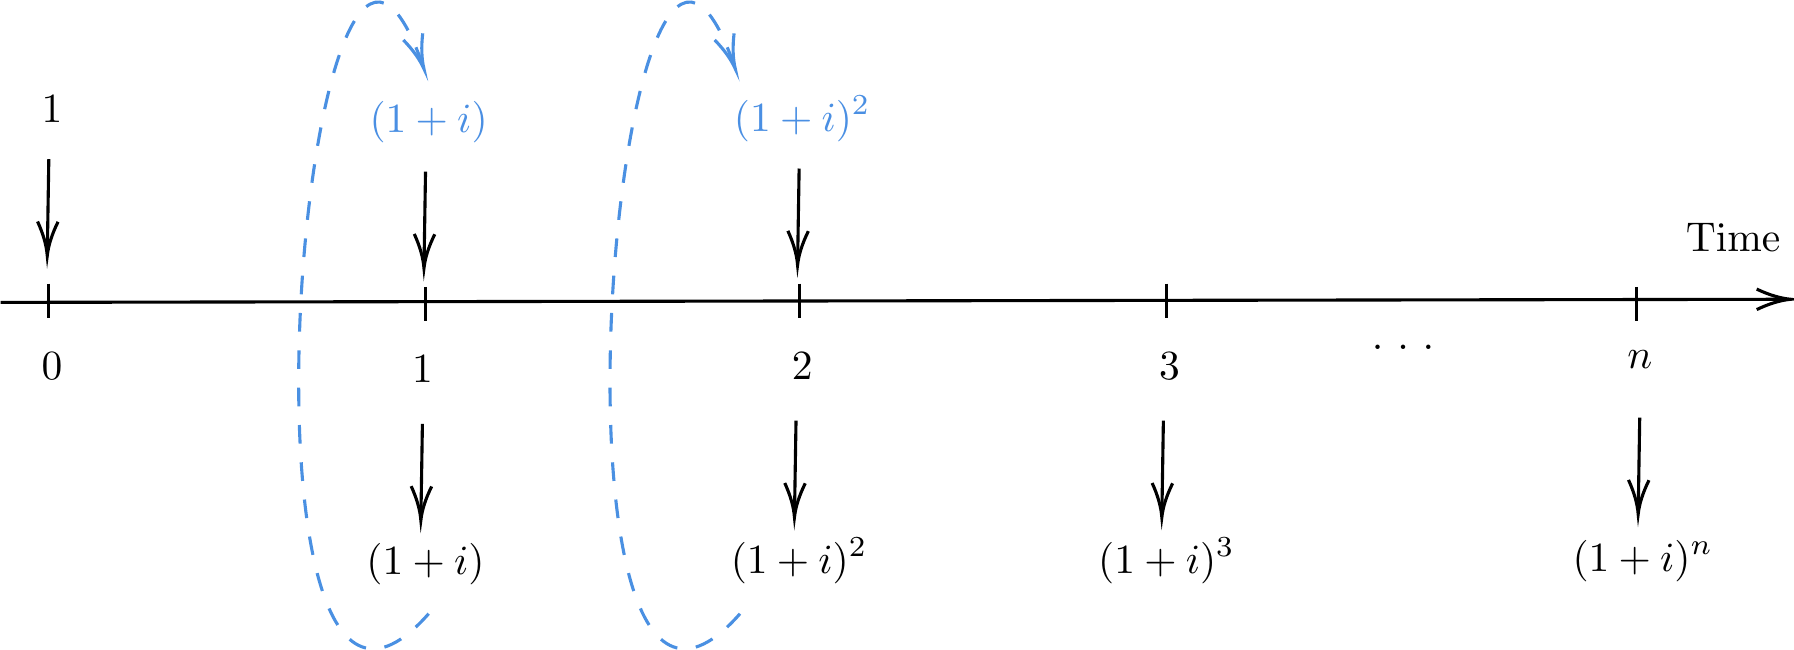
\includegraphics{SCMA266Bookdownproj_files/figure-latex/tikz-ex2-1} 

}

\caption{a timeline of compounding interest}\label{fig:tikz-ex2}
\end{figure}

\begin{exercise}
(Excel) Use Excel to create a table showing the accumulated amounts at the end of each year for 15 years for a principal of ฿100 under the simple interest approach and the compound interest approach with \(r = 6\%\) for both cases.
Discuss the results obtained (How long does it take to double the investment? How much will the principal grow over a 15-year period?)
\end{exercise}

The effect of compounding is to increase the total amount of accumulation. The effect is greater when the interest rate is high. This example shows two examples of the accumulated amount of ฿100 under the simple interest approach and the compound interest approach. As can be seen, the compound interest method makes the principle increase much faster than the simple interest method when the interest rate is high.

\section{Frequency of Compounding}\label{frequency-of-compounding}

Even though the interest rate is typically expressed in annual terms, an investment's interest is frequently paid more frequently than once per year. For example, a savings account may offer an interest rate of 4\% per year, credited quarterly. This interest rate is usually referred to as \textbf{nominal rate of interest}, i.e., 4\% due four times per year.

We will see that the frequency of interest payments, also known as the frequency of compounding, has a significant impact on the total amount accrued and the interest collected. Consequently, it is crucial to precisely specify the rate of interest.

We use \(i^{(m)}\) to represent the nominal rate of interest payable \(m\) times a year in order to underline the significance of the frequency of compounding. Therefore, \(m\) is the
frequency of compounding per year and \(1/m\) year is the \textbf{compounding period} or \textbf{conversion period}.

\textbf{Note} The nominal rate of interest payable \(m\) times per period is also known as the rate of interest convertible \(m\)thly or compounded \(m\)thly.

\begin{example}
Calculate the accumulated value in 1 year of a deposit of ฿100 in a saving account that earns interest at 10\% payable quarterly.
\end{example}

\textbf{Solution:} In this example, the nominal rate of interest of \(i^{(4)} = 10\%\) p.a. convertible
quarterly means an interest rate of 10\%/4 = 2.5\% per quarter. In this case, the interest rate of 2.5\% is called \emph{effective interest}. The effective interest rate of \(i\) per unit of time (which may be month, quarter, etc.) is the amount of interest received at the end of a unit of time per ฿1 invested at the beginning of that unit.

Therefore, the nominal interest rate \(i^{(4)} = 10\%\) is equivalent to an
\emph{effective interest rate} of \(2.5\%\) per quarter.
The accumulated value in
1 year is \(100 (1 + \frac{10\%}{4})^4 = 100 (1 + 2.5\%)^4 = 110.3813\).

Note that after compound interest is
taken into account, the interest income of an investor at the quarterly
convertible nominal interest rate of 10\% p.a. is 10.3813 (or 10.3813\%.p.a. effective)

\begin{example}
\emph{At a rate of 12\% p.a. effective, draw a timeline to show cashflows if
฿100 is invested at the start of the year.}
\end{example}

\textbf{Solution:} The accumulated value of ฿100 at the end of the year is
\(100 (1 + 12\%) = 112\).

\begin{example}
\emph{At a rate of 12\% p.a. compounding quarterly, draw a time line to show
cashflows if ฿100 is invested at the start of the year.}
\end{example}

\textbf{Solution:} The nominal interest rate \(i^{(4)} = 12\%\) is equivalent
to an effective interest rate of \(3\%\) per quarter. The accumulated
value in 1 year is \(100 (1 + 3\%)^4 = 112.55\). After compound interest
is taken into account, the interest income of an investor at the
quarterly convertible nominal interest rate of 10\% p.a. is 12.55 (or
12.55\%. p.a. effective)

\textbf{Note} \(i^{(m)}\) is a nominal rate of interest which is equivalent to \(i^{(m)}/m\) applied for
each \(m\)th of a period. The interest is paid \(m\) times per measurement period.

The value at time \(n\) can be considered as the \textbf{annuity} with a cashflow of \(i^{(m)}/m\) per period for \(n\) years together with the capital at time \(n\) as shown in the following figure.
Therefore, the accumulated value in 1 year can also be calculated as \(100( 1 + 0.03 s_{\angl{4}}^{3\%})\). The concept of annuity will be discussed in the subsequent section.

\begin{figure}

{\centering 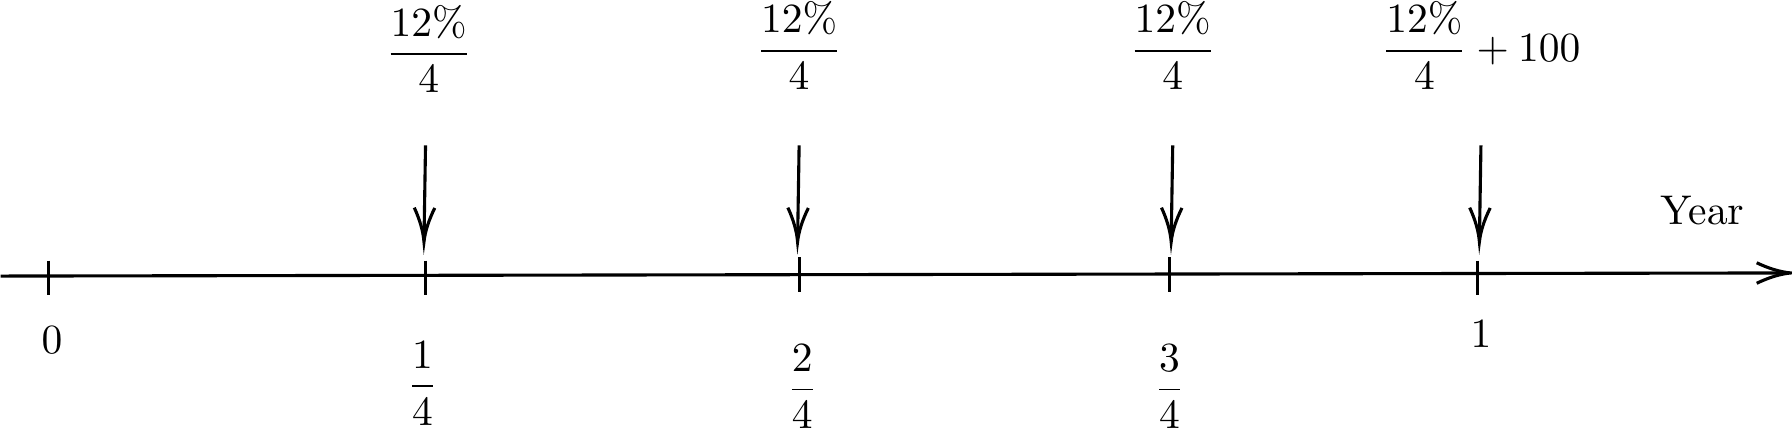
\includegraphics{SCMA266Bookdownproj_files/figure-latex/tikz-ex5-1} 

}

\caption{Frequency of Compouding vs Annuity}\label{fig:tikz-ex5}
\end{figure}

In general, we have

\begin{figure}

{\centering 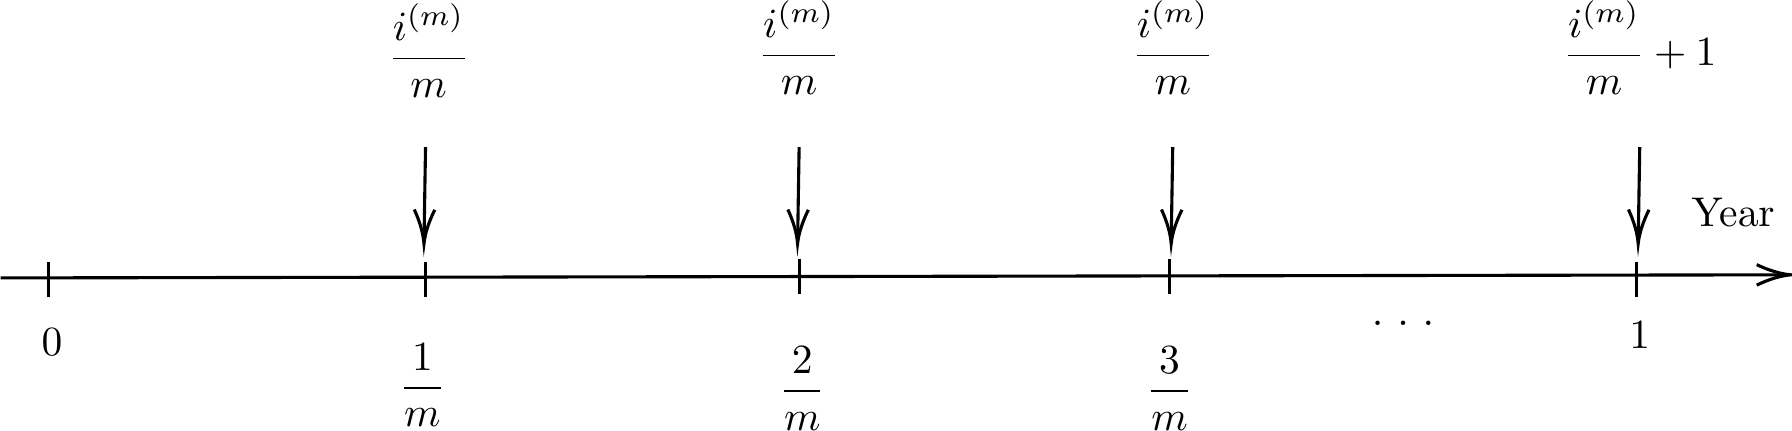
\includegraphics{SCMA266Bookdownproj_files/figure-latex/tikz-ex4-1} 

}

\caption{Frequency of Compouding vs Annuity}\label{fig:tikz-ex4}
\end{figure}

\subsection{Effective rate of interest}\label{effective-rate-of-interest}

The compounding frequency affects the accumulated amount. As a result, it may be inaccurate to compare two investment strategies only based on their nominal rates of return without also taking into account their frequency of compounding. It is necessary to compare different investment strategies on an equal basis. The measure known as the \textbf{effective interest rate} is often used for this purpose.

The effective rate of interest of \(i\) per time unit is the amount of
interest received at the end of one time unit per ฿1 invested at the
start of that time unit.

\begin{example}
\emph{An investor invests ฿1 at 7.5\% p.a. (per annum) effective. Then}
\(i = 0.075\). Calculate the value of investment after one year.
\end{example}

\textbf{Solution:} The value of investment after one year at this rate is
\[1 \times ( 1 + 0.075) = 1.075.\]
In particular, the amount of
interest received at the end of the year per ฿1 invested is 0.075.

\begin{example}
\emph{An investor invests ฿1000 at 5.25\% per half-year effective. Then}
\(i = 0.0525\). Calculate the value of investment after half a year.
\end{example}

\textbf{Solution:} The value of investment after half year at this rate is
\[1000 \times ( 1 + 0.0525) = 1052.5.\]
Again, the amount ofinterest received at the end of the quarter of ฿1 invested is 0.0525.

\textbf{Note} The time unit is an \textbf{essential part of the definition}.

\begin{example}
\emph{An investor invests ฿1 at effective rate} \(i\)\% per time unit for \(n\)
time units. Calculate the value of investment after two, three,
\(\ldots\), \(n\) time units.
\end{example}

\textbf{Note} Here we assume that we can take money out and reinvest it as
new capital (see the timeline).

\begin{center}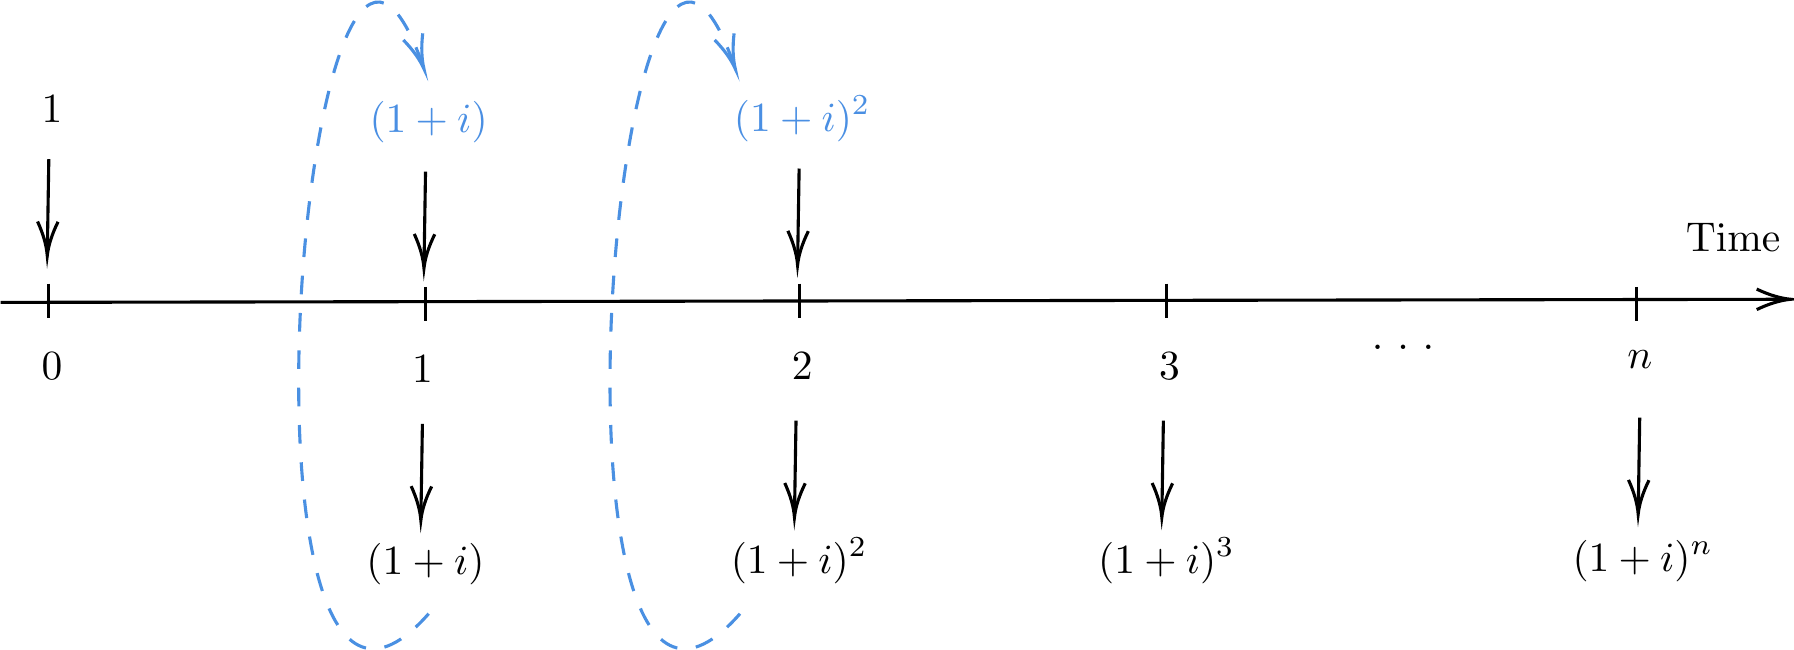
\includegraphics{SCMA266Bookdownproj_files/figure-latex/tikz-ex6-1} \end{center}

\begin{example}
\emph{An investor invests ฿200 at} \(3\)\% pa effective. What will be the
deposit have accumulated to after 5 years.
\end{example}

\textbf{Solution:} The deposit accumulates to
\(200 \cdot (1.03)^5 = 231.854815\) after 5 years.

\begin{example}

Consider the following problems.

\begin{enumerate}
\def\labelenumi{\arabic{enumi}.}
\item
  \emph{An investor invests ฿500 at} \(2.75\)\% per quarter effective. What
  will be the deposit have accumulated to after 9 months.
\item
  \emph{An investor invests ฿2000 at} \(6\)\% per half-year effective. What
  will be the deposit have accumulated to after 2 years.
\end{enumerate}

\end{example}

\textbf{Solution:}

\begin{enumerate}
\def\labelenumi{\arabic{enumi}.}
\item
  Accumulating the 500 for 9 months at this rate gives
  \[500 \cdot (1.0275)^3 = 542.394773.\]
\item
  After 2 years the accumulation is
  \[2000 \cdot (1.06)^4 = 2524.95392.\]
\end{enumerate}

\textbf{Notes}

\begin{enumerate}
\def\labelenumi{\arabic{enumi}.}
\item
  The model under the effective rate of interest condition is a
  model of \emph{compound interest}, where interest is earned on interest
  previously earned. Unless state otherwise, we shall assume that \(i\) is
  the compound interest rate.
\item
  In practice, it is easier to work with the effective rate of
  interest which is defined in a suitable time unit.
\end{enumerate}

The following formula can be used to convert between the effective rate
\(i\) p.a. and the nominal rate \(i^{(m)}\) p.a.:
\[( 1 + i) = \left( 1 + \frac{i^{(m)}}{m}\right)^m.\]

\begin{example}

Consider the following problems.

\begin{enumerate}
\def\labelenumi{\arabic{enumi}.}
\item
  \emph{Express a nominal annual interest rate of 9\% convertible
  half-yearly as a monthly effective interest.}
\item
  \emph{Express a two-monthly effective interest of 3\% as a nominal annual
  interest rate convertible two-monthly.}
\end{enumerate}

\end{example}

\textbf{Solution:}

\begin{enumerate}
\def\labelenumi{\arabic{enumi}.}
\item
  The effective rate \(i\)\% p.a. is \[i = ( 1 + \frac{0.09}{2})^2 - 1.\]
  Hence the monthly effective rate is
  \(j = (1 + i)^{1/12} - 1 = ( 1 + \frac{0.09}{2})^{2/12} - 1 = 0.007363\).
\item
  A nominal annual interest rate convertible two-monthly is
  \(6 \cdot 3\% = 18\%\).
\end{enumerate}

\begin{example}

\emph{Express each of the following effective rates per annum as a nominal
rate, and vice versa.}

\begin{longtable}[]{@{}ll@{}}
\toprule\noalign{}
\textbf{\emph{Effective Rate}} & \textbf{\emph{Nominal Rate}} \\
\midrule\noalign{}
\endhead
\bottomrule\noalign{}
\endlastfoot
\(i\) = 0.04 & \(i^{(4)} = 0.039412\) \\
\(i\) = 0.10 & \(i^{(12)} = 0.095690\) \\
\(i\) = 0.06152 & \(i^{(2)} = 0.06\) \\
\(i\) = 0.126825 & \(i^{(12)} = 0.12\) \\
\end{longtable}

\end{example}

\subsection{Compounding over any number of time units}\label{compounding-over-any-number-of-time-units}

Suppose an amount ฿1 is invested at the rate of \(i\)\% per time unit. At
time \(t\) the accumulation is \((1 + i)^t\).

\begin{example}
\leavevmode

\begin{enumerate}
\def\labelenumi{\arabic{enumi}.}
\item
  \emph{An investor invests ฿4000 at} \(8.5\)\% per quarter effective. What
  will be the deposit have accumulated to after 1 month.
\item
  \emph{An investor invests ฿800 at} \(6\)\% per half-year effective. What
  will be the deposit have accumulated to after 2.6 years.
\end{enumerate}

\end{example}

\textbf{Solution:}

\begin{enumerate}
\def\labelenumi{\arabic{enumi}.}
\item
  The accumulation after 1 month is
  \(4000 \cdot 1.085^{1/3} = 4110.265768.\)
\item
  The accumulation after 2.6 years is
  \(800 \cdot 1.06^{5.2} = 1083.129754.\)
\end{enumerate}

\begin{exercise}
(Excel) Use Excel to create a table showing the accumulated amounts after 1 year under several different compounding frequencies (yearly, quarterly, monthly, daily) for a principal of ฿100 under with nominal rate of \(r = 4\%\) per annum.

Discuss the results obtained. What happens if the compounding is made over infinitely small intervals (i.e.~as \(m \rightarrow \infty\))?
\end{exercise}

\subsection{Changing the time period of the effective rates of interest}\label{changing-the-time-period-of-the-effective-rates-of-interest}

It is often very useful to change the effective rate of interest per
time period to another. For example, if the effective rate of interest
is defined per annum but cashflows occur monthly.

Let \(i\) be the effective rate of interest per \(t_i\) years (which can be
any positive number, for e.g.~\(t_i = 1/2\)). Here \(t_i\) years can be
regarded as one time unit. Let \(j\) be the effective rate of interest per
\(t_j\) years.

\begin{example}
\emph{Find the condition under which the two effective rates of interest} \(i\)
and \(j\) are equivalent.
\end{example}

\textbf{Solution:} Suppose we invest 1 for one year. Then at the end of the
year under each rate of interest, we will have
\[(1+i)^{1/t_i} \text{ and } (1+j)^{1/t_j}.\] Two rates of interest are
equivalent if the given amount of principal invested for the same length
of time produces the same accumulated value, i.e.
\[(1+i)^{1/t_i} = (1+j)^{1/t_j}.\] Solving the equation for \(j\) yields
\[j = (1+i)^{t_j/t_i} - 1.\]

\begin{example}
\leavevmode

\begin{enumerate}
\def\labelenumi{\arabic{enumi}.}
\item
  \emph{If the effective rate of interest is 6\% per annum, what is the
  effective rate of interest per half-year?}
\item
  \emph{If the effective rate of interest is 12\% per two-years effective,
  what is the effective rate of interest per quarter-year?}
\item
  \emph{If the effective rate of interest is 2\% per month effective, what
  is the effective rate of interest per 1.5-years?}
\end{enumerate}

\end{example}

\textbf{Solution:}

\begin{enumerate}
\def\labelenumi{\arabic{enumi}.}
\item
  \(i = 6\%\) p.a. Then
  \[j = (1.06)^{1/2} -1 = 0.029563 \text{ per half-year}.\]
\item
  \(i = 12\%\) per two-years. Then
  \[j = (1.12)^{1/(2\times4)} -1 = 0.0142669 \text{ per quarter-year}.\]
\item
  \(i = 2\%\) per month. Then
  \[j = (1.02)^{1.5/(1/12)} -1 = 0.428246 \text{ per 1.5-years}.\]
\end{enumerate}

\subsection{Non-constant interest rates}\label{non-constant-interest-rates}

The effective rate may not be the same during every time period. We
shall assume that the rates in every future time periods are known in
advance.

\begin{example}

\emph{The effective rate of interest per annum was 4\% during 2015, 4.5\%
during 2016 and 5\% during 2017. Calculate the accumulation of ฿200
invested on}

\begin{enumerate}
\def\labelenumi{\arabic{enumi}.}
\item
  \emph{01/01/2015 for 3 years}
\item
  \emph{01/07/2015 for 2 years}
\item
  \emph{01/04/2016 for 1.5 years}
\end{enumerate}

\end{example}

\textbf{Solution:}

\begin{enumerate}
\def\labelenumi{\arabic{enumi}.}
\item
  Accumulating the ฿200 for the first year at the rate of 4\% p.a.
  gives \[200 \cdot 1.04.\] The accumulated value was then invested at
  the rate of 4.5\% p.a. for another year, and its value at after 2
  years was \[200 \cdot 1.04 \cdot 1.045.\] At the rate of 5\% in the
  final year, the value after 3 years was
  \[200 \cdot 1.04 \cdot 1.045 \cdot 1.05 = 228.228.\]
\item
  The accumulation is
  \[200 \cdot 1.04^{1/2} \cdot 1.045 \cdot 1.05^{1/2} = 218.4025.\]
\item
  The accumulation is
  \[200 \cdot 1.045^{9/12} \cdot 1.05^{3/4} = 214.416986.\]
\end{enumerate}

\subsection{Accumulation factors}\label{accumulation-factors}

Let \(i\) be the effective rate of interest per one time unit and \(s < t\).
We define

\begin{itemize}
\item
  the accumulation factor per one time unit \[A(0,1) = (1 + i).\]
\item
  the accumulation factor per \(t\) time units \[A(0,t) = (1 + i)^t.\]
\item
  the accumulation factor at time \(t\) of 1 unit invested at time \(s\)
  \[A(s,t).\]
\end{itemize}

\begin{example}

\emph{The effective rate of interest per annum was 6\% during 2015, 8\% during
2016 and 10\% during 2017. Calculate the following accumulation factors.}

\begin{enumerate}
\def\labelenumi{\arabic{enumi}.}
\item
  \(A(01/01/15, 01/01/18),\) i.e.~the accumulation at 01/01/18 of an
  investent of 1 at 01/01/15
\item
  \(A(01/07/15, 01/07/17)\)
\item
  \(A(01/04/16, 01/10/17)\)
\end{enumerate}

\end{example}

\textbf{Solution:}

\begin{enumerate}
\def\labelenumi{\arabic{enumi}.}
\item
  \(A(01/01/15, 01/01/18) = (1.06)(1.08)(1.1) = 1.25928\)
\item
  \(A(01/07/15, 01/07/17) = (1.06)^{1/2}(1.08)(1.1)^{1/2} = 1.166200\)
\item
  \(A(01/04/16, 01/10/17) = (1.08)^{3/4}(1.1)^{3/4} = 1.137922\)
\end{enumerate}

\subsection{Present values and discount factors}\label{present-values-and-discount-factors}

Recall from Example \ref{exm:egpv} that the amount
\(\displaystyle{\frac{10000}{1.04^2}}\) we need to invest now to obtain
฿10000 in two years is called the \emph{present value (PV)} or \emph{discounted
value} of the payments.

We define the discount factor \(v\) per annum, at rate \(i\) p.a. effective
to be the present value of a payment of 1 due in 1 year?s time, i.e.
\[v = \frac{1}{1+i}.\]

\begin{example}
\emph{Calculate the present of ฿25000 due in 3 years at an effective rate of
interest of 6\% per annum.}
\end{example}

\textbf{Solution:} The present value is
\[25000 \cdot \frac{1}{1.06^3} = 20990.482076.\] It is the discounted
value of 25000 due in 3 years.

\begin{example}
\emph{How much should we invest now to meet a liability of ฿50000 in 5 years
at an effective rate of interest of 3\% per half-year.}
\end{example}

\textbf{Solution:} The amount we need to invest now to meet the future
liability of 50000 in 5 years is the present value
\[50000 \cdot \frac{1}{1.03^{10}} = 37204.695745.\]

\textbf{Note} It follows that the \(PV\) of ฿1 in \(t\) time units at \(i\)
effective rate of interest per time unit is
\[PV = \frac{1}{(1+i)^t} = v^t.\]

\begin{example}

\emph{Given the discount factor per year} \(v = 0.9\), calculate

\begin{enumerate}
\def\labelenumi{\arabic{enumi}.}
\item
  \emph{the effective rate of interest per year.}
\item
  \emph{the equivalent discount factor per half-year.}
\end{enumerate}

\end{example}

\textbf{Solution:}

\begin{enumerate}
\def\labelenumi{\arabic{enumi}.}
\item
  From \(\displaystyle{ v= \frac{1}{1+i} = 0.9}\), solving the equation
  for \(i\) gives \[i = \frac{1}{v} - 1 = 0.111111 \text{ per year}.\]
\item
  Let \(j\) be the effective rate of interest per half-year. Then
  \[j = (1+ i)^{1/2} -1 = 0.054093.\] Then, the discount factor per
  half-year is \[v = \frac{1}{1+j} = \frac{1}{1.054093} = 0.948683.\]
\end{enumerate}

Similarly, we define

\begin{itemize}
\item
  the discount factor per one time unit \[V(0,1) = 1/(1 + i).\]
\item
  the discount factor per \(t\) time units \[V(0,t) = 1/(1 + i)^t.\]
\item
  for \(s < t\), the discount factor at time \(s\) of 1 unit receivable at
  time \(t\) \[V(s,t) =  (1 + i)^{s - t}.\]
\end{itemize}

\textbf{Notes}

\begin{enumerate}
\def\labelenumi{\arabic{enumi}.}
\item
  \(V(s,t) = A(s,t)^{-1}\)
\item
  For \(r < s < t\), the following holds:

  \begin{itemize}
  \item
    \(A(r,t) = A(r,s) A(s,t)\)
  \item
    \(V(r,t) = V(r,s) V(s,t)\)
  \end{itemize}
\end{enumerate}

\section{Cashflows and Annuities}\label{cashflows-and-annuities}

Consider a series of cashflows defined by (see the timeline)

\begin{enumerate}
\def\labelenumi{\arabic{enumi}.}
\item
  the times of payments (cashflows), denoted by \(t_1, t_2, \ldots,\)
  and
\item
  the amount of payments, denoted by \(C_{r}\) (or \(C_{t_r}\)), which
  will be paid at time \(t_r\), for \(r = 1,2, \ldots\). The amounts can
  be positive or negative
\end{enumerate}

The present value at any time \(t\) of this series of cashflow is
\[PV(t) = \sum_{r=1}^\infty C_r (1 + i)^{t - t_r} = \sum_{r=1}^\infty C_r v^{t _r - t}\]
where \(i\) is the effective rate of interest.

The above formula can be obtained by summing these two components:

\begin{itemize}
\item
  for all \(t_r < t\), adding up the accumulations of these individual
  cashflows up to time \(t\), and
\item
  for all \(t_r > t\) , adding up the discounted values of these
  individual cashflows back to time \(t\).
\end{itemize}

\begin{center}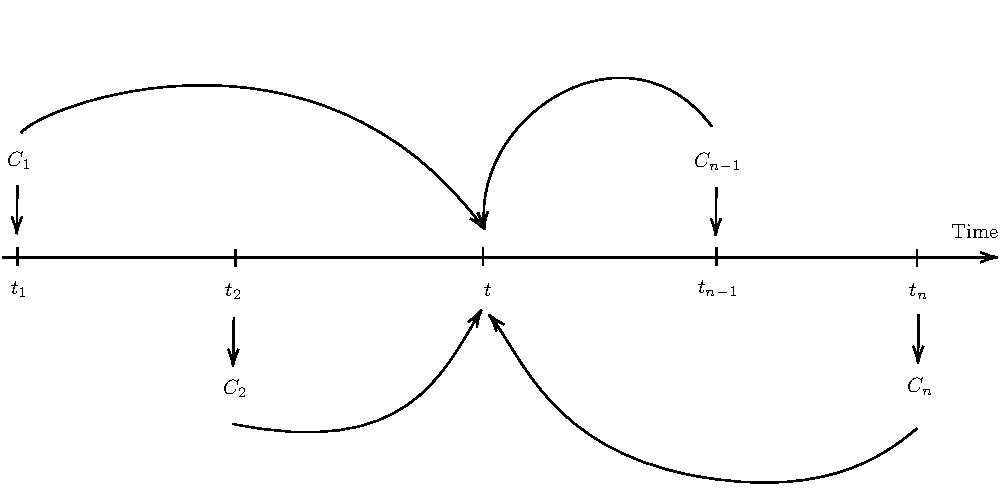
\includegraphics{SCMA266Bookdownproj_files/figure-latex/tikz-ex7-1} \end{center}

\textbf{Notes}

\begin{enumerate}
\def\labelenumi{\arabic{enumi}.}
\item
  At a fixed effective rate of interest, the original series of
  cashflows is equivalent to a single payment of amount \(PV(t)\) at
  time \(t\).
\item
  If two different series of cashflows have the same \(PV\) at one time
  at a given effective rate of interest, then they have the same \(PV\)
  at any time at that effective rate of interest.
\end{enumerate}

\begin{example}

\emph{Let} \(i = 4\%\) effective per time unit. Cashflows are given as follows:

\begin{itemize}
\item
  \(C_1 = 200\) at time \(t_1 = 1\).
\item
  \(C_2 = 300\) at time \(t_2 = 3\).
\item
  \(C_3 = -100\) at time \(t_3 = 5\).
\item
  \(C_4 = -50\) at time \(t_4 = 6\).
\end{itemize}

\emph{Calculate}

\begin{enumerate}
\def\labelenumi{\arabic{enumi}.}
\item
  \emph{the accumulation at time} \(t = 7\).
\item
  \emph{the present value at time} \(t = 0\).
\item
  \emph{the present value at time} \(t = 4\).
\end{enumerate}

\end{example}

\textbf{Solution:}

\begin{center}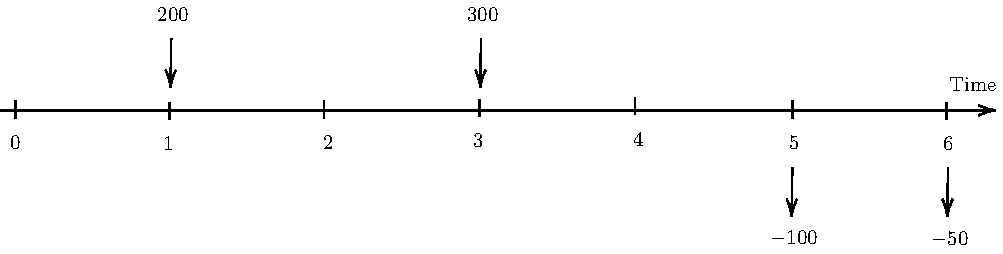
\includegraphics{SCMA266Bookdownproj_files/figure-latex/tikz-ex8-1} \end{center}

\begin{enumerate}
\def\labelenumi{\arabic{enumi}.}
\item
  The series of cashflows is shown in the following timeline. The
  accumulation at time \(t = 7\) is \[\begin{aligned}
      \sum_{r=1}^4 A(t_r,7) &= 200 \cdot A(1,7) +  300 \cdot A(3,7) -  100 \cdot A(5,7) -  50 \cdot A(6,7) \\
      &= 200 \cdot 1.04^6 + 300 \cdot 1.04^4 - 100 \cdot 1.04^2 - 50 \cdot 1.04 \\
      & = 443.861372\end{aligned}\]
\item
  The present value at time \(t = 0\) can be obtained by discounting the
  accumulation at time \(t = 7\) back to time \(t = 0\), which is
  \[443.861372  \cdot V(0,7) = 443.861372  \cdot \frac{1}{1.04^7} = 337.298163.\]
\item
  The present value at time \(t = 4\) is
  \[443.861372  \cdot V(4,7) = 443.861372  \cdot \frac{1}{1.04^3} = 394.591143.\]
\end{enumerate}

\subsection{Level Annuities certain}\label{level-annuities-certain}

An \textbf{annuity} is a series of payments made at equal intervals. There are many practical examples of financial transactions involving annuities, such as.

\begin{itemize}
\item
  a car loan that is repaid in equal monthly instalments
\item
  a pensioner who purchases an annuity from an insurance company upon retirement
\item
  a life insurance policy that is taken out with monthly premiums
\end{itemize}

When certain payments are to be made for a certain period of time, they are called \emph{annuity certain}.

\begin{itemize}
\item
  If the payments are made at the end of each time period, they are paid \emph{in arrears}.
\item
  Otherwise, payments are made at the beginning of each time period,
  they are pain \emph{in advance}.
\item
  An annuity paid in advance is also known as an \emph{annuity due}
\item
  If each payment is for the same amount, this is a \emph{level} annuity.
\end{itemize}

\begin{example}
\emph{Let} \(i\) be the constant effective rate of interest per time unit. Show
that the accumulated value of a level annuity certain having cashflow of
1 unit at the end of each of the next \(n\) time units is
\[\frac{(1+i)^n -1 }{i}.\] Such accumulated value of the annuity is
denoted by \(s_\angl{n}\) (pronounced ``S.N.'')
\end{example}

\begin{center}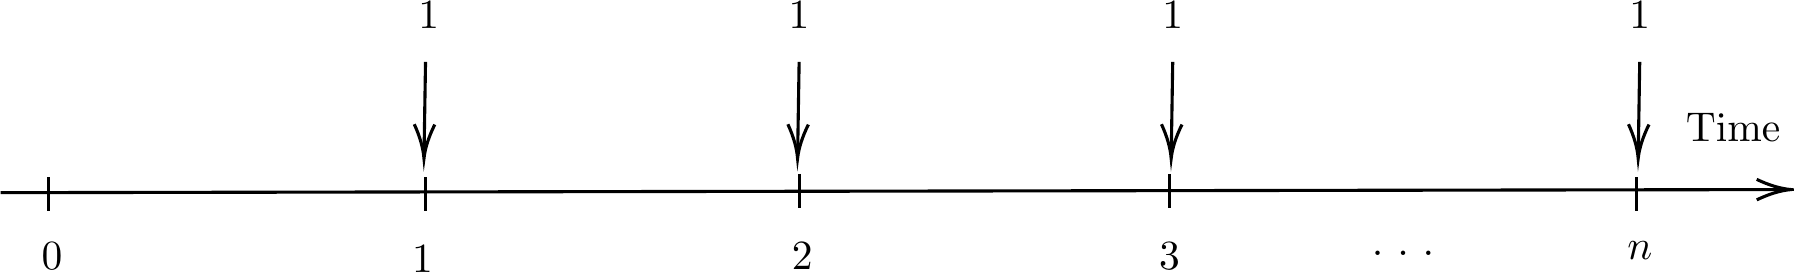
\includegraphics{SCMA266Bookdownproj_files/figure-latex/tikz-ex9-1} \end{center}

\textbf{Solution:} Based on the first principles,

\begin{align} 
 s_\angl{n} &= \sum_{r=1}^n C_r \cdot A(t_r,n) \\
    &= (1+i)^{n-1} + (1+i)^{n-2} + \ldots + (1+i) + 1. \label{eq:firstEq} 
\end{align}

Multiplying Eq.\eqref{eq:firstEq} through by (1+i) gives \begin{equation}
    (1+i) \cdot s_\angl{n}  = (1+i)^{n} + (1+i)^{n-1} + \ldots + (1+i)^2 + (1+i). 
\end{equation} Subtracting the two equations results in
\[\begin{aligned}
    i \cdot s_\angl{n} &= (1+i)^{n} - 1\\
        s_\angl{n} &= \frac{(1+i)^{n} - 1}{i}.\end{aligned}\]

\begin{example}
\emph{Let} \(i\) be the constant effective rate of interest per time unit. Show
that the present value at time 0 of a level annuity certain, denoted by
\(a_\angl{n}\) (pronounced ``A.N.'') , having cashflow of 1 unit at the end
of each of the next \(n\) time units is
\[a_\angl{n} = \frac{1 - v^n }{i}.\]
\end{example}

\textbf{Solution:} Taking the accumulated value at time \(n\) and discounting
back to time 0 gives \[\begin{aligned}
    a_\angl{n} &= s_\angl{n} \cdot v^n \\
            &= \frac{(1+i)^{n} - 1}{i} \cdot v^n \\
            &=  \frac{1 - v^n }{i}.\end{aligned}\]

\begin{example}

\emph{Given the effective rate of interest of} \(8\%\) p.a., calculate

\begin{enumerate}
\def\labelenumi{\arabic{enumi}.}
\item
  \emph{the accumulation at 12 years of ฿500 payable yearly in arrears for
  the next 12 years.}
\item
  \emph{the present value now of ฿2,000 payable yearly in arrears for the
  next 6 years.}
\item
  \emph{the present value now of ฿1,000 payable half-yearly in arrears for
  the next 12.5 years.}
\end{enumerate}

\end{example}

\textbf{Solution:}

\begin{enumerate}
\def\labelenumi{\arabic{enumi}.}
\tightlist
\item
  The timeline of this transaction is shown in the figure below.
\end{enumerate}

\begin{center}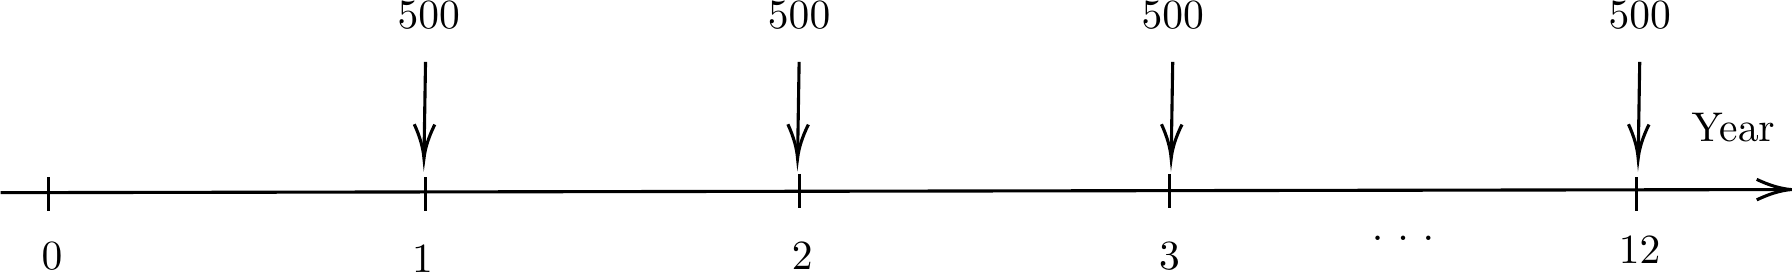
\includegraphics{SCMA266Bookdownproj_files/figure-latex/tikz-ex10-1} \end{center}

The accumulation of the payments is

\[500 \cdot s_\angl{12}  = 500 \cdot \frac{1.08^{12} - 1 }{0.08 } = 9488.563230.\]

\begin{enumerate}
\def\labelenumi{\arabic{enumi}.}
\setcounter{enumi}{1}
\item
  The present value of the payments is
  \[2000\cdot a_\angl{6}  = 2000 \cdot \frac{1 - 1.08^{-6} }{0.08 } = 9245.759328.\]
\item
  An interest rate of 8\% p.a. is equivalent to an effective
  half-yearly interest rate, denoted by \(j\), of
  \[j = 1.08^{1/2} -1 = 0.039230.\] There are 25 payments of 1000
  each, starting in six months' time.

  Working in terms of half year, the present value of the payment is
  \[1000 \cdot a^j_\angl{25} = 1000 \cdot \frac{1 - 1.039230^{-25} }{0.039230 } = 15750.003911.\]
\end{enumerate}

\subsection{Level Annuities Due}\label{level-annuities-due}

An \emph{annuity-due} is an annuity where the payments made at the start of
each time period (instead of a the end), i.e.~the payments are paid \emph{in
advance}.

In order to calculate the present value or accumulation of an annuity
due, we first introduce the concept of the rate of discount.

\subsubsection*{The rate of discount}\label{the-rate-of-discount}
\addcontentsline{toc}{subsubsection}{The rate of discount}

As opposed to the interest rate where the accumulation of initial
investment can be obtained by multiplying it by the accumulation factor
\((1+i)^n\), we can obtain the discounted value of payment by using
discount rates.

Suppose an amount of ฿1 is due after 1 year with an effective rate of
\(i \%\) p.a. (see the timeline below). What is the amount of money
required to invested now to accumulate to 1?

\begin{center}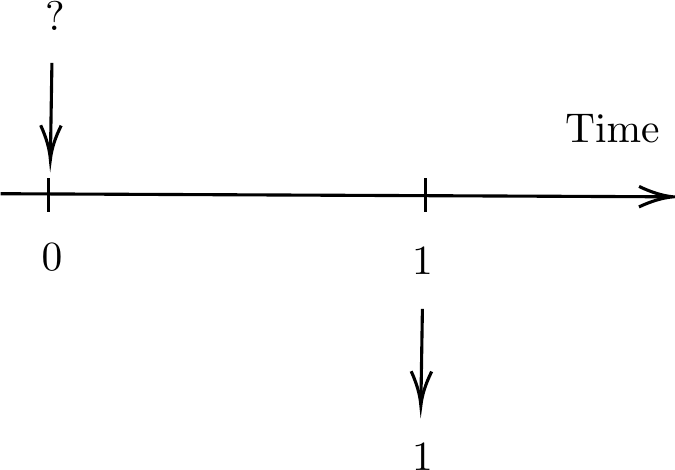
\includegraphics{SCMA266Bookdownproj_files/figure-latex/tikz-ex12-1} \end{center}

The amount of money required now to accumulate to ฿1 in one year is
\[v =  \frac{1}{1+i}.\] Note that \[\frac{1}{1+i} = 1 - \frac{i}{1+i}.\]
We define the effective rate of discount \(d\) per annum
as\[d = \frac{i}{1+i}.\] It follows that
\[v = \frac{1}{1+i} = 1 - \frac{i}{1+i} =  1 - d\] represents the
discount of ฿1 for 1 year using the effective rate of interest of \(i \%\)
p.a.

Similarly, suppose an amount of ฿1 is due after \(n\) year with an
effective rate of \(i \%\) p.a. The amount of money required to invested
now to accumulate to 1 in \(n\) year is \[\frac{1}{(1+i)^n} = (1-d)^n.\]
See the timeline below for illustration.

\begin{center}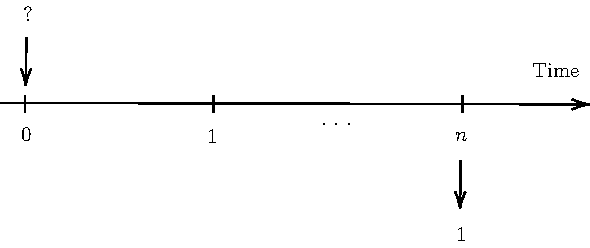
\includegraphics{SCMA266Bookdownproj_files/figure-latex/tikz-ex14-1} \end{center}

\begin{example}
\emph{Discount ฿2,000 for 3 years using the effective rate of discount of 5\%
per annum.}
\end{example}

\textbf{Solution:} After 1 year the discount will be \(0.05 \cdot 2000 = 100,\)
and the discounted value of the payment will be
\[2000 \cdot (1 - d) = 2000 \cdot (1 - 0.05) = 1900 .\] Similarly, after
2 years, the discounted value will be
\[2000 \cdot (1 - d)^2 = 2000 \cdot (1 - 0.05)^2 = 1805 .\] After 3
years, the discounted value of the payment will be
\[2000 \cdot (1 - d)^3 = 2000 \cdot (1 - 0.05)^3 = 1714.75 .\]

\begin{example}
\emph{The effective rate of discount} \(d\) per time unit can be regarded as
the interest paid in advance at time 0, which is equivalent to the
effective rate of interest \(i\) payable in arrears.
\end{example}

\textbf{Solution:} To show this, suppose that the bank added interest of \(x\)
to an account of an amount of 1 unit at the start of the period. Assume
that the interest amount of \(x\) can be withdrawn and invested in another
bank that earn the rate of interest \(i\%\) effective per time unit. The
principle of 1 unit is still in the first bank.

\begin{center}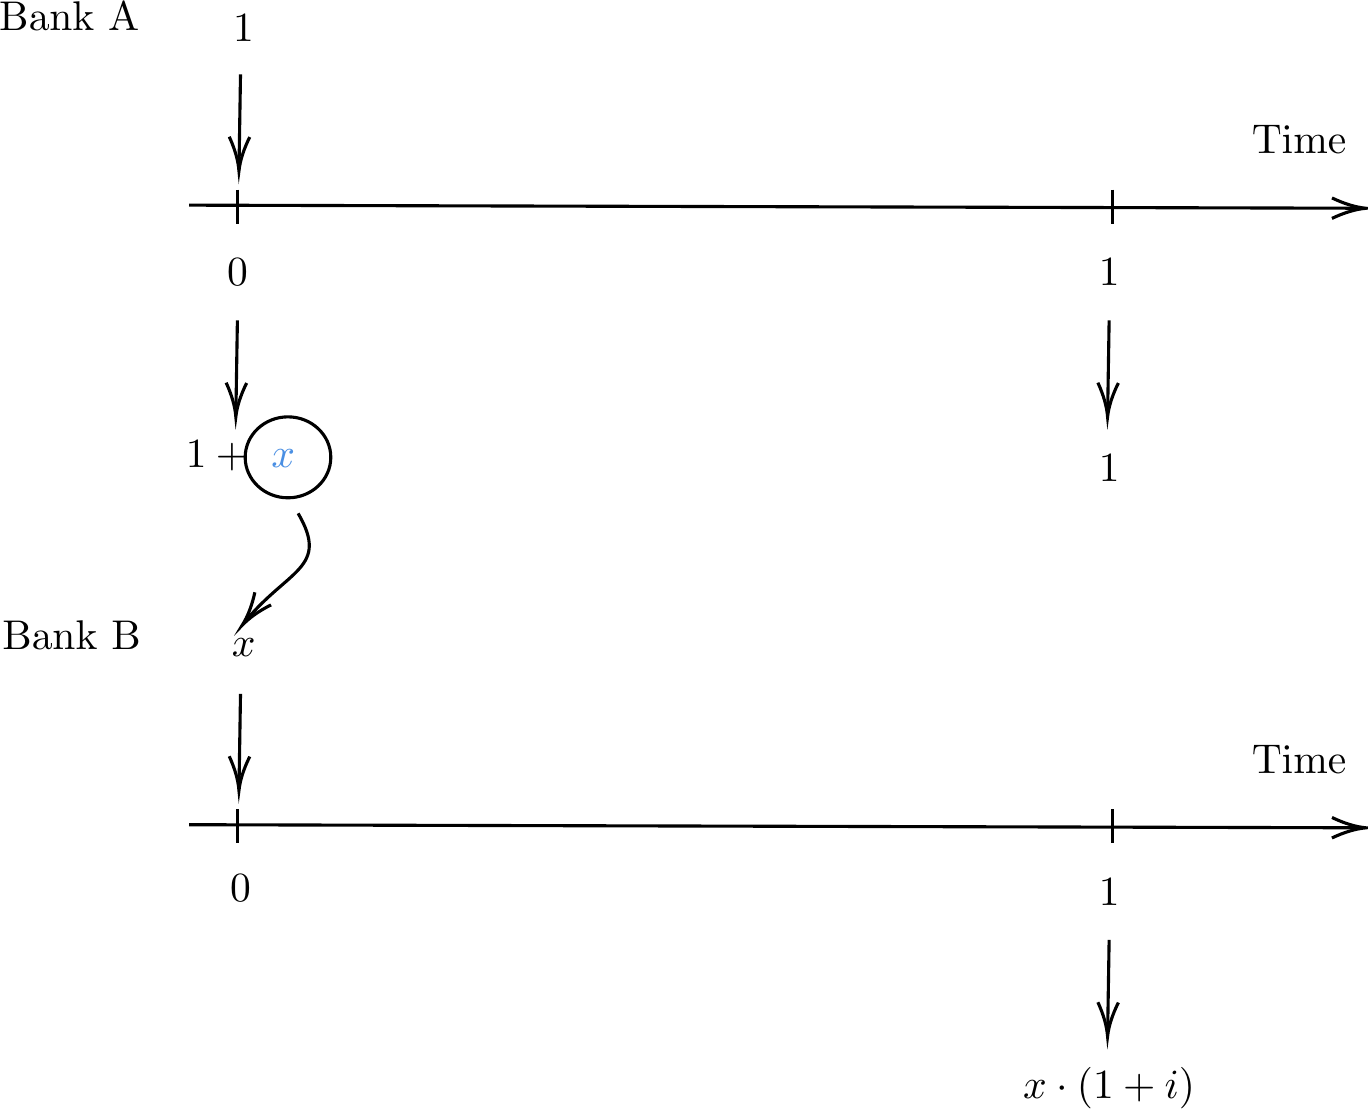
\includegraphics{SCMA266Bookdownproj_files/figure-latex/tikz-ex15-1} \end{center}

At the end of the year, we have

\begin{itemize}
\item
  the principle of 1 unit in the first bank, and
\item
  the interest paid in advance which accumulates to \(x(1+i)\) in the
  second bank.
\end{itemize}

For this to be equivalent to the interest paid in arrears, we can find
\(x\) which solves \[\begin{aligned}
     1 + x(1+i) &= 1 + i,\\
     x &= \frac{i}{1+i} = \frac{1+i}{1+i} - \frac{1}{1+i}  = 1-v = d.\end{aligned}\]
Therefore, the effective rate of discount \(d\) per time unit can be
regarded as the interest paid in advance at time 0, which is equivalent
to the effective rate of interest \(i\) payable in arrears.

\begin{example}
\emph{Let} \(i\) be the constant effective rate of interest per time unit. Show
that the accumulated value of a level annuity due, denoted by
\(\ddot{s}_\angl{n}\) (pronounced ``S-due N'', having cashflow of 1 unit at
the start of each of the next \(n\) time units is
\[\ddot{s}_\angl{n} = \frac{(1+i)^n -1 }{d}.\]
\end{example}

\begin{center}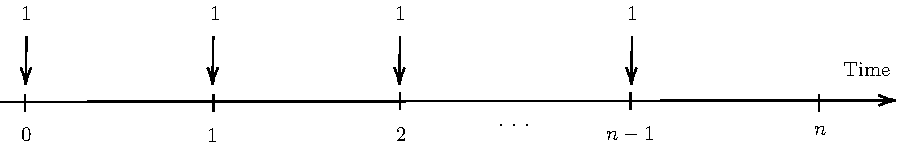
\includegraphics{SCMA266Bookdownproj_files/figure-latex/tikz-ex16-1} \end{center}

\textbf{Solution:} Using the previous results, it follows that
\[\begin{aligned}
 \ddot{s}_\angl{n} &= (1+i)^n + (1+i)^{n-1} + \cdots + (1+i)^2 + (1+i) \\
            &= (1+i) \cdot \left[(1+i)^{n-1} + \cdots + (1+i)^1 + 1\right] \\
            &= (1+i) \cdot {s}_\angl{n} \\
            &= (1+i) \cdot \frac{(1+i)^n -1 }{i}\\
            &=  \frac{(1+i)^n -1 }{i/(1+i)}\\
            &=  \frac{(1+i)^n -1 }{d}.\end{aligned}\]

\begin{example}
\emph{Let} \(i\) be the constant effective rate of interest per time unit. Show
that the present value at time 0 of a level annuity due having cashflow
of 1 unit at the start of each of the next \(n\) time units is
\[\ddot{a}_\angl{n} =  \frac{1 - v^n }{d}.\]
\end{example}

\textbf{Solution:} The present values of the payments can be obtained by
discounting \(\ddot{a}_\angl{n}\) back to time 0, i.e.~\[\begin{aligned}
 \ddot{a}_\angl{n} &= v^n  \cdot  \ddot{s}_\angl{n} \\
            &= v^n  \frac{(1+i)^n -1 }{d} \\
            &=\frac{1 - v^n}{d}.\end{aligned}\]

\begin{example}

\emph{Given the effective rate of interest of} \(8\%\) p.a., calculate

\begin{enumerate}
\def\labelenumi{\arabic{enumi}.}
\item
  \emph{the accumulation at 12 years of ฿500 payable yearly in advance for
  the next 12 years.}
\item
  \emph{the present value now of ฿2,000 payable yearly in advance for the
  next 6 years.}
\item
  \emph{the present value now of ฿1,000 payable half-yearly in advance for
  the next 12.5 years.}
\end{enumerate}

\end{example}

\textbf{Solution:}

\begin{enumerate}
\def\labelenumi{\arabic{enumi}.}
\item
  The accumulation of the annuity-due of 12 years is
  \[500 \cdot \ddot{s}_\angl{12} = 500 \cdot \frac{1.08^{12} -1}{0.08/1.08} = 10247.648289.\]
\item
  The present value of the annuity-due of 6 years is
  \[2000 \cdot \ddot{a}_\angl{6} = 2000 \cdot \frac{1- 1.08^{-6}}{0.08/1.08} = 9985.420074.\]
\item
  An interest rate of 8\% p.a. is equivalent to an effective
  half-yearly interest rate, denoted by \(j\), of
  \[j = 1.08^{1/2} -1 = 0.039230.\] There are 25 payments of 1000
  each, starting in six months' time.

  Working in terms of half year, the present value of the payment is
  \[1000 \cdot \ddot{a}^j_\angl{25} = 1000 \cdot \frac{1 - 1.039230^{-25} }{0.039230/1.039230 } = 16367.876564.\]
\end{enumerate}

\subsection{Deferred annuities}\label{deferred-annuities}

An annuity whose first payment is made during the first time period
(either in arrears or in advance) is called \emph{immediate annuity}.
Otherwise, the annuity is known as \emph{deferred} annuity, i.e.~the first
payment starts some time in the future.

To calculate the present value of the annuity of a series of \(n\)
payments deferred for \(m\) time units (the first payment is due at time
\(m+1\)), denoted by \(_{m \textbar}a_\angl{n}\), we first calculate the
present value at the end of the deferred period and then discount back
to the start of the period.

\begin{center}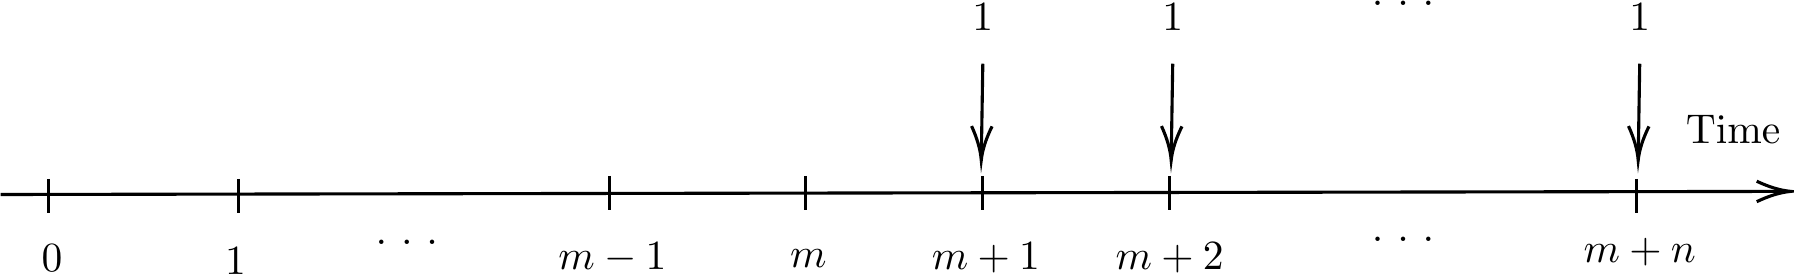
\includegraphics{SCMA266Bookdownproj_files/figure-latex/tikz-ex17-1} \end{center}

\[\begin{aligned}
    _{m \textbar} a_\angl{n}  &= v^{m+1} + v^{m+2} + \cdots +v^{m+n}  \\
    &= v^m  \left( v + v^2 + \cdots + v^n  \right) \\
    &= v^m \cdot  a_\angl{n}.\end{aligned}\]

\begin{example}
\emph{Calculate the present value at time 0 of an annuity of 1 p.a. in
arrears for 6 years and deferred for 10 at 6\% effective rate p.a.}
\end{example}

\begin{center}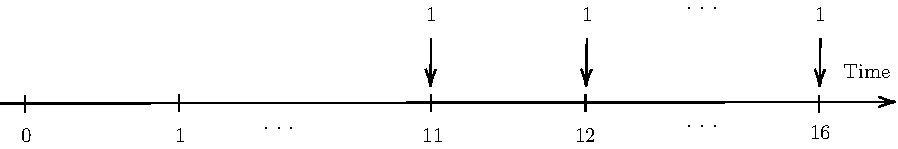
\includegraphics{SCMA266Bookdownproj_files/figure-latex/tikz-ex18-1} \end{center}

This is an annuity with 6 unit payments for which the first payment is
at time 11. Hence the present values of such payments is
\[\begin{aligned}
    _{10 \textbar}a_\angl{6}
  &= v^{11} + v^{12} + \cdots +v^{16}  \\
    &= v^{10}  \left( v + v^2 + \cdots + v^6  \right) \\
    &= v^{10} \cdot  a_\angl{6} \\
    &= \left(\frac{1}{1.06}\right)^{10} \cdot \left( \frac{1- 1.06^{-6}}{0.06} \right)
    &= 2.745808.\end{aligned}\]

\begin{example}

\emph{Give the reason or show that the present value of a series of} \((n+m)\)
payments of one unit payable at the end of each time period is equal to
the sum of

\begin{enumerate}
\def\labelenumi{\arabic{enumi}.}
\item
  \emph{present value of} \(m\) payments of one units payable at the end of
  each time period (denoted by \(a_\angl{m}\)) and
\item
  \emph{present value of} \(n\) payments of one units payable at the end of
  each time period deferred for \(m\) years (denoted by
  \(_{m \textbar}a_\angl{n}\)).
\end{enumerate}

\end{example}

\textbf{Solution:} The present value of a series of (m+n) payments is
\[\begin{aligned}
a_\angl{m+n} &=  \left( v + v^2 + \cdots  v^m\right) + \left( v^{m+1} + v^{m+2} + \cdots +v^{m+n} \right) \\
&= a_\angl{m} + _{m \textbar}a_\angl{n}.\end{aligned}\] It follows that
\(_{m \textbar}a_\angl{n} = a_\angl{m+n} - a_\angl{m}.\)

\subsection{Increasing annuities}\label{increasing-annuities}

An annuity in which the \(i\)th payment of the amount \(i\) is made at time
\(t_i = i\) is called an \emph{(simple) increasing} annuity. The present and
accumulated value of this annuity can be obtained from the first
principles. For example, the present value of the increasing annuity can
be evaluated by \[\sum_{i=1}^n X_i v^{t_i} = \sum_{i=1}^n i v^{t_i},\]
where the \(i\)th payment of amount \(X_i = i\) at time \(t_i = i\).

\begin{example}
\emph{Derive the formula for the present value of a simple increasing annuity
payable yearly in arrears with the effective rate} \(i\%\) p.a. for \(n\)
years.
\end{example}

\textbf{Solution:} The cashflows of the simple increasing annuity payable
yearly in arrears is illustrated below. The present value of payments of
1 at time 1, 2 at time 2, \(\ldots, n\) at time \(n\) denoted by
\((Ia)_\angl{n}\) is given by
\[(Ia)^{i}_\angl{n}   = \frac{\ddot{a}^{i}_{\actuarialangle{n}} - nv^n}{i}.\]

\begin{center}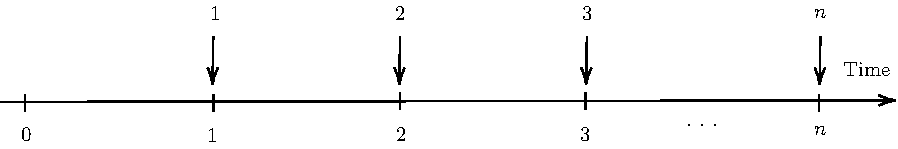
\includegraphics{SCMA266Bookdownproj_files/figure-latex/tikz-ex19-1} \end{center}

\textbf{Notes}

\begin{enumerate}
\def\labelenumi{\arabic{enumi}.}
\item
  An increasing annuity but with payments in advance is given by
  \[(I\ddot{a})^{i}_\angl{n}   = \frac{\ddot{a}^{i}_{\actuarialangle{n}} - nv^n}{d}.\]
\item
  The formulas for the accumulated values are
  \[(Is)^{i}_\angl{n} = \frac{\ddot{s}^{i}_{\actuarialangle{n}} - n}{i} \quad\text{(in arrears)}\]
  \[(I\ddot{s})^{i}_\angl{n} = \frac{\ddot{s}^{i}_{\actuarialangle{n}} - n}{d} \quad\text{(in advance)}\]
\end{enumerate}

\subsection{Compound increasing annuities}\label{compound-increasing-annuities}

The following example considers the value of compound increasing
annuities where the payments increase by a constant factor each time.

\begin{example}
\emph{Assume that the effective rate of interest is 6\% p.a. Calculate the
present value as at 1 January 2010 of an annuity payable annually in
arrears for 8 years. The first payment is ฿10 and subsequent payments
increase by 2\% per annum compound.}
\end{example}

\textbf{Solution:}

\begin{center}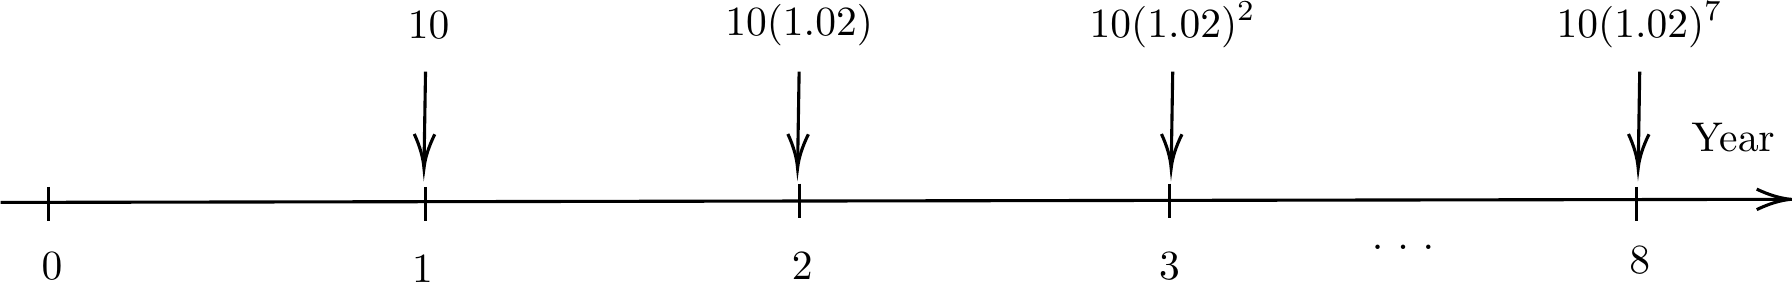
\includegraphics{SCMA266Bookdownproj_files/figure-latex/tikz-ex20-1} \end{center}

At 1/1/2010, the present value of the payment is given by
\[\begin{aligned}
    PV &= 10 \cdot \frac{1}{1.06} + 10 \cdot \frac{1.02}{(1.06)^2} + \cdots +  10 \cdot \frac{(1.02)^7}{(1.06)^8} \\
        &= \frac{10}{1.02} \left(  \frac{1.02}{1.06} +  \left(  \frac{1.02}{1.06}  \right)^2 + \cdots +
    \left(  \frac{1.02}{1.06}  \right)^8  \right)\end{aligned}\] The
above equation can be arranged so that the annuity formula can be
applied. We can define \(j\) such that \(1 + j = 1.06/1.02\), and hence,
\[\begin{aligned}
    PV &= \frac{10}{1.02} \left(  \frac{1}{1 + j} +  \left(  \frac{1}{1+j}  \right)^2 + \cdots +
    \left(  \frac{1}{1+j}  \right)^8  \right)  \\
    &=   \frac{10}{1.02}  a_\angl{8} \quad  \text{ at } j\% \\
    &=  \frac{10}{1.02} \left(   \frac{1 - \left(\frac{1.02}{1.06}\right)^8   }{\left(   \frac{1.06}{1.02}   - 1 \right)}  \right) \\
    &= 66.2216\end{aligned}\]

\subsection{Annuities payable more than once per time unit}\label{annuities-payable-more-than-once-per-time-unit}

Consider the value of an annuity payable in arrears \(m\) times per time
unit at an effective rate of interest \(i\) per time unit. The annuity is
still payable for \(n\) time units and a total amount of 1 unit per time
unit. The present and accumulated values of the corresponding annuity
are denoted by \(a^{(m)i}_\angl{n}\) and \(s^{(m)i}_\angl{n}\),
respectively.

To calculate either the present or accumulation value of this annuity,
we can simply apply the first principles by using the effective rate of
interest per \(1/m\) time unit. In particular, we have
\[a^{(m)i}_\angl{n}   = \frac{1}{m}  a^j_\angl{n\cdot m},\] and
\[s^{(m)i}_\angl{n}   = \frac{1}{m}  s^j_\angl{n\cdot m},\] where \(j\) is
the effective rate per \(1/m\) time unit.

\begin{example}
\emph{Calculate the accumulation at 1 January 2020 of an annuity of ฿100 per
month, payable in arrears from 1 January 2010 at an effective rate of
interest of 4\% p.a.}
\end{example}

\textbf{Solution:} The annual payment is 1200 and the effective rate per
month equivalent to 4\% p.a. is \(j = (1.04)^{1/12} - 1 = 0.003274\) per
month. Hence,
\[1200 s^{(12)4\%}_\angl{10}   = 100  s^j_\angl{12\cdot 10} = 14669.59.\]

\section{Nominal Rates of Interest}\label{nominal-rates-of-interest}

Nominal interest rates are the interest rates before taking inflation
into account. They may also refer to the advertised (in bank accounts)
or stated rates of interest on a loan, without regard to fees or
compound interest. Throughout this section, the time unit used is
assumed to be \textbf{one year}.

\begin{itemize}
\item
  \textbf{Effective rate of interest} is the interest \(i\) paid at the end
  of the year on an amount ฿1 at the start of the year.
\item
  \textbf{Nominal interest rate payable} \(p\) times per period, denoted by
  \(i^{(p)}\) is an effective rate of interest of \(i^{(p)}/p\) applied
  for each \(p\)th of a period. The interest is paid more frequently
  than once per measurement period.
\end{itemize}

The nominal rate of interest payable \(p\) times per period is also known
as \textbf{the rate of interest convertible} \(p\)thly or compounded \(p\)thly.

\begin{example}
\emph{A nominal rate of interest of} \(i^{(4)} = 10\%\) p.a. convertible
quarterly means an interest rate of 10/4 = 2.5\% per quarter effective.
Calculate the accumulated value in 1 year of a payment of ฿100 at the
given nominal rate.
\end{example}

\textbf{Solution:} When working with the nominal interest rate, the nominal
interest rate is often converted to an effective interest rate. In this
example, the nominal interest rate \(i^{(4)} = 10\%\) is equivalent to an
effective interest rate of \(2.5\%\) per quarter. The accumulated value in
1 year is \(100 (1 + 2.5\%)^4 = 110.3813\). After compound interest is
taken into account, the interest income of an investor at the quarterly
convertible nominal interest rate of 10\% p.a. is 10.3813 (or 10.3813\%.
p.a. effective)

\textbf{Nominal} is used where interest is paid more frequently than once per
unit year.

\begin{example}
\emph{At a rate of 12\% p.a. effective, draw a timeline to show cashflows if
฿100 is invested at the start of the year.}
\end{example}

\textbf{Solution:} The accumulated value of ฿100 at the end of the year is
\(100 (1 + 12\%) = 112\).

\begin{example}
\emph{At a rate of 12\% p.a. compounding quarterly, draw a time line to show
cashflows if ฿100 is invested at the start of the year.}
\end{example}

\textbf{Solution:} The nominal interest rate \(i^{(4)} = 12\%\) is equivalent
to an effective interest rate of \(3\%\) per quarter. The accumulated
value in 1 year is \(100 (1 + 3\%)^4 = 112.55\). After compound interest
is taken into account, the interest income of an investor at the
quarterly convertible nominal interest rate of 10\% p.a. is 12.55 (or
12.55\%. p.a. effective)

\(i^{(p)}\) is an effective rate of interest of \(i^{(p)}/p\) applied for
each \(p\)th of a period. The interest is paid more \(p\) times per
measurement period (i.e.~per year). The value at time can be regarded as
the annuity having cashflow of \(i^{(p)}/p\) per each period as shown in
the figure below. Therefore, the accumulated value in 1 year can also be
calculated as \(100( 1 + 0.03 s_{\angl{4}}^{3\%})\).

\textbf{Note} In practice, it is easier to work with the effective rate of
interest which is defined in a suitable time unit.

The following formula can be used to convert between the effective rate
\(i\) p.a. and the nominal rate \(i^{(m)}\) p.a.:
\[( 1 + i) = \left( 1 + \frac{i^{(m)}}{m}\right)^m.\]

\begin{example}
\leavevmode

\begin{enumerate}
\def\labelenumi{\arabic{enumi}.}
\item
  \emph{Express a nominal annual interest rate of 9\% convertible
  half-yearly as a monthly effective interest.}
\item
  \emph{Express a two-monthly effective interest of 3\% as a nominal annual
  interest rate convertible two-monthly.}
\end{enumerate}

\end{example}

\textbf{Solution:}

\begin{enumerate}
\def\labelenumi{\arabic{enumi}.}
\item
  The effective rate \(i\)\% p.a. is \[i = ( 1 + \frac{0.09}{2})^2 - 1.\]
  Hence the monthly effective rate is
  \(j = (1 + i)^{1/12} - 1 = ( 1 + \frac{0.09}{2})^{2/12} - 1 = 0.007363\).
\item
  A nominal annual interest rate convertible two-monthly is
  \(6 \cdot 3\% = 18\%\).
\end{enumerate}

\begin{example}

\emph{Express each of the following effective rates per annum as a nominal
rate, and vice versa.}

\begin{longtable}[]{@{}ll@{}}
\toprule\noalign{}
\textbf{\emph{Effective Rate}} & \textbf{\emph{Nominal Rate}} \\
\midrule\noalign{}
\endhead
\bottomrule\noalign{}
\endlastfoot
\(i\) = 0.04 & \(i^{(4)} = 0.039412\) \\
\(i\) = 0.10 & \(i^{(12)} = 0.095690\) \\
\(i\) = 0.06152 & \(i^{(2)} = 0.06\) \\
\(i\) = 0.126825 & \(i^{(12)} = 0.12\) \\
\end{longtable}

\end{example}

\subsection{Nominal Rates of Discount}\label{nominal-rates-of-discount}

The effective rate of discount per annum is \(d = 1 -v\). It is the amount
of interest payable at the start of the time unit which is equivalent to
\(i\) payable at the end of the time unit.

\textbf{The nominal rate of discount payable} \(p\) times per period \(d^{(m)}\)
(or convertible \(p\)thly or compounded \(p\)thly is interest of \(d^{(m)}/m\)
paid at the start of each \(1/m\) of a year.

The relationship between the effective discount rate \(d\) p.a. and the
nominal rate of discount payable \(m\) times a year is
\[1 - d = \left(1 - \frac{d^{(m)}}{m}\right)^m.\]

\begin{example}
\leavevmode

\begin{enumerate}
\def\labelenumi{\arabic{enumi}.}
\item
  \emph{Express a nominal annual discount rate of 6\% convertible
  half-yearly as an annual effective discount.}
\item
  \emph{Express an effective discount of 10\% per half year as a nominal
  annual discount rate convertible quarterly.}
\end{enumerate}

\end{example}

\textbf{Solution:}

\begin{enumerate}
\def\labelenumi{\arabic{enumi}.}
\item
  The annual effective discount \(d\) is
  \[d = 1-  \left(1 - \frac{d^{(m)}}{m}\right)^m = 1-  \left(1 - \frac{6\%}{2}\right)^2 = 0.0591 = 5.91\% \text{ per annum}.\]
\item
  We know that the discount factor \(v\) and the rate of discount \(d\)
  satisfy the following equation. \[v =  1- d.\] Hence the discount
  factor over half-year is \(1 - 0.1 = 0.9\). The discount factor \(v\)
  for one year (or 2 half-year) is \[(1-0.1)^2 = 0.9^2 = 0.81.\] It
  follows that the discount rate per annum is \(d = 1- 0.81 = 0.19\),
  and the nominal annual discount rate convertible quarterly \(d^{(4)}\)
  is given by \[\begin{aligned}
       d^{(m)} &= m \cdot \left( 1-      (1 - d)^{1/m}  \right) \\
       d^{(4)} &= 4 \cdot \left( 1-      (1 - 0.19)^{1/4}  \right) = 0.205267.
      \end{aligned}\]
\end{enumerate}

\section{Principle of Equivalence, Yields and Equation of Value}\label{principle-of-equivalence-yields-and-equation-of-value}

The principle of equivalence is used to compare two different cashflows
whether one is worth more than the other.

Consider two sequences of cashflows

\begin{itemize}
\item
  \(C_1, C_2, \ldots\) with payments at times \(t_1, t_2, \ldots\) and
\item
  \(D_1, D_2, \ldots\) with payments at times \(s_1, s_2, \ldots\).
\end{itemize}

Assume that the interest rates are given and apply to both of them. The
two sequences of cashflows are said to be \textbf{equivalent} (or equal in
value) if their values at any time \(t\) are the same, i.e.~there exists
\(t \in \mathbb{R}\) such that \[PV^C(t)  = PV^D(t).\]

\textbf{Notes}

\begin{enumerate}
\def\labelenumi{\arabic{enumi}.}
\item
  If two sequences of cashflows have the same value at time \(s\), then
  they have the same value at any time \(t\) since

  \begin{itemize}
  \item
    for \(t \le s\),

    \(\text{(Value at time t)} = \text{(Value at time s)} \times V(t,s),\)
  \item
    for \(t \ge s\)

    \(\text{(Value at time t)} = \text{(Value at time s)} \times A(s,t).\)
  \end{itemize}
\item
  The two sequences of cashflows are \textbf{indifferent} if their present
  values are the same.
\item
  The principle of equivalent can be applied for \textbf{pricing a financial
  security}, for example, a price \(P\) which will be paid by the
  investor in return for a series of future cashflows.
\end{enumerate}

\begin{example}
\emph{Calculate the maximum price an investor wish to pay in return for an
investment that will pay ฿500 at the end of each of the next 15 months
given that the interest rate is 0.2\% per month.}
\end{example}

The present value of these payments of 500 at the end of the next 15
months is
\[PV(0) = 500 a^{0.002}_{\angl{15}} =  500 \cdot \left(  \frac{1 - (1.002)^{-15}}{0.002}  \right)   = 7381.35.\]
Therefore, the investor would be willing to pay a maximum of 7381.35.

\begin{example}

\emph{Determine whether the following series of cashflows are equivalent
given that an interest rate is 6\% per annum effective.}

\begin{enumerate}
\def\labelenumi{\arabic{enumi}.}
\item
  \emph{One single payment of amount 6,691.127888 at year 5.}
\item
  \emph{a level annuity of 300 payable yearly in arrears for the next 5
  years plus a lump sum of 5,000.}
\item
  \emph{a level annuity of 1,186.982002 payable yearly in arrears for the
  next 5 years.}
\end{enumerate}

\end{example}

\textbf{Solution:}

\begin{enumerate}
\def\labelenumi{\arabic{enumi}.}
\item
  The present value is \(6,691.127888 \times (1.06)^{-5} = 5000\).
\item
  The present value is
  \[300 a^{0.06}_{\angl{5}}   + 5000 \times (1.06)^{-5}  = 5000.\]
\item
  The present value is \[1186.982002 a^{0.06}_{\angl{5}}     = 5000.\]
\end{enumerate}

Therefore, the three series of cashflows are \textbf{indifferent}.

\subsection{Equation of value and yields}\label{equation-of-value-and-yields}

Consider a transaction from an investment that offers

\begin{itemize}
\item
  to pay an investor of amounts (i.e.~money received)
  \(B_1, B_2, \ldots, B_n\) at time \(t_1, t_2, \ldots ,t_n\)
\item
  in return for outlays (i.e.~money paid out) of amounts
  \(A_1, A_2, \ldots, A_n\) at these times, respectively.
\end{itemize}

Only one of \(A_i\) and \(B_i\) will be non-zero in general.

\textbf{An equation of value} equates the present value of money received to
the present value of money paid out, which can be written as
\[\sum_{i=1}^n A_i v^i = \sum_{i=1}^n B_i v^i.\] The equation of value
can also be written in terms of the \textbf{net cashflow} at time \(t_i\), i.e.
\(C_t = B_t - A_t\), \[PV_i(0) = \sum_{i=1}^n C_i v^i =0.\]

Equations of value are used throughout actuarial work. Some examples are
as follows:

\begin{itemize}
\item
  The \textbf{fair price} to pay for an investment such as a fixed interest
  security or an equity (ie, \(PV\) outgo) equals the present value of
  the proceeds from the investment, discounted at the rate of interest
  required by the investor.
\item
  The \textbf{premium} for an insurance policy is calculated by equating
  the present value of the expected amounts received in premiums to
  the present value of the expected benefits and other outgo.
\end{itemize}

We shall be concerned mainly with the question:

At what rate of interest does the series of amounts paid out have the
same value as the series of amounts received? The corresponding rate of
interest is called the \textbf{yield of the cashflows} (or \textbf{internal rate of
return, money-weighted rate of return}).

\textbf{Notes}

\begin{enumerate}
\def\labelenumi{\arabic{enumi}.}
\item
  Equations of values may have no roots, a unique root or multiple
  roots.
\item
  In most practice situations, there is a unique positive real root.
\end{enumerate}

\begin{example}
\emph{An investor pays ฿1,000 in order to receive ฿600 back in 2 years and
฿800 back in 4 years. Calculate the annual effective rate of interest
earned on this investment (or the yield on the investment).}
\end{example}

\textbf{Solution:} The yield of the investment \(i\%\) satisfies the equation
of value \[PV_i(0) =  -1000 + 600(1+i)^{-2} + 800(1+i)^{-4} = 0.\] To
solve the equation for \(i\), we define \(z = (1+i)^{-2}\), resulting in
\[8z^2 + 6z - 10 = 0.\] Therefore \(z = 0.804248\) and \(i = 0.115078.\)

\begin{example}
\protect\hypertarget{exm:exampleYield}{}\label{exm:exampleYield}\emph{An investor pays ฿1,000 in order to receive ฿300 back at the end of the
first 2 years and ฿400 back at the end of the third, forth and fifth
year. Calculate the annual effective rate of interest earned on this
investment (or the yield on the investment).}
\end{example}

\textbf{Solution:} The yield of the investment \(i\%\) p.a. satisfies the
equation of value
\[PV_i(0) =  -1000 + \frac{300}{(1+i)} + \frac{300}{(1+i)^{2}} + \frac{400}{(1+i)^{3}} +  \frac{400}{(1+i)^{4}} + \frac{400}{(1+i)^{5}}.\]
In our next section, we will learn how to approximate the yield of the
above equation.

\subsection{The method to estimate the yield}\label{the-method-to-estimate-the-yield}

By using linear interpolation, the yield can be estimated as follows.
Let \(P_1\) and \(P_2\) be the present values calculated at interest rates
\(i_1\) and \(i_2\), respectively. Then the interest rate corresponding to a
present value of \(P\) can be approximated by
\[i \approx i_1 + (i_2 - i_1) \frac{P - P_1}{P_2 - P_1}.\] In order to
apply this method to calculate the yield \(i\), we simply set \(P = 0\), and
hence \[i \approx i_1 + (i_2 - i_1) \frac{ - P_1}{P_2 - P_1}.\]

\begin{figure}
\centering
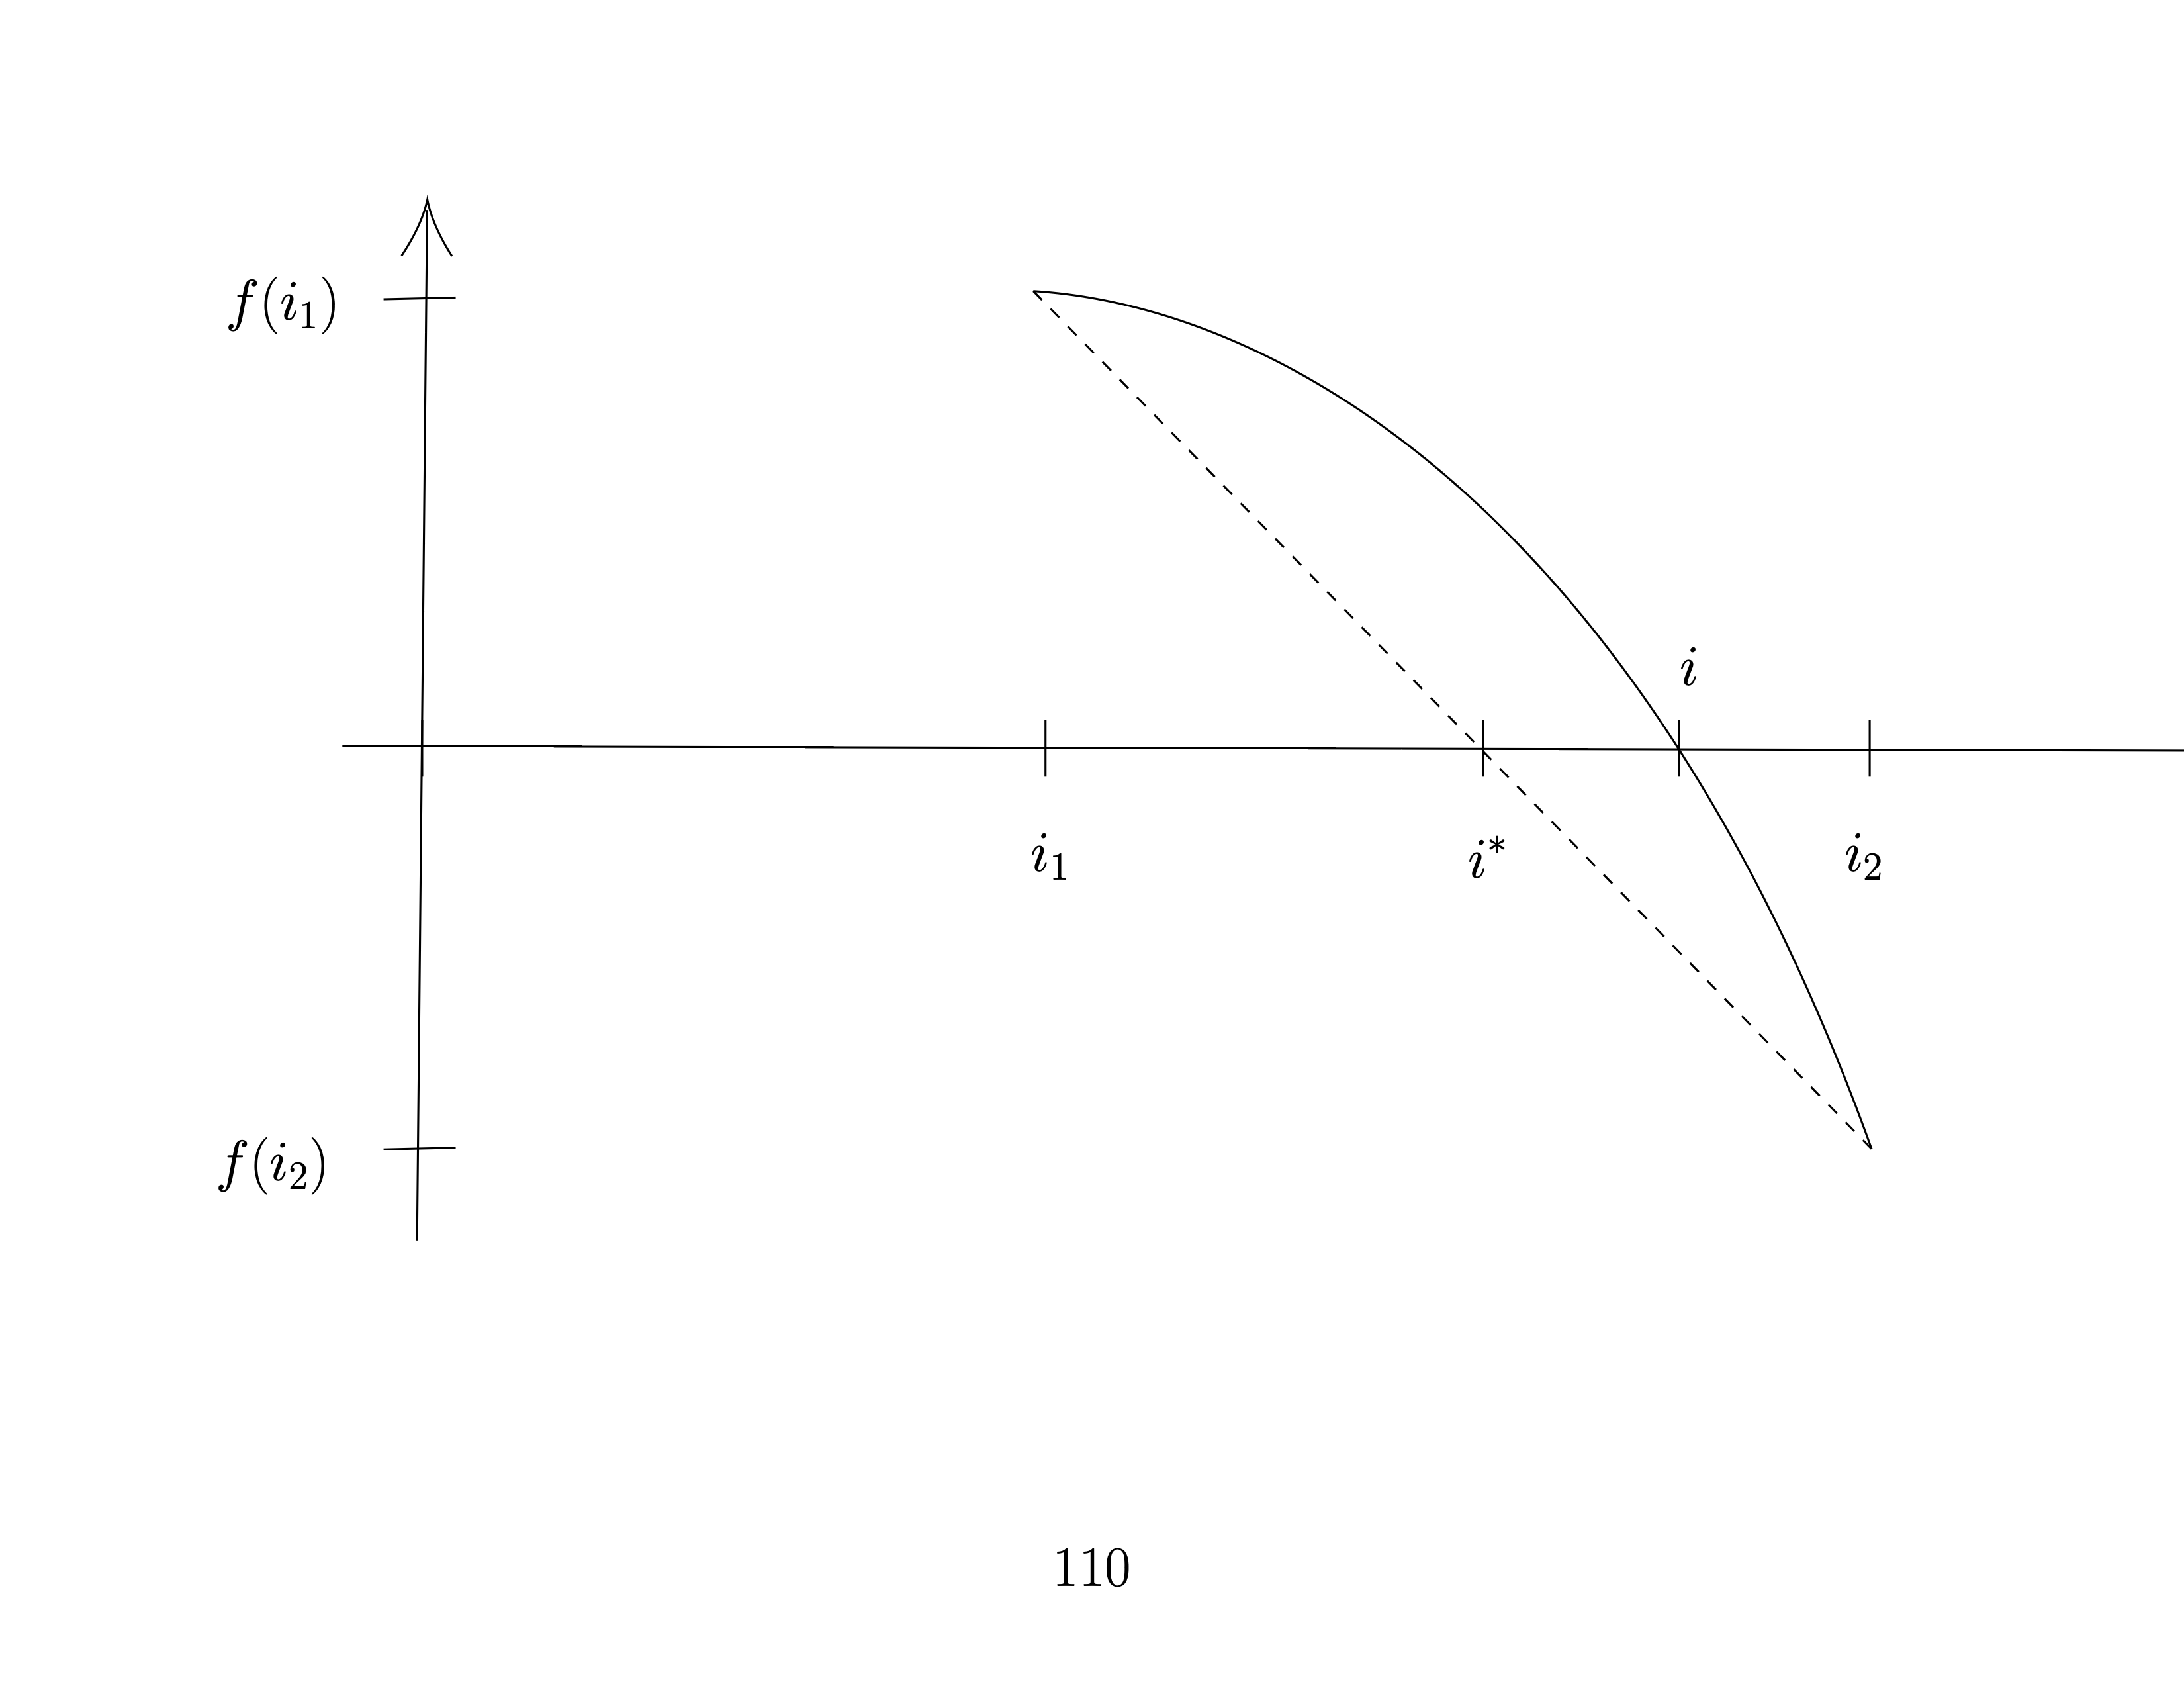
\includegraphics{Yield_figure.png}
\caption{Components of Financial markets}
\end{figure}

From the figure above, the yield \(i\) can be approximated by \(i^*\), which
is the \(x\)-intercept of the straight line joining the points \((i_1,P_1)\)
and \((i_2,P_2)\). From
\[\frac{i^* -i_1}{i_2 - i_1} = \frac{P_{i^*} - P_1}{P_2 - P_1},\] we
have \(P_{i^*} = 0\) and
\[i \approx i^* =  i_1 + (i_2 - i_1) \frac{ - P_1}{P_2 - P_1}.\] Note
that one can get a good approximation by taking values that are either
side of the true value and about 1\% apart.

\begin{example}
\emph{Approximate the yield of the transaction in Example}
\ref{exm:exampleYield}\emph{.}
\end{example}

\textbf{Solution:} Here, When \(i_1 = 0.21\), \(P_1 = PV_{0.21}(0) = 19.448\) and
when \(i_1 = 0.22\), \(P_2 = PV_{0.22}(0) = -3.698.\) The yield is
approximately equal to \[\begin{aligned}
 i &\approx 0.21 - (0.22 - 0.21) \left(  \frac{19.448}{-3.698 - 19.448} \right) \\
   &= 0.218402 \text{ p.a. effective.}\end{aligned}\]

\section{Loan schedules}\label{loan-schedules}

In this section, we describe how a loan may be repaid. A schedule of
repayment together with the interest and capital components of an
annuity payment will be discussed.

Suppose that a lender lends an individual of amount \(L\) for \(n\) years
with an effective rate of interest \(i\) per annum. We say that the
\textbf{term} of the loan is \(n\) years with the loan \textbf{amount} of \(L\). How
could we repay the loan?

\subsection*{Repay as late as possible:}\label{repay-as-late-as-possible}
\addcontentsline{toc}{subsection}{Repay as late as possible:}

After \(n\) year, the borrower repays the entire loan and all interest
that accrued over the period. The total amount to be repaid is equal to

\subsection*{Repay interest only during the term and repay the capital at the end of the term:}\label{repay-interest-only-during-the-term-and-repay-the-capital-at-the-end-of-the-term}
\addcontentsline{toc}{subsection}{Repay interest only during the term and repay the capital at the end of the term:}

These types of loan where the borrower is a government or a company are
\textbf{bonds} or \textbf{fixed interest securities}.

\subsection*{Repay loan by regular instalments of interest and capital throughout term of loan:}\label{repay-loan-by-regular-instalments-of-interest-and-capital-throughout-term-of-loan}
\addcontentsline{toc}{subsection}{Repay loan by regular instalments of interest and capital throughout term of loan:}

Each repayment must pay first for interest due and the remainder is used
to repay some of the capital outstanding.

\begin{example}
\emph{You borrow ฿5,000 for a term of 3 years at a fixed interest rate of 10\%
pa. The loan is to be repaid by 3 level annual repayments of ฿2,010.57
at the end of each year. Calculate the interest content, capital content
from each repayment and capital outstanding after such repayment.}
\end{example}

\textbf{Note} The loan payments can be expressed in the form of a \textbf{Loan
Schedule} as follows:

\begin{longtable}[]{@{}
  >{\centering\arraybackslash}p{(\columnwidth - 8\tabcolsep) * \real{0.0845}}
  >{\centering\arraybackslash}p{(\columnwidth - 8\tabcolsep) * \real{0.1549}}
  >{\centering\arraybackslash}p{(\columnwidth - 8\tabcolsep) * \real{0.2254}}
  >{\centering\arraybackslash}p{(\columnwidth - 8\tabcolsep) * \real{0.2394}}
  >{\centering\arraybackslash}p{(\columnwidth - 8\tabcolsep) * \real{0.2958}}@{}}
\toprule\noalign{}
\begin{minipage}[b]{\linewidth}\centering
Time
\end{minipage} & \begin{minipage}[b]{\linewidth}\centering
Repayment
\end{minipage} & \begin{minipage}[b]{\linewidth}\centering
Intest content
\end{minipage} & \begin{minipage}[b]{\linewidth}\centering
Capital content
\end{minipage} & \begin{minipage}[b]{\linewidth}\centering
Capital outstanding
\end{minipage} \\
\midrule\noalign{}
\endhead
\bottomrule\noalign{}
\endlastfoot
0 & & & & 5000 \\
1 & 2010.57 & 500 & 1510.57 & 3489.43 \\
2 & 2010.57 & 348,943 & 1661.627 & 1827.80 \\
3 & 2010.57 & 182.780 & 1827.79 & 0.01 \\
\end{longtable}

\subsection{The loan schedule}\label{the-loan-schedule}

A more general form of loan payments can be expressed as follows: Let

\begin{itemize}
\item
  \(L_t\) be the amount of the loan outstanding at time \(t\).
\item
  \(X_t\) be the instalment at time \(t\) (all instalments may not be the
  same amount).
\item
  \(i\) be the effective rate of interest per time unit charged on the
  loan.
\end{itemize}

\begin{longtable}[]{@{}
  >{\raggedright\arraybackslash}p{(\columnwidth - 8\tabcolsep) * \real{0.0577}}
  >{\raggedright\arraybackslash}p{(\columnwidth - 8\tabcolsep) * \real{0.1058}}
  >{\raggedright\arraybackslash}p{(\columnwidth - 8\tabcolsep) * \real{0.1731}}
  >{\raggedright\arraybackslash}p{(\columnwidth - 8\tabcolsep) * \real{0.2308}}
  >{\centering\arraybackslash}p{(\columnwidth - 8\tabcolsep) * \real{0.4327}}@{}}
\toprule\noalign{}
\begin{minipage}[b]{\linewidth}\raggedright
Time
\end{minipage} & \begin{minipage}[b]{\linewidth}\raggedright
Repayment
\end{minipage} & \begin{minipage}[b]{\linewidth}\raggedright
Interest content
\end{minipage} & \begin{minipage}[b]{\linewidth}\raggedright
Capital content
\end{minipage} & \begin{minipage}[b]{\linewidth}\centering
Capital outstanding
\end{minipage} \\
\midrule\noalign{}
\endhead
\bottomrule\noalign{}
\endlastfoot
0 & & & & \(L_0\) \\
1 & \(X_1\) & \(iL_0\) & \((X_1 - iL_0)\) & \(L_1 = L_0 - (X_1 - iL_0)\) \\
2 & \(X_2\) & \(iL_1\) & \((X_2 - iL_1)\) & \(L_2 = L_1 - (X_2 - iL_1)\) \\
\(\vdots\) & & & & \\
\(t\) & \(X_t\) & \(iL_{t-1}\) & \((X_t - iL_{t-1})\) & \(L_t = L_{t-1} - (X_t - iL_{t-1})\) \\
\(\vdots\) & & & & \\
\(n\) & \(X_n\) & \(iL_{n-1}\) & \((X_n - iL_{n-1})\) & \(0\) \\
\end{longtable}

\textbf{Note} The capital outstanding after the \(k\)th payment is
\(X a_{\angl{n-k}}\), which is the present value of future repayments.
This holds even when the repayments and interest rates are not constant.

\begin{example}

\emph{A loan of ฿20,000 is repayable by equal monthly payments for 4 years,
with interest rate payable at 10\% pa effective.}

\begin{enumerate}
\def\labelenumi{\arabic{enumi}.}
\item
  \emph{Calculate the amount of each monthly payment.}
\item
  \emph{Calculate the interest and capital contents of the 25th repayment.}
\end{enumerate}

\end{example}

\textbf{Solution:}

\begin{enumerate}
\def\labelenumi{\arabic{enumi}.}
\item
  The loan is repaid by level instalments of amount \(X\) payable
  monthly. Working in months, we define \(j\%\) per month effective
  equivalent to 10\% pa effective. We have
  \[j = (1.1)^{(1/12)} - 1 = 0.007974.\] The loan equation followed
  the equation of value is given by
  \[PV_j(0) = 20000 - X a^j_{\angl{48}} = 0\] Solving for \(X\) gives
  \(X =503.12\).
\item
  The capital outstanding after 24th repayment =
  \(L_{24} = X a^j_{\angl{24}} = 10950.23.\) Hence, the interest content
  of the 25th repayment = \(j \cdot L_{24} =87.32.\) The capital content
  of the 25th repayment = \(X =503.12 - 87.32 = 415.8.\)
\end{enumerate}

\subsection{Changing the term of a loan}\label{changing-the-term-of-a-loan}

The term of the loan can be changed in the following circumstances:

\begin{itemize}
\item
  extend or shorten the term,
\item
  miss a number of payments,
\item
  repay part of the loan early.
\end{itemize}

The repayment amount will then need to be calculated according to the
condition(s) as given in the change.

\begin{example}
\emph{A person takes out a loan of ฿100,000 to be repaid by level monthly
instalments in arrears over 7 years where the bank charges an effective
annual rate of interest of 6\%}

\begin{enumerate}
\def\labelenumi{\arabic{enumi}.}
\tightlist
\item
  \emph{Calculate the monthly repayment}
\end{enumerate}

\textbf{Solution:} Working in months, we
define \(j\%\) per month effective equivalent to 6\% pa effective.
\[j = (1.06)^{(1/12)} - 1 = 0.007974.\] The loan equation followed
the equation of value is given by
\[PV_j(0) = 100000 - X a^j_{\angl{84}} = 0\] Solving for \(X\) gives
\(X =1453.25\).

\begin{enumerate}
\def\labelenumi{\arabic{enumi}.}
\setcounter{enumi}{1}
\tightlist
\item
  \emph{Calculate the new repayment amount if the the term of loan can be
  extended by 1 year, immediately after the 60th repayment has been
  made. }
\end{enumerate}

\textbf{Solution:} The capital outstanding after 60th repayment =
\(L_{60} = X a^j_{\angl{24}} = 32842.48.\) Now the remaining term
becomes 3 years (or 36 months). The new repayment amount \(X'\)
satisfies \[PV_j(0) = 32842.48 - X' a^j_{\angl{36}} = 0.\] Solving
for \(X'\) gives \(X' = 996.77\).

\begin{enumerate}
\def\labelenumi{\arabic{enumi}.}
\setcounter{enumi}{2}
\tightlist
\item
  \emph{Instead of extending the term, the person had requested to miss the
  61st and 62nd repayments. Calculate the remaining installments.}
\end{enumerate}

\textbf{Solution:} After missing the 61st and 62nd repayments, the
capital outstanding at time 62 =
\(L_{60}\cdot (1+j)^2 = 32842.48 (1.004868)^2 = 33162.99.\) Hence, the
remaining number of payments is 22.

\begin{enumerate}
\def\labelenumi{\arabic{enumi}.}
\setcounter{enumi}{3}
\tightlist
\item
  \emph{Calculate the new repayment amount if the person repaid ฿10,000 at the time he made the 60th repayment together with the 60th repayment.}
\end{enumerate}

\textbf{Solution:} The revised capital outstanding after
repayment of 10000 (the 60th repayment) is
\(32842.48 - 10000 = 22842.48.\) The new repayment amount \(X''\)
satisfies \[PV_j(0) = 22842.48 - X'' a^j_{\angl{24}} = 0.\] Solving
for \(X''\) gives \(X'' = 1010.76\).
\end{example}

\subsection{Changing the interest rate}\label{changing-the-interest-rate}

The interest rates for a loan can vary during the term of the loan. The
reasons for varying rates of interest could be the following:

\begin{enumerate}
\def\labelenumi{\arabic{enumi}.}
\item
  interest rates have been planned to changed during the term, for
  example the borrower would repay less during the beginning of the
  loan, or
\item
  the lender changes the rates of interest to reflect the market
  conditions.
\end{enumerate}

\begin{example}
\emph{You borrow ฿20,000 for a term of 20 years to be repaid by level annual
instalments. The rate of interest will be 7\% pa effective for the first
10 years and 8\% pa effective thereafter. Calculate the annual
repayment.}
\end{example}

\textbf{Solution:} Let \(X\) be the annual repayment. Using an equation of
value, we have
\[20000 = X a^{7\%}_{\angl{10}} + (1.07)^{-10} X a^{8\%}_{\angl{10}}.\]
Then solving for \(X\) gives \(X = 1916.69\).

\begin{example}
\emph{You borrow ฿20,000 for a term of 15 years to be repaid by level annual
instalments where the bank charges an effective annual rate of interest
of 6\%. After the 10th repayment has been made, the bank raises the
interest rate to 6.5\% pa effective. Calculate the new repayment amount.}
\end{example}

\textbf{Solution:} The annual repayment \(X\) \textbf{for a term of 15 years} before
the adjustment of interest rate.
\[X = \frac{20000}{a^{6\%}_{\angl{15}}} = 2059.26.\] However, after the
10th repayment has been made, the bank raises the interest rate to 6.5\%
pa effective. Therefore, the capital outstanding after the 10th
repayment = \(L_{10} = X a^{6\%}_{\angl{5}} = 8674.332.\) After the
adjustment of the interest rate, the new repayment amount \(X'\) satisfies
satisfies \[PV_{6.5\%}(0) = 8674.332 - X' a^{6.5\%}_{\angl{5}} = 0.\]
Solving for \(X'\) gives \(X' = 2087.34\).

\chapter{Bonds and Inflation}\label{bonds-and-inflation}

\section{Introduction to Thai Financial System}\label{introduction-to-thai-financial-system}

In this chapter, we will first provide an overview of the structure of the Thai financial system. In the economy, the financial system is of critical importance. It enables the process of financial intermediation, which facilitates the movement of money between savers and borrowers and ensures that money is used effectively to promote economic growth and development.

According to the document from the Bank of Thailand, a financial system typically consists of three essential components: financial institutions, financial markets, and payment systems. We shall focus on the first two components.

\begin{enumerate}
\def\labelenumi{\arabic{enumi}.}
\tightlist
\item
  \textbf{Financial Institution}
\end{enumerate}

There are two types of financial institutions in Thailand, including:

\begin{itemize}
\item
  \textbf{Depository Corporations}, for example, commercial banks, Special Financial Institutions (SFIs), saving cooperatives and credit unions, and money market mutual funds.
\item
  \textbf{Non-depository Corporations}, for example, mutual funds, insurance companies, provident funds, asset management companies, and securities companies.
\end{itemize}

\begin{enumerate}
\def\labelenumi{\arabic{enumi}.}
\setcounter{enumi}{1}
\tightlist
\item
  \textbf{Financial Markets}
\end{enumerate}

Financial markets provide interaction between those with capital to invest and those who need capital. Financial markets not only enable players to raise funds but also to transfer risk (often via derivatives) and promote commerce.

Financial markets include any place or system that gives buyers and sellers the ability to trade financial instruments, such as bonds, shares, different international currencies, and derivatives.

Financial markets include:

\begin{itemize}
\item
  \textbf{Money Market}\\
  The money market is the place for short-term financing or borrowing, which provides short-term liquidity to financial institutions through interbank lending and repurchase markets. Assets are held in the money market for a short period of time.
\item
  \textbf{Capital Market}\\
  The capital market is the place for long-term financing, which facilitates medium- and long-term capital raising through \textbf{bond and stock markets}. Assets are held in the capital market for a longer duration (usually more than a year). It is a risky market and hence it's not suitable for short-term investment.
\item
  \textbf{Foreign Exchange Market}\\
  The foreign exchange market is a market for trading and exchanging any pair of currencies. The foreign exchange rate refers to the value (price) of one currency in terms of another, such as the exchange rate between the Thai Baht (THB) and the US Dollar (USD). Demand and supply for the currencies throughout time determine the fluctuations in the exchange rate. Such supply and demand are based on market expectations, the value of global trade, and global money movements.
\item
  \textbf{Derivatives Market}\\
  The derivatives market refers to the financial market for financial instruments such as futures contracts or options that relate to the values of their underlying assets.
\end{itemize}

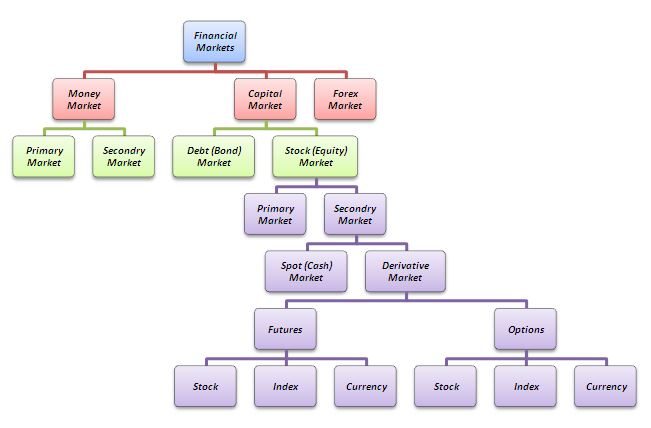
\includegraphics{FigFinancialSystem.jpeg}
\emph{Image from \href{https://1.bp.blogspot.com/}{source}}

\section{Bonds}\label{bonds}

A government or corporation can raise money in the capital markets by
issuing \emph{fixed interest securities (FIS)}, also called \emph{bonds}. Bonds
are a form of medium and long-term securities.

This means that investors will lend money to the issuer (for e.g.~the
government or coporation) and in return will receive fixed interest
payments known as \emph{coupons} at fixed dates plus repayment of the loan at
the end of the term.

\textbf{Note} The loan is usually split into smaller units that can be traded
on a stock exchange. For example, a company raises ฿1,000,000,000 by
issuing 10,000,000 bonds, each one a loan of face value ฿100. These can
be bought and sold on a stock exchange.

\subsection{Characteristics of Bonds}\label{characteristics-of-bonds}

\begin{enumerate}
\def\labelenumi{\arabic{enumi}.}
\item
  The \emph{nominal amount or face value} of a bond is the amount of the
  loan it represents. The nominal amount is usually ฿1,000 (without
  further specific, we will set the nominal amount to be ฿100.)
\item
  The interest payments are called \emph{coupons}, usually expressed as a
  percentage per year of the nominal amount. The rate of interest
  denoted by \(D\) is also known as \emph{coupon rate}. They are always \textbf{in
  arrears}.
\item
  Coupons are usually expressed as the amount of interest payable in a
  year, but are paid half-yearly (twice per year) or quarterly (4
  times per year)
\item
  \emph{Coupon dates} are the dates on which the bond issuer will make
  interest payments.
\item
  Bonds have \emph{maturity dates} at which point the principal amount must
  be paid back in full.
\item
  The loan is repaid or redeemed at the end of the term. The
  redemption amount per 100 nominal is the \emph{redemption rate}, often
  expressed as a percentage.

  A loan is redeemed

  \begin{itemize}
  \item
    at a premium if redemption rate \textgreater{} 100\%
  \item
    at par if redemption rate = 100\%
  \item
    at a discount if redemption rate \textless{} 100\%
  \end{itemize}
\item
  Many corporate and government bonds are publicly traded; others are
  traded only over-the-counter (OTC) or privately between the borrower
  and lender.
\end{enumerate}

\begin{example}
\emph{Each bond of ฿100 nominal value carries coupons of 6\% pa payable
half-yearly.}
\end{example}

\textbf{Solution:} The coupon rate of 6\% pa payable half-yearly means that
bondholders will receive
\[ \frac{6\%}{2} \times 100 = ฿ 3 \text{ every half-year}.\]

\begin{example}
\emph{An investor purchases ฿95 for a 5-year fixed interest bond with face
value (or nominal amount of) ฿100. The bond pays coupon of 6\% pa
half-yearly in arrear and the lump sum equal to the nominal amount in 5
years' time. The cashflows related to the payments of the bond can be
shown as follows:}
\end{example}

\textbf{Solution:} Cashflows are given in the following table.

\begin{longtable}[]{@{}ccccccc@{}}
\toprule\noalign{}
Time (year) & 0 & 0.5 & 1 & 1.5 & \(\ldots\) & 5 \\
\midrule\noalign{}
\endhead
\bottomrule\noalign{}
\endlastfoot
Cashflow & -95 & 3 & 3 & 3 & \(\ldots\) & \(3 + 100\) \\
\end{longtable}

\subsection{Examples of Bonds}\label{examples-of-bonds}

\begin{enumerate}
\def\labelenumi{\arabic{enumi}.}
\tightlist
\item
  \textbf{Domestic Bonds}:

  \begin{itemize}
  \tightlist
  \item
    These are issued in the local currency of the country, such as gilts issued by the UK government and treasury bonds issued by the US government.
  \end{itemize}
\item
  \textbf{Eurobonds}:

  \begin{itemize}
  \tightlist
  \item
    These bonds are issued by an entity outside of its domestic market and are typically denominated in a currency that is different from that of the issuer's home country.
  \end{itemize}
\item
  \textbf{Debenture Bonds}:

  \begin{itemize}
  \tightlist
  \item
    These are long-term securities issued by corporations that are not backed by physical assets or collateral, relying instead on the creditworthiness and reputation of the issuer.
  \end{itemize}
\end{enumerate}

\begin{example}
\protect\hypertarget{exm:exampleBondPrice}{}\label{exm:exampleBondPrice}\emph{A company issues a 10-year bond, to be redeemed at 102\%, with coupon of
6\% pa payable half-yearly in arrears. The nominal amount of each bond is
฿100. What repayments are made?}
\end{example}

\textbf{Solution:} Cashflows are given in the following table.

\begin{longtable}[]{@{}cccccccc@{}}
\toprule\noalign{}
Time (year) & 0 & 0.5 & 1 & 1.5 & \(\ldots\) & 9.5 & 10 \\
\midrule\noalign{}
\endhead
\bottomrule\noalign{}
\endlastfoot
Cashflow & \(P\) & 3 & 3 & 3 & \(\ldots\) & \(3\) & \(3 + 102\) \\
\end{longtable}

Here the bond price in the table above is denoted by \(P\).

The following questions may be asked:

\begin{itemize}
\item
  At what price should be paid by an investor to obtain a net yield of
  \(i\) per annum?
\item
  Given the price of the fixed interest bond, what is the net yield
  per annum will be obtained?
\end{itemize}

\subsection{Bond prices}\label{bond-prices}

Given a yield \(i\%\), the price of a bond can be computed by discounting
all the future payments received net of any tax.

\begin{example}
\protect\hypertarget{exm:exampleBondPrice2}{}\label{exm:exampleBondPrice2}\emph{A tax-exempt investor buy the bond in Example}
\ref{exm:exampleBondPrice} \emph{on its issue date. Calculate the price the
investor should pay to obtain a yield of 9\%.}
\end{example}

\textbf{Solution:} Appplying the Principle of Equivalence: by equate the
present value of the future incomes at 9\% with the unknown price \(P\).

\[P = \frac{6}{2} a^j_{\angl{20}} + 102 (\frac{1}{1.09})^{20},\] where
\(j = (1.09)^{(1/2)} - 1 = 0.044031.\) This gives \(P = 82.44\). It should
be emphasised that the price in this example differs from the nominal
amount of 100.

\begin{example}

\emph{Refer to Examples} \ref{exm:exampleBondPrice} \emph{and}
\ref{exm:exampleBondPrice2}\emph{. After the 10th coupon has been paid, the
investor sells the bond. At that time the market yield on comparable
5-year bonds is 7\% pa effective.}

\begin{enumerate}
\def\labelenumi{\arabic{enumi}.}
\item
  \emph{Calculate the price that he will obtain.}
\item
  \emph{Calculate the yield that the first investor obtains if he paid
  ฿82.44 and received 10 coupon payments of ฿3 each and sold the bond
  after 5 years at the price of ฿97.75.}
\end{enumerate}

\end{example}

\textbf{Solution:}

\begin{enumerate}
\def\labelenumi{\arabic{enumi}.}
\tightlist
\item
  The remaining payments are shown in the table below.
\end{enumerate}

\begin{longtable}[]{@{}
  >{\centering\arraybackslash}p{(\columnwidth - 14\tabcolsep) * \real{0.2812}}
  >{\centering\arraybackslash}p{(\columnwidth - 14\tabcolsep) * \real{0.0781}}
  >{\centering\arraybackslash}p{(\columnwidth - 14\tabcolsep) * \real{0.0781}}
  >{\centering\arraybackslash}p{(\columnwidth - 14\tabcolsep) * \real{0.0781}}
  >{\centering\arraybackslash}p{(\columnwidth - 14\tabcolsep) * \real{0.0781}}
  >{\centering\arraybackslash}p{(\columnwidth - 14\tabcolsep) * \real{0.1562}}
  >{\centering\arraybackslash}p{(\columnwidth - 14\tabcolsep) * \real{0.0781}}
  >{\centering\arraybackslash}p{(\columnwidth - 14\tabcolsep) * \real{0.1719}}@{}}
\toprule\noalign{}
\begin{minipage}[b]{\linewidth}\centering
Time (half-year)
\end{minipage} & \begin{minipage}[b]{\linewidth}\centering
10
\end{minipage} & \begin{minipage}[b]{\linewidth}\centering
11
\end{minipage} & \begin{minipage}[b]{\linewidth}\centering
12
\end{minipage} & \begin{minipage}[b]{\linewidth}\centering
13
\end{minipage} & \begin{minipage}[b]{\linewidth}\centering
\(\ldots\)
\end{minipage} & \begin{minipage}[b]{\linewidth}\centering
19
\end{minipage} & \begin{minipage}[b]{\linewidth}\centering
20
\end{minipage} \\
\midrule\noalign{}
\endhead
\bottomrule\noalign{}
\endlastfoot
Cashflow & \(-\) & 3 & 3 & 3 & \(\ldots\) & \(3\) & \(3 + 102\) \\
\end{longtable}

Working in unit of half-year, we first calculate the effective rate per
half-year, denoted by \(k\), that is equivalent to \(i = 7\%\).

\[ k = (1.07)^{(1/2)} - 1 = 0.034408. \]

The price \(P'\) that he will obtain follows from the following equation.
\[P' = 3 a^k_{\angl{10}} + 102 (\frac{1}{1.07})^{5} = 97.75.\]

\begin{enumerate}
\def\labelenumi{\arabic{enumi}.}
\setcounter{enumi}{1}
\tightlist
\item
  The payments of the investor are shown in the table below.
\end{enumerate}

\begin{longtable}[]{@{}
  >{\centering\arraybackslash}p{(\columnwidth - 14\tabcolsep) * \real{0.2609}}
  >{\centering\arraybackslash}p{(\columnwidth - 14\tabcolsep) * \real{0.1159}}
  >{\centering\arraybackslash}p{(\columnwidth - 14\tabcolsep) * \real{0.0725}}
  >{\centering\arraybackslash}p{(\columnwidth - 14\tabcolsep) * \real{0.0725}}
  >{\centering\arraybackslash}p{(\columnwidth - 14\tabcolsep) * \real{0.0725}}
  >{\centering\arraybackslash}p{(\columnwidth - 14\tabcolsep) * \real{0.1449}}
  >{\centering\arraybackslash}p{(\columnwidth - 14\tabcolsep) * \real{0.0725}}
  >{\centering\arraybackslash}p{(\columnwidth - 14\tabcolsep) * \real{0.1884}}@{}}
\toprule\noalign{}
\begin{minipage}[b]{\linewidth}\centering
Time (half-year)
\end{minipage} & \begin{minipage}[b]{\linewidth}\centering
0
\end{minipage} & \begin{minipage}[b]{\linewidth}\centering
1
\end{minipage} & \begin{minipage}[b]{\linewidth}\centering
2
\end{minipage} & \begin{minipage}[b]{\linewidth}\centering
3
\end{minipage} & \begin{minipage}[b]{\linewidth}\centering
\(\ldots\)
\end{minipage} & \begin{minipage}[b]{\linewidth}\centering
9
\end{minipage} & \begin{minipage}[b]{\linewidth}\centering
10
\end{minipage} \\
\midrule\noalign{}
\endhead
\bottomrule\noalign{}
\endlastfoot
Cashflow & -82.44 & 3 & 3 & 3 & \(\ldots\) & \(3\) & \(3 + 97.75\) \\
\end{longtable}

Let \(i\) denote the yield (per half-year) that the first investor
obtains. Working at time 10, the equation of value of the cashflows is
\[ f(i) = 82.44 (1+i)^{10} - 3 s^i_{\angl{10}} - 97.75 = 0.\] By linear
interpolation, we have \[ f(0.05) = -1.1976, \quad f(0.06) = 10.3451, \]
and hence, the approximate of \(i\) is \(i^* \approx 0.051038\). The annual
yield is then approximately equal to \((1 + 0.051038)^2 - 1 = 10.468\%\)

\textbf{Notes}

\begin{enumerate}
\def\labelenumi{\arabic{enumi}.}
\item
  If the investor is not subject to taxation, the yield is called the
  \emph{gross yield}.
\item
  The yield obtained by holding the bond until redemption is called
  \emph{redemption yield}. This is quoted in financial newspapers.
\item
  If a bond is sold before redemption, the yield that the investor
  obtains is called \emph{realised yield}. This yield depends on both the
  buying and selling prices.
\end{enumerate}

\textbf{Notes}

\begin{enumerate}
\def\labelenumi{\arabic{enumi}.}
\item
  There is an inverse relationship between the bond prices and yields.

  \begin{itemize}
  \tightlist
  \item
    When bond prices rise, the yields associated with those bonds fall.
  \item
    Conversely, when bond prices decrease, yields increase. This relationship occurs because a bond's yield represents the return an investor can expect to receive based on the bond's purchase price and its coupon payments.
  \end{itemize}
\item
  The nominal amount of the loan is just a theoretical figure on which
  the coupon and redemption rates are based.
\item
  The amount of capital a borrower can actually raise on the issue date depends on the price that investors are willing to pay for the future income stream from the bond. This price is influenced by the interplay of supply and demand in the market.
\item
  The investors also consider the \textbf{credit risk} of the borrower. It
  is the risk that they might default on interest and capital
  payments.
\item
  The greater the credit risk, the higher the yield they will require.
\item
  The bonds can be traded on an exchange at any time until it is
  redeemed. The prices will depend on the remaining term to redemption
  and market conditions such as the yields obtainable on other
  investments.
\end{enumerate}

\subsection{No tax}\label{no-tax}

A tax-exempt investor receives the full amount of the coupon and
redemption payments. The price of an \(n\) year fixed interest bond which
pays coupons of \(D\) per annum payable \(p\) thly in arrear and has
redemption amount \(R\) is \[P = D a_{\angln}^{(p)} + R v^n\] at rate \(i\)
per annum.

In practice, we can calculate by using a suitable time period, for
example a period of half a year as shown in the previous examples. Then
the formula can be written as
\[P = \frac{D}{2} a_{\angl{2n}} + R v^{2n}\]

\subsection{Income tax}\label{income-tax}

Suppose an investor is subject to income tax at rate \(t_1\) on the
coupons, which is due at the time that the coupons are paid. Tax will
affect both yields and bond prices. In general, the price of this bond,
an \(n\) year fixed interest bond which pays coupons of \(D\) per annum
payable \(p\) thly in arrear and has redemption amount \(R\) is
\[P = (1 - t_1) D a_{\angln}^{(p)} + R v^n\] at rate \(i\) per annum. Here
the rate is called the \emph{net yield}.

\begin{example}
\emph{An investor liable to income tax at 30\% buys a 15-year fixed interest
bond which is redeemable at par and pays coupons of 8\% pa half-yearly in
arrear. Calculate the price the investor should pay to obtain a net
yield of 9\% pa.}
\end{example}

\textbf{Solution:} Coupon payments after tax are
\[ (1 - t_1) D = (1 - 0.3) \frac{8\%}{2} \times 100 = 2.8.\]

The payments of the investor are shown in the table below.

\begin{longtable}[]{@{}
  >{\centering\arraybackslash}p{(\columnwidth - 14\tabcolsep) * \real{0.2727}}
  >{\centering\arraybackslash}p{(\columnwidth - 14\tabcolsep) * \real{0.0758}}
  >{\centering\arraybackslash}p{(\columnwidth - 14\tabcolsep) * \real{0.0758}}
  >{\centering\arraybackslash}p{(\columnwidth - 14\tabcolsep) * \real{0.0758}}
  >{\centering\arraybackslash}p{(\columnwidth - 14\tabcolsep) * \real{0.0758}}
  >{\centering\arraybackslash}p{(\columnwidth - 14\tabcolsep) * \real{0.1515}}
  >{\centering\arraybackslash}p{(\columnwidth - 14\tabcolsep) * \real{0.0758}}
  >{\centering\arraybackslash}p{(\columnwidth - 14\tabcolsep) * \real{0.1970}}@{}}
\toprule\noalign{}
\begin{minipage}[b]{\linewidth}\centering
Time (half-year)
\end{minipage} & \begin{minipage}[b]{\linewidth}\centering
0
\end{minipage} & \begin{minipage}[b]{\linewidth}\centering
1
\end{minipage} & \begin{minipage}[b]{\linewidth}\centering
2
\end{minipage} & \begin{minipage}[b]{\linewidth}\centering
3
\end{minipage} & \begin{minipage}[b]{\linewidth}\centering
\(\ldots\)
\end{minipage} & \begin{minipage}[b]{\linewidth}\centering
29
\end{minipage} & \begin{minipage}[b]{\linewidth}\centering
30
\end{minipage} \\
\midrule\noalign{}
\endhead
\bottomrule\noalign{}
\endlastfoot
Cashflow & \(P\) & 2.8 & 2.8 & 2.8 & \(\ldots\) & 2.8 & \(2.8 + 100\) \\
\end{longtable}

The price the investor should pay to obtain a net yield of 9\% pa can be
calculated from
\[P = 2.8 a^j_{\angl{30}} + 100 (\frac{1}{1+j})^{30} = 73.59,\] where
where \(j = (1.09)^{(1/2)} - 1 = 0.044031\) per half-year effective.

\subsection{Capital gains tax (CGT)}\label{capital-gains-tax-cgt}

Capital gains tax is a tax levied on the capital gain made on the
redemption of a bond (or the sale of the bond if sold earlier). The
capital gain is simply the difference between

Note that \textbf{capital gain} refers to an increase in a capital asset's
value and is considered to be realized when the asset is sold. A
\textbf{capital loss} is incurred when there is a decrease in the capital
asset value compared to an asset's purchase price.

\begin{example}
\emph{An investor liable to the capital gains tax at 20\% purchases two bonds}

\begin{itemize}
\item
  \emph{Bond A for the price of ฿102 and}
\item
  \emph{Bond B for the price of ฿98.}
\end{itemize}

\emph{Calculate the capital gains tax on each bond if the investor sells them
both one year later for ฿100 each.}
\end{example}

\textbf{Solution:}

\begin{itemize}
\item
  Bond A: Tax payment is \(0.2 \times \max\{100 - 102,0 \} = 0\) (i.e.
  capital loss)
\item
  Bond B: Tax payment is \(0.2 \times \max\{100 - 98,0 \} = 0.4\) (i.e.
  capital gain)
\end{itemize}

Here we assume that no `relief', i.e.~we cannot add the two bonds
together and say we bought the two bonds for ฿200 and sold the bonds for
฿200.

\textbf{Notes}

\begin{enumerate}
\def\labelenumi{\arabic{enumi}.}
\item
  Similar to income tax, the price of the bond is then calculated on
  the net redemption received after tax has been deducted.
\item
  When the purchase and sale (or redemption) prices are known, it it
  easy to calculate the yield.
\item
  In contrast, as the price depends on whether there is a capital gain
  and the capital gain depends on the price, it is not easy to
  calculate the price for a given redemption yield. There is a test to
  determine whether CGT is payable.
\end{enumerate}

\begin{example}

\emph{An investor liable to the capital gains tax at 20\% purchases a 10-year
bond with an annual coupon of 8\% pa payable yearly in arrear, to be
redeemed at par.}

\begin{enumerate}
\def\labelenumi{\arabic{enumi}.}
\item
  \emph{Calculate the redemption yield the investor obtain if the price is
  ฿96 per ฿100 nominal.}
\item
  \emph{What price should the investor pay to obtain a yield of 7\% pa
  effective?} (see note below)
\item
  \emph{What price should the investor pay to obtain a yield of 9\% pa
  effective?}\\
\end{enumerate}

\end{example}

\textbf{Solution:}

\begin{enumerate}
\def\labelenumi{\arabic{enumi}.}
\tightlist
\item
  The bond is redeemed at par. Therefore, the redemption amount is 100
  THB which is greater than the bond price, and the capital gain tax
  is \textbf{payable}.
\end{enumerate}

The payments of the investor are shown in the table below.

\begin{longtable}[]{@{}
  >{\centering\arraybackslash}p{(\columnwidth - 14\tabcolsep) * \real{0.1781}}
  >{\centering\arraybackslash}p{(\columnwidth - 14\tabcolsep) * \real{0.0685}}
  >{\centering\arraybackslash}p{(\columnwidth - 14\tabcolsep) * \real{0.0685}}
  >{\centering\arraybackslash}p{(\columnwidth - 14\tabcolsep) * \real{0.0685}}
  >{\centering\arraybackslash}p{(\columnwidth - 14\tabcolsep) * \real{0.0685}}
  >{\centering\arraybackslash}p{(\columnwidth - 14\tabcolsep) * \real{0.1370}}
  >{\centering\arraybackslash}p{(\columnwidth - 14\tabcolsep) * \real{0.0685}}
  >{\centering\arraybackslash}p{(\columnwidth - 14\tabcolsep) * \real{0.3425}}@{}}
\toprule\noalign{}
\begin{minipage}[b]{\linewidth}\centering
Time (year)
\end{minipage} & \begin{minipage}[b]{\linewidth}\centering
0
\end{minipage} & \begin{minipage}[b]{\linewidth}\centering
1
\end{minipage} & \begin{minipage}[b]{\linewidth}\centering
2
\end{minipage} & \begin{minipage}[b]{\linewidth}\centering
3
\end{minipage} & \begin{minipage}[b]{\linewidth}\centering
\(\ldots\)
\end{minipage} & \begin{minipage}[b]{\linewidth}\centering
9
\end{minipage} & \begin{minipage}[b]{\linewidth}\centering
10
\end{minipage} \\
\midrule\noalign{}
\endhead
\bottomrule\noalign{}
\endlastfoot
Cashflow & -96 & 8 & 8 & 8 & \(\ldots\) & 8 & 8 + 100 - 0.2(100 - 96) \\
\end{longtable}

Let \(i\) denote the yield per year that the first investor obtains.
Working at time 10, the equation of value of the cashflows is
\[ f(i) =  -96 (1+i)^{10} + 8 s^i_{\angl{10}} +  99.2 = 0.\] By linear
interpolation, we have \[ f(0.08) = 7.836, \quad f(0.09) = -6.523, \]
and hence, the approximate of \(i\) is \(i^* \approx 0.08546 = 8.546\%\).

\begin{enumerate}
\def\labelenumi{\arabic{enumi}.}
\setcounter{enumi}{1}
\tightlist
\item
  We know that \(P = 96\) is equivalent to yield approximately equal to
  \(8.546\%\).
\end{enumerate}

To obtain a yield of \(7\%\), this should imply that \(P > 96\). If
\(P \ge R = 100\), no CGT is payable. This would change the equation we
need to calculate the bond price. Two cases to be considered are

\begin{itemize}
\item
  \textbf{CGT is payable:} The equation of value is
  \[ P = 8 a^i_{\angl{10}} +  99.2\cdot (1+i)^{-10}, \quad i = 7\%\]
\item
  \textbf{CGT is not payable:} The equation of value is
  \[ P = 8 a^i_{\angl{10}} +  100\cdot (1+i)^{-10}, \quad i = 7\%\]
\end{itemize}

\textbf{Note} In this example, we can guess whether CGT is payable because we
have calculated the price to yield 8.546\% from the above question. Then
we can use the appropriate equation to calculate the bond price and
check whether or not our initial guess was correct.

According to the note, let us guess that \(P > 100\), i.e.~CGT is \textbf{not}
payable.

\[ P = 8 a^i_{\angl{10}} +  100\cdot (1+i)^{-10}, \quad i = 7\%,\] which
implies that \(P = 107.02 > 100\). So our initial guess was correct and
CGT is \textbf{not} payable.

\begin{enumerate}
\def\labelenumi{\arabic{enumi}.}
\setcounter{enumi}{2}
\tightlist
\item
  Here \(9\% > 8.546\%\). Let us guess that \(P < 100\), i.e.~CGT is
  payable.
  \[ P = 8 a^i_{\angl{10}} +  99.2\cdot (1+i)^{-10}, \quad i = 7\%,\]
  which implies that \(P = 92.99 < 100\). So our initial guess was
  correct and CGT is payable.
\end{enumerate}

\subsection{Capital Gains Test}\label{capital-gains-test}

Consider an \(n\)-year fixed-interest security that pays coupons of \(D\) per annum, payable \(p\)-thly in arrears, and has a redemption amount of \(R\). An investor, liable to income tax at a rate of \(t_1\) (due at the same time the coupons are paid), purchases the bond at a price of \(P'\). If \(R > P'\), then there is a capital gain. We have:

\[
R > (1 - t_1) D a_{\angln}^{(p)} + R v^n
\]

This simplifies to:

\[
R(1 - v^n) > (1 - t_1) D a_{\angln}^{(p)} 
\]

\[
R(1 - v^n) > (1 - t_1) D \frac{1 - v^n }{i^{(p)}} 
\]

Thus,

\[
R > (1 - t_1) \frac{D }{i^{(p)}} 
\]

This leads to the conclusion that:

\[
i^{(p)} > (1 - t_1) \frac{D}{R} 
\]

An intuitive way to think about this is that the overall return on a bond comes from both the coupons and any capital gain. If the required return is greater than the net coupons we receive, then we must be receiving more than we initially paid, indicating a capital gain.

\section{Inflation}\label{inflation}

Inflation is a measure of the rate of change in the price of consumer
goods and services, such as food and beverages, transportation and
housing.

\begin{itemize}
\item
  In Thailand or US, it is measured with reference to a \textbf{consumer
  price index} (or CPI). In UK, it is measured in terms of \textbf{retail
  price index} (RPI).
\item
  Bureau of Trade and Economic Indices reports the CPI on a monthly
  basis.
\item
  High inflation means that prices increase quickly and hence \textbf{the
  purchasing power} significantly decreases.
\end{itemize}

Let \(Q(t)\) be the CPI at time \(t\). Then the rate of inflation per year
denoted by \(q(t)\) is \[q(t) = \frac{Q(t)}{Q(t-1)} - 1.\] The average
inflation rate per year between time \(s\) and \(t\), denoted by \(\bar{q}\),
satisfies \[(1 + \bar{q})^{t-s} = \frac{Q(t)}{Q(s)},\] and hence
\[\bar{q} = \left( \frac{Q(t)}{Q(s)}  \right)^{1/(t-s)} - 1.\]

\begin{example}
\emph{A set of goods costs ฿98.25 in January 2013 and ฿101.44 in January
2018. Calculate the average inflation rate} \(\bar{q}\) over this period.
\end{example}

\textbf{Solution:} The increase from Jan 2013 to Jan 2018 (5 years) is
\[\frac{101.44}{98.25}  - 1 =   0.032.\] The average of inflation rate
\(\bar{q}\) is given by \[(1  + \bar{q})^5 = 1.032.\] Therefore
\(\bar{q} = 0.64\%\).

Therefore, ฿1 in January 2013 buys as much as ฿1.032 in January 2018.

The following table shows the monthly consumer price indices from
January 2011 to December 2019. Source: \url{http://www.price.moc.go.th/}

\begin{longtable}[]{@{}
  >{\raggedright\arraybackslash}p{(\columnwidth - 24\tabcolsep) * \real{0.0588}}
  >{\raggedright\arraybackslash}p{(\columnwidth - 24\tabcolsep) * \real{0.0784}}
  >{\raggedright\arraybackslash}p{(\columnwidth - 24\tabcolsep) * \real{0.0784}}
  >{\raggedright\arraybackslash}p{(\columnwidth - 24\tabcolsep) * \real{0.0784}}
  >{\raggedright\arraybackslash}p{(\columnwidth - 24\tabcolsep) * \real{0.0784}}
  >{\raggedright\arraybackslash}p{(\columnwidth - 24\tabcolsep) * \real{0.0784}}
  >{\raggedright\arraybackslash}p{(\columnwidth - 24\tabcolsep) * \real{0.0784}}
  >{\raggedright\arraybackslash}p{(\columnwidth - 24\tabcolsep) * \real{0.0784}}
  >{\raggedright\arraybackslash}p{(\columnwidth - 24\tabcolsep) * \real{0.0784}}
  >{\raggedright\arraybackslash}p{(\columnwidth - 24\tabcolsep) * \real{0.0784}}
  >{\raggedright\arraybackslash}p{(\columnwidth - 24\tabcolsep) * \real{0.0784}}
  >{\raggedright\arraybackslash}p{(\columnwidth - 24\tabcolsep) * \real{0.0784}}
  >{\raggedright\arraybackslash}p{(\columnwidth - 24\tabcolsep) * \real{0.0784}}@{}}
\caption{\label{tab:tableCPI} The monthly consumer price indices from January 2011
to December 2019.}\tabularnewline
\toprule\noalign{}
\begin{minipage}[b]{\linewidth}\raggedright
Year
\end{minipage} & \begin{minipage}[b]{\linewidth}\raggedright
1
\end{minipage} & \begin{minipage}[b]{\linewidth}\raggedright
2
\end{minipage} & \begin{minipage}[b]{\linewidth}\raggedright
3
\end{minipage} & \begin{minipage}[b]{\linewidth}\raggedright
4
\end{minipage} & \begin{minipage}[b]{\linewidth}\raggedright
5
\end{minipage} & \begin{minipage}[b]{\linewidth}\raggedright
6
\end{minipage} & \begin{minipage}[b]{\linewidth}\raggedright
7
\end{minipage} & \begin{minipage}[b]{\linewidth}\raggedright
8
\end{minipage} & \begin{minipage}[b]{\linewidth}\raggedright
9
\end{minipage} & \begin{minipage}[b]{\linewidth}\raggedright
10
\end{minipage} & \begin{minipage}[b]{\linewidth}\raggedright
11
\end{minipage} & \begin{minipage}[b]{\linewidth}\raggedright
12
\end{minipage} \\
\midrule\noalign{}
\endfirsthead
\toprule\noalign{}
\begin{minipage}[b]{\linewidth}\raggedright
Year
\end{minipage} & \begin{minipage}[b]{\linewidth}\raggedright
1
\end{minipage} & \begin{minipage}[b]{\linewidth}\raggedright
2
\end{minipage} & \begin{minipage}[b]{\linewidth}\raggedright
3
\end{minipage} & \begin{minipage}[b]{\linewidth}\raggedright
4
\end{minipage} & \begin{minipage}[b]{\linewidth}\raggedright
5
\end{minipage} & \begin{minipage}[b]{\linewidth}\raggedright
6
\end{minipage} & \begin{minipage}[b]{\linewidth}\raggedright
7
\end{minipage} & \begin{minipage}[b]{\linewidth}\raggedright
8
\end{minipage} & \begin{minipage}[b]{\linewidth}\raggedright
9
\end{minipage} & \begin{minipage}[b]{\linewidth}\raggedright
10
\end{minipage} & \begin{minipage}[b]{\linewidth}\raggedright
11
\end{minipage} & \begin{minipage}[b]{\linewidth}\raggedright
12
\end{minipage} \\
\midrule\noalign{}
\endhead
\bottomrule\noalign{}
\endlastfoot
2011 & 91.93 & 92.3 & 92.75 & 94.03 & 94.35 & 94.47 & 94.64 & 95.05 & 94.73 & 94.91 & 95.12 & 94.66 \\
2012 & 95.03 & 95.38 & 95.95 & 96.35 & 96.73 & 96.89 & 97.22 & 97.61 & 97.93 & 98.06 & 97.71 & 98.09 \\
2013 & 98.25 & 98.46 & 98.52 & 98.68 & 98.92 & 99.07 & 99.17 & 99.16 & 99.32 & 99.49 & 99.59 & 99.73 \\
2014 & 100.15 & 100.39 & 100.6 & 101.1 & 101.51 & 101.4 & 101.32 & 101.23 & 101.06 & 100.96 & 100.84 & 100.33 \\
2015 & 99.74 & 99.86 & 100.03 & 100.05 & 100.22 & 100.32 & 100.25 & 100.03 & 99.98 & 100.18 & 99.86 & 99.47 \\
2016 & 99.21 & 99.36 & 99.57 & 100.11 & 100.68 & 100.71 & 100.36 & 100.32 & 100.36 & 100.52 & 100.46 & 100.59 \\
2017 & 100.75 & 100.79 & 100.33 & 100.49 & 100.64 & 100.66 & 100.53 & 100.64 & 101.22 & 101.38 & 101.45 & 101.37 \\
2018 & 101.44 & 101.21 & 101.12 & 101.57 & 102.14 & 102.05 & 102.00 & 102.27 & 102.57 & 102.63 & 102.40 & 101.73 \\
2019 & 101.71 & 101.95 & 102.37 & 102.82 & 103.31 & 102.94 & 103.00 & 102.80 & 102.90 & 102.74 & 102.61 & 102.62 \\
\end{longtable}

Figure \ref{fig:figCPI} shows the monthly consumer price indices from
January 2011 to December 2019.

\begin{figure}

{\centering 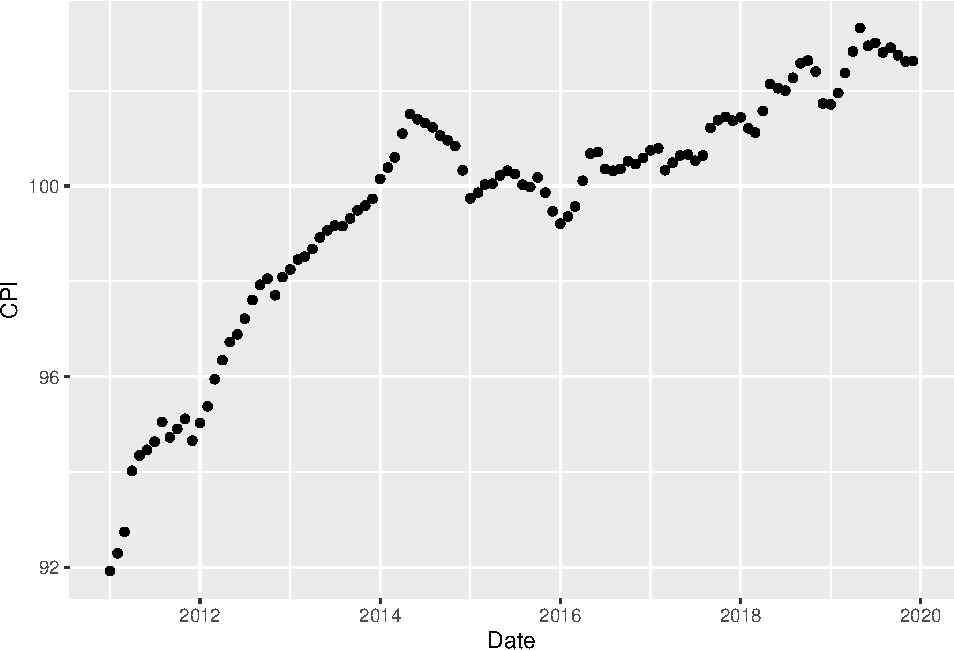
\includegraphics{SCMA266Bookdownproj_files/figure-latex/figCPI-1} 

}

\caption{The monthly consumer price indices from January 2011 to December 2019}\label{fig:figCPI}
\end{figure}

\begin{example}

\emph{An investment contract made on January 2018 promises to pay an investor
of ฿10,000 in 5 years' time. Assume the average inflation rate at}
\(\bar{q} = 0.64\%\) for the next 5 years.

\emph{If a bowl of noodles costs ฿100 in 2018, then ฿10,000 could buy 100
bowls. How many bowls of noodles would the payment of ฿10,000 buy in the
next 5 years?}

\emph{\textbf{Solution:} In Jan 2018, ฿100 buys as much as} \(100 (1.0064)^5 =\)
฿103.2 in Jan 2023.

\emph{So ฿10000 in Jan 2023 could buy}
\[\frac{10000}{103.2} \approx 96 \text{ bowls}.\] Notice that we divide
by \((1 + \bar{q})^5\) to calculate how much your money is worth at the
end of the next five years.

\begin{itemize}
\item
  \emph{The quantity of goods that can be bought with 10,000 in January
  2023 reduces from 100 to 96 bowls.}
\item
  \emph{The effect of inflation results in the reduction of the purchasing
  power of a unit of money in January 2023 compared to that in
  January 2018.}
\item
  \emph{The amount of ฿10,000 is referred to as the \textbf{monetary} (or
  \textbf{nominal}) payment in 5 years. This is the amount of money that
  change hands.}
\item
  \emph{The \textbf{real payment of ฿10,000 (due at time 5 years) in time 0
  unit} is} \[\begin{aligned}
  10000 \frac{Q(0)}{Q(5)} &=  10000  \frac{1}{(1.0064)^5} \\
                           &=  9686.05.\end{aligned}\] Here we have
  less purchasing power with your money at the end of the five years
  than you had at the start of the year.
\item
  \emph{The real payment (in time 0) is the purchase power of 10,000 paid
  in 5 years relative to today. \textbf{It is the amount of cash in hand at
  the end of the period reduced for the effects of inflation}.}
\item
  \emph{In general, ฿X at time} \(t\) has the purchasing power relative to
  time \(s\) of \[X \cdot \frac{Q(s)}{Q(t)}.\]
\end{itemize}

\end{example}

\subsection{Real rates of interest}\label{real-rates-of-interest}

The rate of interest which is calculated using monetary payments is
called a \textbf{money (or monetary or nominal) rate of interest}.

The \textbf{real rate of interest} is calculated using real payments.

\begin{example}

\emph{An investor deposits 100 at time 0 and receives 120 after one year.}

\begin{itemize}
\item
  \emph{The monetary rate of interest effective is}
  \[\frac{120}{100} - 1 = 20\%.\]
\item
  \emph{Suppose that the inflation rate over this one year period is 4\%.
  Calculate the real payment of 120 at time 1 and the real rate of
  interest. After adjusting for the inflation rate, the real rate of
  interest can be calculated by first expressing both payments in
  units of the same purchasing power.}

  \begin{itemize}
  \item
    \emph{In term of time 0 money unit, the transaction is represented
    by}

    \emph{Here, the real payment of 120 due in 1 year in terms of time 0
    unit is} \(\displaystyle{120 \cdot \frac{1}{1.04} = 115.38}\).
    Hence the real rate of interest is 15.38\%.
  \item
    \emph{In term of time 1 money unit, the transaction is represented
    by}

    \emph{Similarly, we instead calculate the real payment of 100
    relative to time 1, which gives} \(100 \cdot 1.04 = 104\). The
    real rate of interest is \[\frac{120}{104} - 1 = 15.38\%,\]
    which is the same as the previous case.
  \end{itemize}
\end{itemize}

\end{example}

\subsection{Real yields}\label{real-yields}

It is often useful to look at the rate of return earned on an investment
after taking into account of inflation. As analogous to the real rate of
interest, a \textbf{real yield} is calculated using real payments, which can
be obtained by expressing payments in units of the same purchasing power
\textbf{at some specific date}.

\begin{example}
\emph{A 5-year bond with nominal value of ฿100 was issued in January 2013.
The coupon rate was 8\% p.a. payable yearly in arrears. Redemption was at
par after 5 years. The bond was issued at 100\%. Calculate the yield to a
non-tax paying investor}

\begin{enumerate}
\def\labelenumi{\arabic{enumi}.}
\item
  \emph{in monetary terms \textbf{Solution:}}

  \emph{The transaction together with the inflation indices} \(Q(t)\) at time
  \(t\) is shown as follows:

  \emph{Clearly, the monetary rate of return on this transaction is 8\%.
  This is because the investor receives the interest payment of ฿8 at
  the end of each year plus the initial capital of ฿100 at the end of
  five years.}

  \emph{Alternatively, one can solve for the monetary rate of return from
  the following equation of value}
  \[f(i) = -100 + 8 a^i_{\actuarialangle{5}} + 100\frac{1}{(1+i)^5} = 0.\]
\item
  \emph{in real terms with reference to the CPI.}

  \emph{Taking into account of the inflation rates, we calculate the real
  payment in term of time 0 unit by dividing the monetary amounts by
  the \textbf{proportional} increase in the inflation index from 0 to} \(t\).
\end{enumerate}

\begin{longtable}[]{@{}
  >{\centering\arraybackslash}p{(\columnwidth - 12\tabcolsep) * \real{0.0686}}
  >{\centering\arraybackslash}p{(\columnwidth - 12\tabcolsep) * \real{0.0490}}
  >{\centering\arraybackslash}p{(\columnwidth - 12\tabcolsep) * \real{0.1716}}
  >{\centering\arraybackslash}p{(\columnwidth - 12\tabcolsep) * \real{0.1716}}
  >{\centering\arraybackslash}p{(\columnwidth - 12\tabcolsep) * \real{0.1716}}
  >{\centering\arraybackslash}p{(\columnwidth - 12\tabcolsep) * \real{0.1716}}
  >{\centering\arraybackslash}p{(\columnwidth - 12\tabcolsep) * \real{0.1716}}@{}}
\toprule\noalign{}
\begin{minipage}[b]{\linewidth}\centering
Time
\end{minipage} & \begin{minipage}[b]{\linewidth}\centering
0
\end{minipage} & \begin{minipage}[b]{\linewidth}\centering
1
\end{minipage} & \begin{minipage}[b]{\linewidth}\centering
2
\end{minipage} & \begin{minipage}[b]{\linewidth}\centering
3
\end{minipage} & \begin{minipage}[b]{\linewidth}\centering
4
\end{minipage} & \begin{minipage}[b]{\linewidth}\centering
5
\end{minipage} \\
\midrule\noalign{}
\endhead
\bottomrule\noalign{}
\endlastfoot
Year & 2013 & 2014 & 2015 & 2016 & 2017 & 2018 \\
Cashflow & -100 & 8 & 8 & 8 & 8 & 8 + 100 \\
CPI & 98.25 & 100.15 & 99.74 & 99.21 & 100.75 & 101.44 \\
Real
value
of cashflow
at
\(t = 0\) & -100 & \(8 \cdot \frac{98.25}{100.15}\)
= 7.85 & \(8 \cdot \frac{98.25}{99.74}\)
= 7.88 & \(8 \cdot \frac{98.25}{99.21}\)
= 7.91 & \(8 \cdot \frac{98.25}{100.75}\)
= 7.80 & \(8 \cdot \frac{98.25}{101.44}\) \textbar{}
= 104.60 \\
\end{longtable}

\emph{The real yield} \(i'\) p.a. effective solve the equation of value as
follows:
\[f(i') = -100 + 7.85 v  + 7.88v^2 + 7.91v^3 + 7.80v^6 + 104.6v^5 = 0,\]
which gives \(i' \approx 7.30\%\) by the linear interpolation.
\end{example}

In general, the real yield \(i'\) for a series of cashflows
\(C(t_1), C(t_2), \ldots, C(t_n)\), given associated inflation index
\(Q(t_k)\) for \(k = 1, \ldots, n\), can be obtained in terms of time 0
money units as
\[\sum_{k=1}^n C(t_k) \frac{Q(0)}{Q(t_k)} \frac{1}{(1 + i')^{t_k}} = 0.\]
This is equivalent to
\[\sum_{k=1}^n C(t_k) \frac{1}{Q(t_k)} \frac{1}{(1 + i')^{t_k}} = 0.\]
Therefore, \textbf{the real yield is independent of the date the payment units
are adjusted to}.

\subsection{Calculating real yields given constant inflation assumptions}\label{calculating-real-yields-given-constant-inflation-assumptions}

For future cashflows, the inflation index will not be known. Suppose we
assume a constant rate of inflation \(q\) p.a. The cashflows \(C(t_k)\) at
time \(t_k\) have the purchasing power at time 0 (or real payments
relative to time 0) \[\begin{aligned}
    C(t_k) \cdot \frac{Q(0)}{Q(t_k)} &=     C(t_k) \cdot \frac{Q(0)}{Q(0)(1+q)^{t_k}}  =  C(t_k) \cdot \frac{1}{(1+q)^{t_k}} , \quad k = 1, \ldots, n.\end{aligned}\]
The relation between the real yield \(i'\), the constant rate of inflation
\(q\) and the monetary yield \(i\) can be obtained as follows: From the
equation of value, \[\begin{aligned}
    0   &= \sum_{k=1}^n C(t_k) \frac{Q(0)}{Q(t_k)} \frac{1}{(1 + i')^{t_k}} \\
        &=  \sum_{k=1}^n C(t_k)  \cdot \frac{1}{(1+q)^{t_k}}\cdot \frac{1}{(1 + i')^{t_k}}\end{aligned}\]
With no inflation adjustment, the monetary rate of return \(i\) satisfies
\[0 =  \sum_{k=1}^n C(t_k)  \cdot \frac{1}{(1+i)^{t_k}}.\] Therefore, if
\textbf{we assume a constant rate of inflation} \(q\) p.a., then the following
relation holds: \[(1 +i) = ( 1 + q)(1+i').\] This provides the
relationship between the real yield \(i'\), the monetary yield \(i\) and the
inflation rate \(q\).

\subsection{Index-linked securities}\label{index-linked-securities}

An index-linked security is an investment security in which interest
payments and the redemption are adjusted in line with inflation index
values by linking the payments to the Consumer Price Index (CPI). The
reasons for these types of security are

\begin{itemize}
\item
  to protect investors against inflation risk, and
\item
  to help pension funds to provide index-link benefits so that the
  index-link liability can be matched with the index-link asset.
\end{itemize}

\begin{example}
\emph{Consider an index-link bond of a nominal of ฿100 issued at time} \(t_0\),
bearing an annual coupon of \(C\%\) payable \(m\) times a year and a
redemption is at \(R\%\). Then per ฿100 nominal, the monetary amount
(actual cashflow) of an interest payment \(D(t_k)\) at time \(t_k\) is

\emph{The monetary amount of the redemption amount at time} \(t_n\) is
\end{example}

\begin{example}
\protect\hypertarget{exm:exampleILB}{}\label{exm:exampleILB}\emph{An investor purchased a 3-year index-linked bond in January 2015. The
investor received payments at the end of each year plus a final
redemption amount, all of which were adjusted in line with the CPI
values reported in Table} \ref{tab:tableCPI}\emph{. Calculate the actual
payments received by the investor.}
\end{example}

\textbf{Note} In practice, due to delays in calculating the index, the
payments (or cashflows) will be adjusted based on the inflation index
value from an earlier period.

Let \(s\) denote the indexation time lag. The payments are adjusted with
reference to inflation index value at time \(s\) (months) before the
payment is made. Then the monetary amount of an interest payment
\(D(t_k)\) per ฿100 nominal at time \(t_k\) is
\[\displaystyle D(t_k) = 100 \frac{C}{m} \cdot \frac{Q(t_k - \frac{s}{12})}{Q(t_0 - \frac{s}{12})}\]
and the monetary amount of redemption at time \(t_n\) is
\[D(t_n) = 100 R \cdot \frac{Q(t_n - \frac{s}{12})}{Q(t_0 - \frac{s}{12})}.\]
The term \(Q(t_0 - \frac{s}{12})\) is called the base inflation figure
(the base CPI figure).

\begin{example}
\emph{Repeat Example}\ref{exm:exampleILB} \emph{for a 3-year index linked bond.
The indexation adjustments are made according to the CPI three months
before each payment, i.e.} \(s = 3\) months.
\end{example}

\begin{example}
\protect\hypertarget{exm:exampleILB2}{}\label{exm:exampleILB2}

\emph{In January 2015, the government issued an index-linked bond of term 10
years. Coupons are payable half-yearly in arrears, and the annual
nominal coupon rate is 4\%. The coupons and redemption amount are
adjusted with reference to the inflation index value 3 months before the
payment is made.}

\emph{Assume the constant inflation rate from February 2018 is 2\% p.a.}

\begin{enumerate}
\def\labelenumi{\arabic{enumi}.}
\item
  \emph{Find the base CPI figure (i.e.~it is the October 2014 CPI which is
  3 months before the issue date).}
\item
  \emph{Calculate the actual payments received by the investor.}
\item
  \emph{Assume that the price of ฿100 nominal of this index-linked bond in
  January 2018 (after the January 2018 coupon payment) is ฿ .
  Calculate the monetary yield that an investor who purchased the bond
  in January 2018 (after the January 2018 coupon payment) will
  obtained.}
\item
  \emph{Calculate the real yield for this investor under the above
  assumptions.}
\end{enumerate}

\end{example}

\chapter{Tutorials}\label{tutorials}

\section{Tutorial 1}\label{tutorial-1}

\begin{enumerate}
\def\labelenumi{\arabic{enumi}.}
\item
  Calculate the following accumulation:

  \begin{enumerate}
  \def\labelenumii{\arabic{enumii}.}
  \item
    Accumulate \$5,000 for 4 years at 7.5\% per annum effective.
  \item
    Accumulate \$800 for 2.7 years at 3\% per quarter-year effective.
  \item
    Accumulate \$10,000 for 27 months at 4.25\% per half-year
    effective.
  \end{enumerate}
\item
  Calculate the present values on 1 January 2015 of the following
  payments at the given rates of interest:

  \begin{enumerate}
  \def\labelenumii{\arabic{enumii}.}
  \item
    \$1,000 on 1 January 2016, at 7.5\% per annum effective.
  \item
    \$100 on 1 October 2016, at 3\% per quarter-year effective.
  \item
    \$10,000 on 1 April 2016, at 4.25\% per half-year effective.
  \end{enumerate}
\item
  \begin{enumerate}
  \def\labelenumii{\arabic{enumii}.}
  \item
    If the effective rate of interest is 4\% per annum, calculate the
    effective rate of interest per month?
  \item
    If the effective rate of interest is 6.5\% per half-year,
    calculate the effective rate of interest per quarter-year?
  \end{enumerate}
\item
  The effective rate of interest per annum was 4\% during 2015, 5\%
  during 2016 and 6\% thereafter.

  \begin{enumerate}
  \def\labelenumii{\arabic{enumii}.}
  \item
    Calculate the accumulation of \$500 from 1 January 2015 to 1
    January 2018.
  \item
    Calculate the accumulation of \$2000 from 1 April 2015 to 1
    October 2017.
  \item
    Calculate the accumulation factor from 1 January 2015 to 1
    January 2018.
  \end{enumerate}
\item
  You deposit \$ 3000 to an account that earn 2.5\% compounded
  annually. How much will you have in three years?
\item
  A person borrows a sum of \$5,000 and agrees to pay this back at the
  end of 1 year with interest calculated at an effective rate of 10\%
  per annum. Calculate the amount to be repaid for the loan.
\item
  You want to have \$1000 in 2 years and \$2000 in 4 years. How much
  should you deposit now into an account earning the effective rate of
  5.75\% semiannually?
\item
  Katy deposits 100 into a saving account which pays interest at \(i\)
  \textbf{per quarter} effective.

  At the same time, Taylor deposits 500 into a different saving
  account which pays a simple interest at an annual rate of \(i\).

  During the last 3 months of the 4th year, they both earn the same
  amount of interest. Calculate \(i\).
\item
  An ordinary annuity is a series of equal payments made at the end of
  consecutive periods over a fixed length of time. Draw a timeline for
  the following annuity having cashflow of 1 unit at the end of each
  of the next n time units.
\item
  Draw a timeline to illustrate this insurance benefit: Whole Life
  Insurance - payable immediately on death - has following conditions:

  \begin{itemize}
  \item
    death benefit (sum insured) of 1
  \item
    payable immediately on the death
  \item
    of an individual currently aged x
  \item
    for death occurring any time in the future.
  \end{itemize}
\item
  (Excel) It is a good exercise to check whether the Excel worksheet
  you have developed so far for calculating the present value and
  future value can be applied to the questions in this Tutorial. What
  would you do to improve the Excel worksheet that can be applied to a
  more general scenario?
\end{enumerate}

\section{Tutorial 2}\label{tutorial-2}

\begin{enumerate}
\def\labelenumi{\arabic{enumi}.}
\item
  Starting at 1 January 2015, the effective rate of interest per annum
  was 3\% per quarter-year for 9 months, 4\% per half-year for 15 months
  and and 2\% per month thereafter.

  \begin{enumerate}
  \def\labelenumii{\arabic{enumii}.}
  \item
    Calculate the accumulation factor from 1 January 2015 to 1
    January 2018.
  \item
    Calculate the accumulation of \$5,000 from 1 July 2015 to 1
    October 2017.
  \item
    Calculate the accumulation of \$100 from 1 March 2016 to 1
    August 2018.
  \item
    Calculate the present value at 1 January 2015 of \$ 25,000
    receivable on 1 July 2016.
  \item
    Calculate the present value at 1 April 2015 of \$ 8,000
    receivable on 1 October 2017.
  \item
    Calculate the discount factor from 1 July 2015 to 1
    October 2016.
  \end{enumerate}
\item
  The effective rate of interest is 7.25\% per time unit. Cashflows are
  shown in the following time line.

  \begin{enumerate}
  \def\labelenumii{\arabic{enumii}.}
  \item
    Calculate the accumulation at time time t = 4 units of these
    cashflows.
  \item
    Calculate the accumulation at time time t = 8 units of these
    cashflows.
  \item
    Calculate the present value at time time t = 0 units of these
    cashflows.
  \end{enumerate}
\end{enumerate}

\begin{center}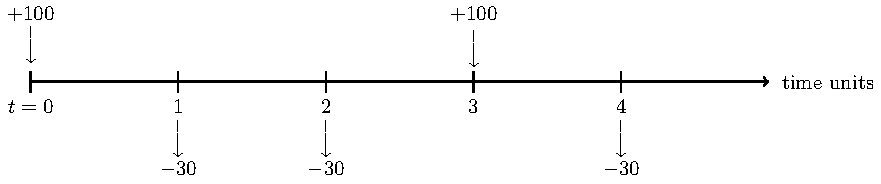
\includegraphics{SCMA266Bookdownproj_files/figure-latex/tikz-exam1-1} \end{center}

\begin{enumerate}
\def\labelenumi{\arabic{enumi}.}
\setcounter{enumi}{2}
\item
  The effective rate of interest is 6\% per time unit. Cashflows are
  shown in the following time line.

  \begin{enumerate}
  \def\labelenumii{\arabic{enumii}.}
  \item
    Calculate the accumulation at time time t = 5 units of these
    cashflows.
  \item
    Calculate the value at time time t = 2 units of these cashflows.
  \item
    Calculate the present value at time time t = 0 units of these
    cashflows.
  \end{enumerate}
\end{enumerate}

\begin{center}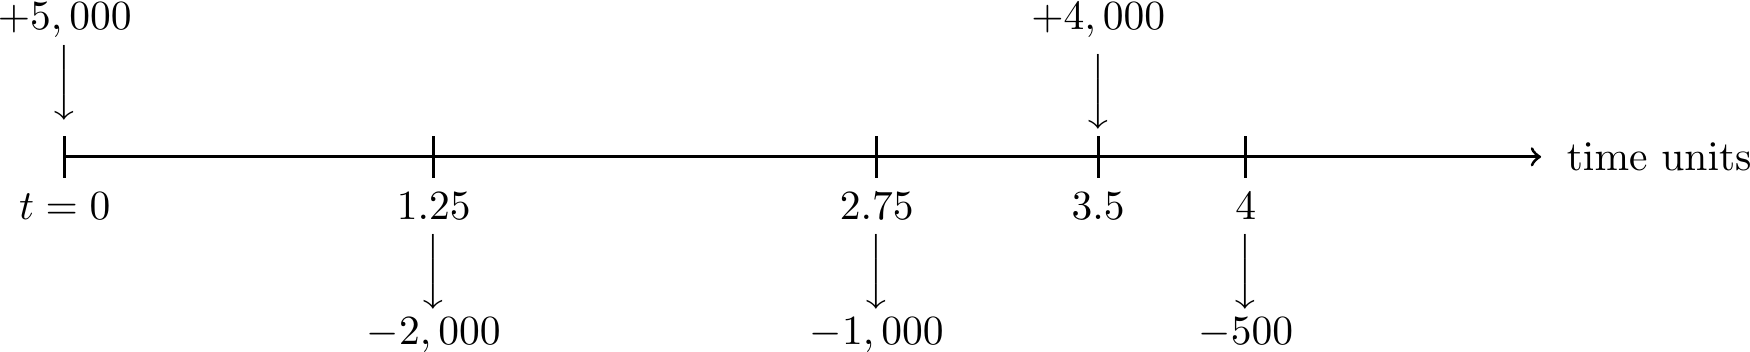
\includegraphics{SCMA266Bookdownproj_files/figure-latex/tikz-exam2-1} \end{center}

\begin{enumerate}
\def\labelenumi{\arabic{enumi}.}
\setcounter{enumi}{3}
\item
  The effective rate of interest per annum was 4\% during 2015, 3\% per
  half-year until 1 October 2017 and 1.5\% per month thereafter.
  Cashflows are shown in the following time line.

  \begin{enumerate}
  \def\labelenumii{\arabic{enumii}.}
  \item
    Calculate the accumulation on 1/1/2019 of these cashflows.
  \item
    Calculate the present value on 1/1/2015 of these cashflows.
  \item
    Calculate the value at time time 1/7/2017 of these cashflows.
  \end{enumerate}
\end{enumerate}

\begin{center}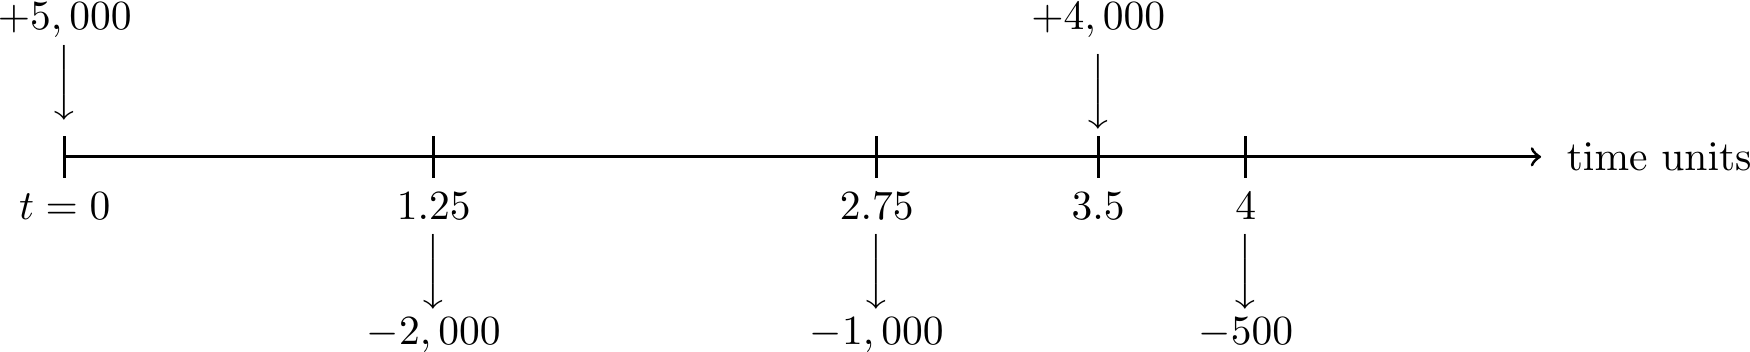
\includegraphics{SCMA266Bookdownproj_files/figure-latex/tikz-exam3-1} \end{center}

\begin{enumerate}
\def\labelenumi{\arabic{enumi}.}
\setcounter{enumi}{4}
\tightlist
\item
  (Excel) It is a good exercise to check whether the Excel worksheet
  you have developed so far for calculating the present value and
  future value can be applied to the questions in this Tutorial. What
  would you do to improve the Excel worksheet for a more general
  scenario?
\end{enumerate}

\section{Tutorial 3}\label{tutorial-3}

\begin{enumerate}
\def\labelenumi{\arabic{enumi}.}
\item
  Calculate the present value now of an annuity payable monthly in
  advance. The annual amount of the annuity will be \$ 2,400 for the
  first 10 years and \$ 3,600 for the next 15 years, after which
  payment will cease. Assume that the effective rate of interest is 2\%
  per annum.
\item
  Assume that the effective rate of interest will be 3\% for 5 years
  from now, 4\% for the next 5 years and 5\% thereafter. Calculate the
  following values:

  \begin{enumerate}
  \def\labelenumii{\arabic{enumii}.}
  \item
    The present value of an annuity of \$ 1,000 per annum, payable
    in arrear for 15 years.
  \item
    The present value of an annuity due of \$ 500 per annum, payable
    at the beginning of the year for 20 years.
  \item
    The accumulation value of an increasing annuity payable yearly
    in arrear for 30 years. The first annual payment is \$ 100, and
    payments will be increase by \$ 100 each year.
  \item
    The accumulation value of an increasing annuity payable yearly
    in advance for 18 years. The first annual payment is \$ 1,000,
    and payments will be increase by 2\% each year (compound).
  \item
    The present value of an annuity of \$ 200, payable in arrear for
    10 years and deferred for 3 years.
  \end{enumerate}
\item
  You borrow \$ 240,000 from a bank to be repaid by the end of 5
  years. Assume that the interest rate is 4\% per annum. Consider the
  following four possible options for the loan to be repaid.

  \begin{enumerate}
  \def\labelenumii{\arabic{enumii}.}
  \item
    Calculate the amount of the repayments to repay if you choose to
    repay the loan as late as possible.
  \item
    You may choose to repay interest only during the 5 years term of
    loan and repay the capital at the end of the term. Calculate
    interest to be repaid and draw the timeline to illustrate the
    cashflows for the repayment of the loan.
  \item
    Calculate the amount X of level instalments to repay the loan
    which will be paid at the end of each year for 5 years and draw
    the timeline to illustrate the cashflows for the repayment of
    the loan.
  \item
    Calculate the amount Y of level instalments to repay the loan
    which will be paid at the end of each month for 5 years and draw
    the timeline to illustrate the cashflows for the repayment of
    the loan. \textbf{Instalment} is a sum of money due as one of several
    equal payments for something, spread over an agreed period of
    time.
  \end{enumerate}
\item
  A person now age 30 has received a pension from a company. When he
  retires at age 60, he will be paid on each birthday from the 60 to
  the 85th inclusive. The first annual payment will be half of his
  salary when he retires, and payments will then increase by 2\%
  compounding each year. Currently, he receive a salary of \$ 20,000
  and will increase by 3\% each year compounding in line with
  inflation. Assume that the effective rate of interest will be 4\% for
  the next 20 years and 5\% thereafter. Calculate the present value now
  of this pension.
\item
  (Excel) Use Excel worksheet you have developed so far to calculate
  the results from the questions in this Tutorial.
\end{enumerate}

\section{Tutorial 4}\label{tutorial-4}

\begin{enumerate}
\def\labelenumi{\arabic{enumi}.}
\item
  Show that the following series of cashflows are equivalent given
  that an interest rate is 4\% per annum effective.

  \begin{enumerate}
  \def\labelenumii{\arabic{enumii}.}
  \item
    One single payment of amount 14,802.44 at year 10.
  \item
    a level annuity of 400 payable yearly in arrear for the next 10
    years plus a lump sum of 10,000.
  \item
    a level annuity of 1,232.91 payable yearly in arrear for the
    next 10 years.
  \end{enumerate}
\item
  You invest in a project which requires you to pay 2,000 and receive
  back 300 at the end of each of the next 8 years. Calculate the yield
  of this investment. ANS = 4.2394551\%
\item
  You pay a price of 5,000 for an investment that will repay you 600
  per annum payable half-yearly in arrear for the next 12 years.
  Calculate the yield of this investment. ANS = 3.1491266\%
\item
  An investor pays 100,000 in order to receive 20,000 back at the end
  of the first 3 years and 25,000 back at the end in the next 4 years.
  Calculate the yield of this investment. ANS = 12.6209232\%
\item
  You invest in a project which requires you to pay 500,000 at the
  start of each of the calendar years 2018, 2019 and 2020. The project
  is expected to return profits of 400,000 for 6 years a the end of
  each calendar year 2024 to 2029 inclusive. Calculate the yield of
  this investment. ANS = 5.7285486\%
\item
  (Modified from CT1 2012 IFoA Exam)

  An investor is considering two projects, Project A and Project B.
  Project A involves the investment of 2,000,000 in a retail outlet.
  Rent is received quarterly in arrear for 25 years, at an initial
  rate of 100,000 per annum. It is assumed that the rent will increase
  at a rate of 5\% per annum compound, but with increases taking place
  every five years. Maintenance and other expenses are incurred
  quarterly in arrear, at a rate of 12,000 per annum. The retail
  outlet reverts to its original owner after 25 years for no payment.

  Project B involves the purchase of an office building for 1,000,000.
  The rent is to be received quarterly in advance at an initial rate
  of 85,000 per annum. It is assumed that the rent will increase to
  90,000 per annum after 20 years. There are no maintenance or other
  expenses. After 25 years the property reverts to its original owner
  for no payment.

  Calculate the annual effective internal rate of return for both
  Projects A and B. Which project is preferable?
\item
  (Excel) Use Excel worksheet you have developed to calculate the
  results from the questions in this Tutorial.
\end{enumerate}

\section{Tutorial 5}\label{tutorial-5}

\begin{enumerate}
\def\labelenumi{\arabic{enumi}.}
\item
  You borrow 30,000 for a term of 6 months to be repaid in arrear by
  level monthly instalments. The rate of interest will be 4\% pa
  effective.

  \begin{enumerate}
  \def\labelenumii{\arabic{enumii}.}
  \item
    Calculate the monthly repayment.
  \item
    Construct the complete loan schedule
  \end{enumerate}
\item
  A loan of 800,000 is repayable by equal monthly repayments for 10
  years, with interest rate payable at 6.5\% pa effective.

  \begin{enumerate}
  \def\labelenumii{\arabic{enumii}.}
  \item
    Calculate the amount of each monthly payment.
  \item
    Calculate the interest and capital contents of the 96th
    repayment.
  \end{enumerate}
\item
  \begin{enumerate}
  \def\labelenumii{\arabic{enumii}.}
  \item
    An investor takes out a loan of 100,000 from a bank to be repaid
    by level annual instalments in arrear over 12 years where the
    bank charges an effective annual rate of interest of 7\%.
    Immediately after the 6th repayment has been made, the investor
    may

    \begin{enumerate}
    \def\labelenumiii{\arabic{enumiii}.}
    \item
      extend the term of the loan by extra 2 year, or
    \item
      miss the next two repayments.
    \end{enumerate}

    Calculate the revised repayment amount in each case.
  \item
    Suppose the bank allows the
    investor to miss the next two repayments but the capital
    outstanding will be charged interest at 10\% pa effective while
    the investor is not making repayments. Calculate the revised
    repayment.
  \item
    Suppose in Question 3.2 that the investor will miss the next two
    repayment and extend the term of the loan by extra 4 years.
    Calculate the revised repayment.
  \end{enumerate}
\item
  An investor borrows 50,000 for a term of 12 years. The rate of
  interest will be 4\% pa effective for the first 6 years and 5\% pa
  effective thereafter. The loan will be repaid level annual
  repayments for the first 6 years, and then increasing to twice the
  origin level for the last 6 years. Calculate the annual repayment.
\item
  An investor borrows 40,000 for a term of 10 years. The rate of
  interest will be 6.5\% pa effective The loan will be repaid level
  annual repayments, increasing at 2\% per annum.

  \begin{enumerate}
  \def\labelenumii{\arabic{enumii}.}
  \item
    Calculate the first annual repayment.
  \item
    Calculate the capital outstanding after the 7th repayment is
    made.
  \item
    Calculate the interest content of the 8th repayment.
  \end{enumerate}
\item
  (Excel) Suppose you borrow \(L\) from a bank to be repaid by the end
  of \(n\) years at an interest rate of \(i\%\) per annum effective. If
  you agree to repay the loan and the interest in equal annual
  instalments throughout term of loan and the first payment is made at
  the end of the first year.

  Create a model to produce a loan amortisation (or loan schedule)
  table. Make the interest rate, loan life, initial loan, and other
  necessary variables input variables. The loan amortisation table
  should include the following columns:

  \begin{itemize}
  \item
    The year-beginning balance
  \item
    The annual repayment
  \item
    Interest Component
  \item
    Capital content
  \item
    Capital outstanding (the year-end balance)
  \end{itemize}
\end{enumerate}

\section{Tutorial 6}\label{tutorial-6}

\begin{enumerate}
\def\labelenumi{\arabic{enumi}.}
\item
  A company issues a bond of nominal amount 10,000 with a term of 5
  years and a coupon of 6\% convertible semiannually, to be redeemed at
  110\%. Calculate the price of the bond to give a redemption yield of
  8\% pa effective to an investor who pays no tax.
\item
  A 10-year bond of nominal amount 1,000 paying a half-yearly coupon of
  10\% per annum and redeemable at par. Calculate the price of this
  bond to give a redemption yield of 7\% per annum effective after
  taxes to

  \begin{enumerate}
  \def\labelenumii{\arabic{enumii}.}
  \item
    an investor who pays no taxes.
  \item
    an investor who is subject to income tax at 15\% but no CGT.
  \item
    an investor who is subject to
    income tax at 15\% and CGT at 20\%.
  \item
    If the investor question 2.3 would like to secure a redemption yield of 9\%
    pa, calculate the price for the bond.
  \end{enumerate}
\item
  An investor who pays income tax at 20\%, but no CGT buys a 15-year
  bond to be redeemed at 105\%, bearing semi-annual coupons of 10\% pa.

  \begin{enumerate}
  \def\labelenumii{\arabic{enumii}.}
  \item
    Calculate the price per 100 THB nominal to give a yield of 9\% pa
    effective.
  \item
    Just after the 20th coupon payment, the income tax rate changes
    to 15\%. If the investor holds the bond to redemption, calculate
    the realised yield on the whole transaction.
  \end{enumerate}
\item
  A 15-bond of a nominal amount of 10,000 THB, bearing semi-annual coupons
  of 6\% pa, to be redeemed at 98\%.

  \begin{enumerate}
  \def\labelenumii{\arabic{enumii}.}
  \item
    An investor who is subject to income tax at 30\% and CGT at 20\%
    buys this bond for 9,000 THB. Calculate the net yield per annum for
    this transaction.
  \item
    If the investor wishes to obtain a net redemption yield of 7\%
    pa, calculate the price that the investor should pay for the
    bond.
  \end{enumerate}
\item
  A company issues a bond of nominal 100 THB amount with a term of 15 years
  and a coupon of 7\% convertible semiannually, to be redeemed at par.

  \begin{enumerate}
  \def\labelenumii{\arabic{enumii}.}
  \item
    Calculate the price of the bond if it is priced at issue to give
    a redemption yield of 8\% pa effective to a non-tax paying
    investor.
  \item
    Investor A liable to income tax at 25\% and capital gain tax at
    20\% bought the bond on the issue date. Just after the 15th
    coupon payment, the investor A sold the bond to Investor B. The
    investor B, subject to income tax at 30\% and capital gain tax at
    30\% paid the price that gives a net redemption yield of 6.5\%.
    Calculate the price that investor B paid.
  \item
    Calculate the realised yield for Investor A's transaction.
  \end{enumerate}
\end{enumerate}

\section{Tutorial 7}\label{tutorial-7}

\begin{enumerate}
\def\labelenumi{\arabic{enumi}.}
\item
  Consider a 5-year bond of a nominal amount of 100 THB , bearing annual
  coupons of 8\% pa, to be redeemed at 110\%. The bond was issued in
  July 2012 and its issue price was 100\%. With reference to the CPI
  given in the lecture note, show that the real yield to an investor
  who is not subject to tax is 8.82\%.
\item
  A particular transaction will provide an effective rate of interest
  of 6\% per annum. The period of the transaction is one year.

  \begin{enumerate}
  \def\labelenumii{\arabic{enumii}.}
  \item
    If the annual inflation rate over this one year period will be
    constant and equal to 2.5\%, calculate the real yield on this
    transaction.
  \item
    Calculate the constant annual rate of inflation at which the
    investor will obtain a real yield on this transaction of at
    least 4.25\% per annum.
  \item
    Calculate the real yield on this transaction if inflation will
    be 3\% pa for the first nine months of the year and then 3.25\%pa
    for the remaining three months.
  \end{enumerate}
\item
  Consider a 3-year bond of a nominal amount of 100 THB, bearing annual
  coupons of 6\% pa, to be redeemed at par. The bond was issued in 15
  January 2015 and its issue price was 95\%.

  An investor who pays no tax purchased this bond on the issue date
  and held it until redemption.

  \begin{enumerate}
  \def\labelenumii{\arabic{enumii}.}
  \item
    Show that the yield obtained by this investor is approximately
    7.94\%.
  \item
    Show that the real yield on this investment is approximately
    1.80\% assuming the CPI values are given below:

    \begin{longtable}[]{@{}rrrrr@{}}
    \toprule\noalign{}
    Year & 2015 & 2016 & 2017 & 2018 \\
    \midrule\noalign{}
    \endhead
    \bottomrule\noalign{}
    \endlastfoot
    CPI on 15 January & 100 & 103.3 & 111.0 & 119.5 \\
    \end{longtable}
  \end{enumerate}
\item
  An investor who is not liable to tax had the choice of purchasing
  two investments made on 1 Apr 2018.

  \begin{enumerate}
  \def\labelenumii{(\Alph{enumii})}
  \item
    A 10-year bond of a nominal of 100 THB, bearing a half-yearly coupon of
    9\% per annum and redeemable at par. The issue price was at 110\%.
  \item
    A 10-year index linked bond at a price of 135 THB per 100 THB nominal, bearing a
    half-yearly coupon of 4\% per annum and redeemable at par. The
    CPI base figure for indexing is 100.24 and the CPI figure
    applicable to the next coupon (payable on 1 Oct 2018) is 145.68.
    (Here 145.68 is the CPI index on 1 Apr 2018).
  \end{enumerate}

  Assume that CPI will grow at a rate of 2.5\% per annum from its
  latest known value of 145.68 on 1 Apr 2018.

  \begin{enumerate}
  \def\labelenumii{\arabic{enumii}.}
  \item
    Calculate the real rate of return (yield) per annum earned on
    both investments A and B.
  \item
    Determine which of the two investments yielded the highest real
    rate of return per annum.
  \end{enumerate}
\item
  An investor who is not liable to tax had the choice of purchasing
  two investments made on 15 Jan 2013.

  \begin{enumerate}
  \def\labelenumii{(\Alph{enumii})}
  \item
    50,000 was placed in a 5-year term special saving account. The
    effective rate of interest was 2.5\% p.a. for the first year, 3.5
    \% p.a. for the second year, 4.5 \% p.a. for the third year, 5.5\%
    p.a. for the fourth year and 6.5\% p.a. for the fifth year.
  \item
    50,000 was used to purchase an annuity payable annually in arrears
    for 5 years to yield 6\% p.a. effective.
  \end{enumerate}

  Assume that the values of CPI are as follows:

  \begin{longtable}[]{@{}rrrrrrr@{}}
  \toprule\noalign{}
  Year & 2013 & 2014 & 2015 & 2016 & 2017 & 2018 \\
  \midrule\noalign{}
  \endhead
  \bottomrule\noalign{}
  \endlastfoot
  CPI on 15 January & 100 & 104.17 & 110.17 & 111.08 & 112.67 & 114.83 \\
  \end{longtable}

  \begin{enumerate}
  \def\labelenumii{\arabic{enumii}.}
  \item
    Calculate the real rate of return (yield) per annum earned on
    both investments A and B.
  \item
    Determine which of the two investments yielded the highest real
    rate of return per annum.
  \end{enumerate}
\end{enumerate}

\section{Tutorial 8}\label{tutorial-8}

\begin{enumerate}
\def\labelenumi{\arabic{enumi}.}
\item
  10,000 was placed in a 3-year term special saving account on 15
  Jan 2015. The effective rate of interest was 2.5\% p.a. for the first
  year, 3.5 \% p.a. for the second year, 4.5 \% p.a. for the third year.
  Assume that the values of CPI are as follows:

  \begin{longtable}[]{@{}rrrrrll@{}}
  \toprule\noalign{}
  Year & 2015 & 2016 & 2017 & 2018 & & \\
  \midrule\noalign{}
  \endhead
  \bottomrule\noalign{}
  \endlastfoot
  CPI on 15 January & 100 & 104.08 & 106.67 & 108.83 & & \\
  \end{longtable}

  What is the real rate of return (yield) per annum earned on this
  investment?

  \begin{enumerate}
  \def\labelenumii{\Alph{enumii}.}
  \item
    0.618\%
  \item
    0.629\%
  \item
    0.724\%
  \item
    0.762\%
  \item
    none of the above
  \end{enumerate}
\item
  A company's cash position, measured in
  million of bahts, follows a generalised Wiener process with a drift
  rate of 0.25 per quarter and a variance rate of 9 per quarter. The
  initial cash position is 35. What is the expected cash position at
  the end of 6 months?

  \begin{enumerate}
  \def\labelenumii{\Alph{enumii}.}
  \item
    35.25
  \item
    35.5
  \item
    35.75
  \item
    36
  \item
    none of the above
  \end{enumerate}
\item
  Suppose that data on a stock price at
  the end of 63 consecutive trading days gives the sum of the daily
  returns \[\sum_{i=1}^{62} \ln(S_i/S_{i-1}) = 0.25\] and the sum of
  the daily returns squared
  \[\sum_{i=1}^{62} \left( \ln(S_i/S_{i-1}) \right)^2= 0.0042.\]
  Assume that there are 252 trading days per year. What is the
  estimated value of the stock price volatility per annum?

  \begin{enumerate}
  \def\labelenumii{\Alph{enumii}.}
  \item
    9.28\%
  \item
    10.72\%
  \item
    11.42\%
  \item
    12.37\%
  \item
    none of the above
  \end{enumerate}
\item
  What is the standard error (per annum) of the estimate obtained in Question 3?

  \begin{enumerate}
  \def\labelenumii{\Alph{enumii}.}
  \item
    0.72\%
  \item
    0.85\%
  \item
    0.93\%
  \item
    1.02\%
  \item
    none of the above
  \end{enumerate}
\item
  With the drift rate and the variance rate as given in the Question 2, What is the
  company's initial cash position so that the company has a less than
  5\% chance of a negative cash position by the end of 1 year? Note
  that \(\Pr( Z \le 1.645) = 0.95\) for a standard normal random number
  \(Z\).

  \begin{enumerate}
  \def\labelenumii{\Alph{enumii}.}
  \item
    6.48
  \item
    6.84
  \item
    7.29
  \item
    7.92
  \item
    none of the above
  \end{enumerate}
\item
  Suppose that a stock price follow geometric Brownian motion with an
  initial price of 40 TBH, an expected return of 8\% per annum and a
  volatility of 30\% per annum. Using monthly time steps and the random
  samples from a normal distribution given in the table below, what is
  the simulated value of the stock price path at time 3 months?

  \begin{longtable}[]{@{}lrrrlll@{}}
  \toprule\noalign{}
  Period (n) & 1 & 2 & 3 & & & \\
  \midrule\noalign{}
  \endhead
  \bottomrule\noalign{}
  \endlastfoot
  Random sample from \(N(0,1)\) for period \(n\) & 0.62 & 1.34 & -0.76 & & & \\
  \end{longtable}

  \begin{enumerate}
  \def\labelenumii{\Alph{enumii}.}
  \item
    45.92
  \item
    46.78
  \item
    47.40
  \item
    48.80
  \item
    none of the above
  \end{enumerate}
\item
  An investor who was not subject to tax purchased an index-linked
  bond issued on 15 January 2016 with a term of 2 years. The annual
  coupon rate was 2\% p.a. payable half-yearly in arrears and the
  redemption rate was 100\%. The coupons and redemption payments were
  adjusted with reference to the CPI value of 3 months before the
  payments were made.

  The value of the inflation index at particular dates are as follows:

  \begin{longtable}[]{@{}lrrrrrrrrrr@{}}
  \toprule\noalign{}
  Date & Oct 15 & Jan 16 & Apr 16 & Jul 16 & Oct 16 & Jan 17 & Apr 17 & Jul 17 & Oct 17 & Jan 18 \\
  \midrule\noalign{}
  \endhead
  \bottomrule\noalign{}
  \endlastfoot
  CPI (Date) & 96 & 97 & 99 & 100 & 102 & 104 & 105 & 109 & 111 & 112 \\
  \end{longtable}

  \begin{enumerate}
  \def\labelenumii{\arabic{enumii}.}
  \item
    Write down the value of the base CPI figure.
  \item
    Calculate the actual payments per 100 THB nominal received by
    the investor. Clearly state the date on which each payment was
    received.
  \item
    Calculate the real payments per 100 THB nominal in terms of
    their purchasing power at 15 January 2016.
  \item
    Calculate the purchase price of the bond per 100 THB nominal if
    the investor obtained a \ul{\textbf{real}} redemption yield of
    0.79\% p.a. effective on the bond.
  \end{enumerate}
\item
  Consider a stock that pays no dividends, provides an expected return
  of 10\% per annum with continuous compounding and has a volatility of
  25\% per annum. Assume that the stock price follows geometric
  Brownian motion and its current stock price is 40 THB.

  \begin{enumerate}
  \def\labelenumii{\arabic{enumii}.}
  \item
    Find the probability distribution of the logarithm of the stock
    price \(S_T\) in 6 months' time.
  \item
    Calculate the mean and the standard deviation of \(\ln S_T\) in 6
    months' time.
  \item
    Find the 95\% confidence interval of \(S_T\) in 6 months' time.
  \end{enumerate}
\end{enumerate}

\chapter{Solutions to Tutorials}\label{solutions-to-tutorials}

\section{Solutions to Tutorial 1}\label{solutions-to-tutorial-1}

\begin{enumerate}
\def\labelenumi{\arabic{enumi}.}
\item
  The solutions to each question are as follows:

  \begin{enumerate}
  \def\labelenumii{\arabic{enumii}.}
  \tightlist
  \item
    \(5000 (1.075)^4 = 6677.345703\)
  \item
    Let \(i\%\) be the annual rate effective equivalent to \(3\%\) per quarter-effective, \(i = (1.03)^4 - 1\).
    Hence, the accumulation is
    \[800(1+i)^{2.7} = 800(1.03)^{4\times2.7} = 1100.859802.\]
  \item
    Let \(j\%\) be the monthly rate effective equivalent to \(4.25\%\) per half-year effective, \(j = (1.0425)^{2/12} - 1\).
    Hence, the accumulation is
    \[10000(1.0425)^{(2/12)\times27} = 12059.86056.\]
  \end{enumerate}
\item
  The solutions to each question are as follows:

  \begin{enumerate}
  \def\labelenumii{\arabic{enumii}.}
  \tightlist
  \item
    \(\frac{1000}{1.075} = 930.232558\).
  \item
    \(\frac{100}{(1.03)^7} = 81.309151\).
  \item
    Let \(j\%\) be the quarterly rate effective equivalent to \(4.25\%\) per half-year effective, \(j = (1.0425)^{2/4} - 1\).
    Hence, the present value is
    \[10000\times (1+j)^{-5} = 10000(1.0425)^{-(5/2)} = 9011.764643.\]
  \end{enumerate}
\item
  The solutions to each question are as follows:

  \begin{enumerate}
  \def\labelenumii{\arabic{enumii}.}
  \tightlist
  \item
    0.3274\%
  \item
    3.1988\%
  \end{enumerate}
\item
  The solutions to each question are as follows:

  \begin{enumerate}
  \def\labelenumii{\arabic{enumii}.}
  \tightlist
  \item
    500(1.04)(1.05)(1.06) =578.76
  \item
    \(2000(1.04)^{3/4}(1.05)(1.06)^{3/4} =2259.299\)
  \item
    (1.04)(1.05)(1.06) = 1.15752
  \end{enumerate}
\item
  The account balance in 3 years is \(3000(1.025)^{3} = 3230.67\).
\item
  The amount to be repaid for the loan is 5000(1.1) = 5500.
\item
  Let \(X\) be the amount to be deposited now.
  \[X = \frac{1000}{(1.0575)^4} + \frac{2000}{(1.0575)^8} = 2078.36. \]
\item
  At time 3.75 years, Katy has a balance of \(100(1+i)^{15}\). The interest on this balance over the next 3 months is \(100(1+i)^{15}\cdot i\).
  Taylor earns simple interest on the original amount which is equal to \(500i\cdot\frac{3}{12}\). Therefore, we solve for \(i\) from the following equation:
  \[ 100(1+i)^{15}\cdot i = 500i\cdot\frac{3}{12},\] which gives \(i = 0.014987.\)
\item
  The timeline for the following annuity having cashflow of 1 unit at the end of each of the next \(n\) time units is given in the figure below:
\end{enumerate}

\begin{center}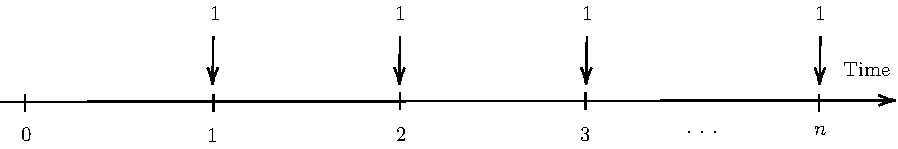
\includegraphics{SCMA266Bookdownproj_files/figure-latex/tikz-sol1-1} \end{center}

\begin{enumerate}
\def\labelenumi{\arabic{enumi}.}
\setcounter{enumi}{9}
\tightlist
\item
  (More details in the course ``Life Contingencies I''). We need to define a random variable \(T_x\) = the remaining future life time of a life aged \(x\).
\end{enumerate}

\begin{center}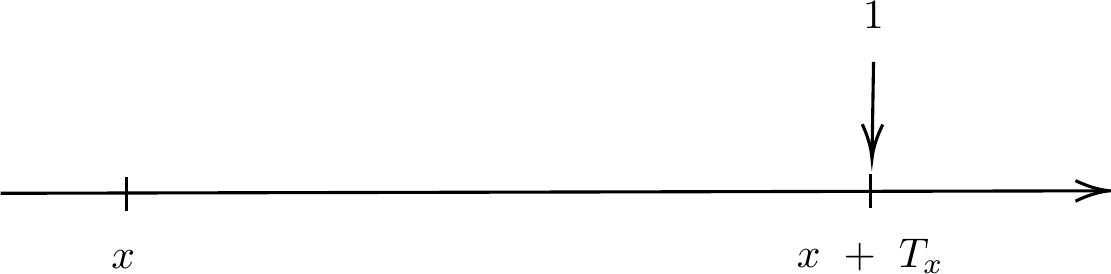
\includegraphics{SCMA266Bookdownproj_files/figure-latex/tikz-sol2-1} \end{center}

The quantity of interest is the present value of the death benefit assuming the interest rate of \(i\%\) p.a. effective. It is also a random variable,
\[PV = \frac{1}{(1+i)^{T_x}}.\] It turns out that the premium rate of this whole life insurance is \(E[PV]\), the expected value of the present value, \(PV\).

\section{Solutions to Tutorial 2}\label{solutions-to-tutorial-2}

\begin{enumerate}
\def\labelenumi{\arabic{enumi}.}
\item
  The solutions to each question are as follows:

  \begin{enumerate}
  \def\labelenumii{\arabic{enumii}.}
  \tightlist
  \item
    \((1.03)^3(1.04)^{2.5} (1.02)^{12} = 1.528611\)
  \item
    \(5000A(0.5,2.75) = 5000(1.03)(1.04)^{2.5} (1.02)^{9} = 6788.786068\)
  \item
    We first find the rate \(j\%\) per month effective that is equivalent to the rate of \(4\%\) per half-year effective.
    \[j = (1.04)^{1/6} - 1 = 0.00656.\]
    The accumulated value is \(100A(1+2/12, 3 + 7/12 ) = 100(1+j)^{10}(1.02)^{19} = 155.522118.\)
  \item
    \(25000V(0,1.5) = \frac{25000}{(1.03)^3(1.04)^{1.5}} = 21571.39968.\)
  \item
    \(8000V(0.25,2.75) = \frac{8000}{(1.03)^2(1.04)^{2.5}(1.02)^{9}} = 5720.455921.\)
  \item
    \(V(0.5,1.75) = \frac{1}{(1.03)(1.04)^{2}} = 0.897627.\)
  \end{enumerate}
\item
  The solutions to each question are as follows:

  \begin{enumerate}
  \def\labelenumii{\arabic{enumii}.}
  \tightlist
  \item
    With \(i = 7.25\%\) per time period, \(V(4) = 100 (1+i)^4 - 30(1+i)^3 - 30 (1+i)^2 + 100 (1+i) - 30 = 138.041762.\)
  \item
    \(V(8) = V(4)\cdot (1+i)^4 = 182.641597.\)
  \item
    \(PV(0) = V(4)\cdot (1+i)^{-4} = 104.332903.\)
  \end{enumerate}
\item
  The solutions to each question are as follows:

  \begin{enumerate}
  \def\labelenumii{\arabic{enumii}.}
  \tightlist
  \item
    With \$ = 6\%\$ per time period, \(V(5) = 5000 (1+i)^5 - 2000(1+i)^{3.75} - 1000 (1+i)^{2.25} + 4000 (1+i)^{1.5} - 500(1+i) = 6897.948585.\)
  \item
    \(V(2) = V(5)(1+i)^{-3} = 5791.650645.\)
  \item
    \(PV(0) = V(5)(1+i)^{-5} = 5154.548456.\)
  \end{enumerate}
\item
  The solutions to each question are as follows:

  \begin{enumerate}
  \def\labelenumii{\arabic{enumii}.}
  \tightlist
  \item
    \(V(1/1/2019) = 100(1.04)(1.03)^{3.5}(1.015)^{15} - 30 (1.03)^{3.5}     (1.015)^{15}- 30 (1.03)^{1.5} (1.015)^{15} + 100 (1.015)^{12} - 30 = 152.955693.\)
  \item
    \(PV(0)= V(1/1/2015) = \frac{152.955693}{(1.04)(1.03)^{3.5}(1.015)^{15}} =106.074596.\)
  \item
    \(V(1/7/2017) = PV(0)(1.04)(1.03)^3 = 120.546998.\)
  \end{enumerate}
\end{enumerate}

\section{Solutions to Tutorial 3}\label{solutions-to-tutorial-3}

\begin{enumerate}
\def\labelenumi{\arabic{enumi}.}
\tightlist
\item
  Let \(j\) be the effective rate per month equivalent to \(i = 2\)\%. We have
  \[ j = (1.02)^{1/12}  - 1= 0.001652. \]
  Hence,
\end{enumerate}

\[ PV(0) = 200 \ddot{a}^{j}_{120} + 300 \ddot{a}^{j}_{180} \left( \frac{1}{1.02} \right)^{10} = 60148.03. \]

\begin{enumerate}
\def\labelenumi{\arabic{enumi}.}
\setcounter{enumi}{1}
\item
  The solutions to each question are as follows:

  \begin{enumerate}
  \def\labelenumii{\arabic{enumii}.}
  \item
    The cashflows have been splitted into three periods: (a) from time point 0-5, (b) 5-10 and (c) time point 10 onward.
    \[PV(0) = 1000 ( a^{3\%}_{5} + 1.03^{-5} a^{4\%}_{5} +  1.03^{-5} 1.04^{-5} a^{5\%}_{5}) = 11489.49  \]
  \item
    We have
    \[PV(0) = 500 ( \ddot{a}^{3\%}_{5} + 1.03^{-5} \ddot{a}^{4\%}_{5} +  1.03^{-5} 1.04^{-5} \ddot{a}^{5\%}_{10}) = 7229.67  \]
  \item
    The accumuated value is
    \[100 (Is)^{3\%}_{5} (1.04)^5 (1.05)^{20} + \left[100 (Is)^{4\%}_{5} + 500 s^{4\%}_{5} \right] (1.05)^{20}  + \left[100 (Is)^{5\%}_{20} + 1000 s^{5\%}_{20} \right]= 78929.01  \]
  \item
    Let \(i_1 = 3\%, i_2 = 4\%\) and \(i_3 = 5\%\). The accumuated value is given by
    \[\begin{aligned} 
     V(18) &= \left[1000(1+i_1)^5 + 1000(1.02)(1+i_1)^4 + 1000(1.02)^2(1+i_1)^3 + \ldots + 1000(1.02)^4(1+i_1)\right](1.04)^5(1.05)^8   \\
     &+ \left[1000(1.02)^5(1+i_2)^5 + 1000(1.02)^6(1+i_2)^4 + 1000(1.02)^7(1+i_2)^3 + \ldots + 1000(1.02)^9(1+i_2)\right](1.05)^8   \\
     &+ \left[1000(1.02)^{10}(1+i_3)^8 + 1000(1.02)^{11}(1+i_3)^7 + 1000(1.02)^{12}(1+i_3)^6 + \ldots + 1000(1.02)^{17}(1+i_3)\right]  \\
     &= 1000(1.02)^5 \left[ \left(\frac{1+i_1}{1.02}\right)^5   + \left(\frac{1+i_1}{1.02}\right)^4 + \ldots + \left(\frac{1+i_1}{1.02}\right) \right](1.04)^5(1.05)^8 \\
     &+ 1000(1.02)^{10} \left[ \left(\frac{1+i_2}{1.02}\right)^5   + \left(\frac{1+i_2}{1.02}\right)^4 + \ldots + \left(\frac{1+i_2}{1.02}\right) \right](1.05)^8 \\
      &+ 1000(1.02)^{18} \left[ \left(\frac{1+i_3}{1.02}\right)^8   + \left(\frac{1+i_3}{1.02}\right)^7 + \ldots + \left(\frac{1+i_3}{1.02}\right) \right] 
     \end{aligned}\]
    Let \(1+j_1  = \frac{1+i_1}{1.02}\). Then, \(j_1 = 0.009804\) and
    \[ \left[ \left(\frac{1+i_1}{1.02}\right)^5   + \left(\frac{1+i_1}{1.02}\right)^4 + \ldots + \left(\frac{1+i_1}{1.02}\right) \right] = \frac{(1+j_1)^5 - 1}{j_1/(1+j_1)} = 5.148995.\]
    Let \(1+j_2  = \frac{1+i_2}{1.02}\). Then, \(j_2 = 0.019608\) and
    \[ \left[ \left(\frac{1+i_2}{1.02}\right)^5   + \left(\frac{1+i_2}{1.02}\right)^4 + \ldots + \left(\frac{1+i_2}{1.02}\right) \right] = 5.301921.\]
    Let \(1+j_3  = \frac{1+i_3}{1.02}\). Then, \(j_3 = 0.029412\) and
    \[ \left[ \left(\frac{1+i_3}{1.02}\right)^8   + \left(\frac{1+i_3}{1.02}\right)^7 + \ldots + \left(\frac{1+i_3}{1.02}\right) \right]  = 9.134790.\]
    Therefore, \(V(18) = 32814.45\).
  \item
    The present value is
  \end{enumerate}
\end{enumerate}

\[\begin{aligned}
    PV(0) &= \left( \frac{200}{(1.03)^4} + \frac{200}{(1.03)^5}\right) + 200 a^{0.04}_5 (1.03)^{-5} + 200 a^{0.05}_{3} (1.03)^{-5} (1.04)^{-5} \\
    &= 350.2192 + 768.0362 + 386.1574 = 1504.413
\end{aligned}\]

\begin{enumerate}
\def\labelenumi{\arabic{enumi}.}
\setcounter{enumi}{2}
\item
  The solutions to each question are as follows:

  \begin{enumerate}
  \def\labelenumii{\arabic{enumii}.}
  \tightlist
  \item
    \(240000 (1.04)^5 = 291996.7\)
  \item
    The interest amounts are \(0.04\times 240000 = 9600.\)
  \item
    By the Principle of Equivalence, we have
    \[ 240000 = X a^{0.04}_{5}. \]
    This gives X = 53910.51.
  \item
    Level installments are payable monthly, which follows
    \[ 240000 = Y a^{j}_{60}, \]
    where \(j = (1.04)^{1/12} - 1\). This gives Y = 4412.23.
  \end{enumerate}
\item
  The person retires in 30 years, when his salary is expected to be
  \(20000 \times (1.03)^{30} = 48545.25.\)
  The first payment will be half of this which is equal to 24272.62.
  The present value at age 60 of his pension is
  \[  24272.62 \times \ddot{a}^{0.029412}_{26} = 449717.9\] (the precise value is 449719.051954).
  Here we use \(\frac{1.05}{1.02} = 1.029412\) and the annuity is paid from the 60th to the 85th birthday inclusive so there are 26 payments made in advance.
  Therefore, the present value of this at age 30 is
  \[ 449717.9 \times (1.05)^{-10} \times (1.04)^{-20} = 126002.9. \]
  (the precise value is 126003.181173)
\end{enumerate}

\section{Solutions to Tutorial 4}\label{solutions-to-tutorial-4}

\begin{enumerate}
\def\labelenumi{\arabic{enumi}.}
\item
  To examine whether the cashflows are equivalent, we compare their present values.

  \begin{enumerate}
  \def\labelenumii{\alph{enumii}.}
  \item
    The present value of single payment of amount 14,802.44 at year 10 is
    \[ PV(0) =  \frac{14,802.44}{1.04^{10}} = 10000.\]
  \item
    The present value of the level annuity of 400 payable yearly in arrears for the next 10 years plus a lump sum of 10,000 is
    \[ PV(0) =  400 a^{0.04}_{10} +\frac{10000}{1.04^{10}} = 10000.\]
  \item
    The present value of the level annuity of 1,232.91 payable yearly in arrears for the next 10 years.
    \[ PV(0) =  1,232.91 a^{0.04}_{10}  = 10000.\]
  \end{enumerate}
\end{enumerate}

It follows that the values of these cashflows are the same, i.e.~equivalent.

\begin{enumerate}
\def\labelenumi{\arabic{enumi}.}
\setcounter{enumi}{1}
\item
  The annual yield of this investment \(i\) is the solution of the equation of value:
  \[ f(i) = -2000(1+i)^8 +300 s^i_8 = 0. \]
  If we solve using software, we get \(i = 4.2394551%
  \). Instead of using software, you can also use linear interpolation to approximate the solution.
\item
  Working in time unit of half year, the equation of value is
  \[ f(i) = -5000(1+i)^{12 \times 2} + 300 s^i_{24} = 0. \]
  The yield \(i\) per half year is \(i = 3.1491266\%\) and hence the annual yield is \(6.397423\%.\)
\item
  The equation of value is
  \[ f(i) = -100(1+i)^{7} + 20 s^i_{3}(1+i)^{4}  + 25 s^i_{4} = 0. \]
  The annual yield is \(12.6209232\%.\)
\item
  You are suggested to draw the time line for these cashflows. The equation of value is
  \[ f(i) = -5 \ddot{s}^i_{3}(1+i)^{9}   + 4 s^i_{6} = 0. \]
  The annual yield is \(5.7285486\%.\)
\end{enumerate}

\section{Solutions to Tutorial 5}\label{solutions-to-tutorial-5}

\begin{enumerate}
\def\labelenumi{\arabic{enumi}.}
\tightlist
\item
  The monthly repayment can be calculated from this equation
  \[ X = \frac{30000}{a^j_6} = \frac{30000}{5.931847} = 5057.45,\]
  where \(j = (1.04)^{1/12} - 1 = 0.003274.\)
\end{enumerate}

The complete loan schedule is illustrated below:

\begin{longtable}[]{@{}
  >{\centering\arraybackslash}p{(\columnwidth - 8\tabcolsep) * \real{0.2000}}
  >{\centering\arraybackslash}p{(\columnwidth - 8\tabcolsep) * \real{0.2000}}
  >{\centering\arraybackslash}p{(\columnwidth - 8\tabcolsep) * \real{0.2000}}
  >{\centering\arraybackslash}p{(\columnwidth - 8\tabcolsep) * \real{0.2000}}
  >{\centering\arraybackslash}p{(\columnwidth - 8\tabcolsep) * \real{0.2000}}@{}}
\toprule\noalign{}
\begin{minipage}[b]{\linewidth}\centering
Time
\end{minipage} & \begin{minipage}[b]{\linewidth}\centering
Repayment
\end{minipage} & \begin{minipage}[b]{\linewidth}\centering
Interest Content
\end{minipage} & \begin{minipage}[b]{\linewidth}\centering
Capital Content
\end{minipage} & \begin{minipage}[b]{\linewidth}\centering
Capital Outstanding
\end{minipage} \\
\midrule\noalign{}
\endhead
\bottomrule\noalign{}
\endlastfoot
0 & - & - & - & 30000 \\
1 & \(X\) & 98.21 & 4959.23 & 25040.77 \\
2 & \(X\) & 81.98 & 4975.47 & 20065.30 \\
3 & \(X\) & 65.69 & 4991.76 & 15073.54 \\
4 & \(X\) & 49.35 & 5008.10 & 10065.44 \\
5 & \(X\) & 32.95 & 5024.50 & 5040.94 \\
6 & \(X\) & 16.50 & 5040.94 & 0 \\
\end{longtable}

\begin{enumerate}
\def\labelenumi{\arabic{enumi}.}
\setcounter{enumi}{1}
\tightlist
\item
  The monthly repayment can be calculated from this equation
  \[ X = \frac{800000}{a^j_{120}} = \frac{800000}{88.806749} = 9008.32,\]
  where \(j = (1.065)^{1/12} - 1 = 0.005262.\)
\end{enumerate}

The capital outstanding after 95th repayment (25 payments left) is
\[ L_{95} = 9008.32 a^j_{25} = 210506.84.  \]

Hence, the interest content of the 96th repayment is
\[ j \times L_{95} = 0.005262 \times 210506.84 = 1107.62.\]
The capital content of the 96th repayment is
\[ X - 1107.62 = 7900.70. \]

\begin{enumerate}
\def\labelenumi{\arabic{enumi}.}
\setcounter{enumi}{2}
\item
  \begin{enumerate}
  \def\labelenumii{\arabic{enumii}.}
  \tightlist
  \item
  \end{enumerate}

  \begin{enumerate}
  \def\labelenumii{\alph{enumii}.}
  \item
    \textbf{Extending the term of the loan by extra 2 year:} The original repayment is
    \[ X = \frac{100000}{a^{0.07}_{12}} = \frac{100000}{7.942686} = 12590.20,\]
    The capital outstanding after 6th repayment (6 payments left) is
    \[ L_{6} = X a^{0.07}_{6} = 60011.68.  \]
    By extending the term of the loan by extra 2 year, the revised repayment \(X'\) can be obtained (for 8 payments) from
    \[ X' = \frac{L_6}{a^{0.07}_{8}} = 10050.02\]
  \item
    \textbf{Missing the next two repayments:} From the previous result, the capital outstanding after 6th repayment \(L_6 = 60011.68\). Then in 2 years, with interest at \(7\%\) per annum, this accumulates to
    \[ L_6 \times (1.07)^2 = 68707.37. \]
    This must now be repaind by only 4 annual repayments, so the new repayment \(X''\) can be obtained from
    \[ X'' = \frac{68707.37}{a^{0.07}_{4}} = 20284.35.\]
  \end{enumerate}

  \begin{enumerate}
  \def\labelenumii{\arabic{enumii}.}
  \setcounter{enumii}{1}
  \tightlist
  \item
    The capital outstanding will accumulate (at \(10\%\)) to
    \[ L_6 \times (1.1)^2 = 72614.14. \]
  \end{enumerate}

  The new repayment amount \(X'''\) is
  \[X''' = \frac{72614.14}{a^{0.07}_{4}} = 21437.73.\]

  \begin{enumerate}
  \def\labelenumii{\arabic{enumii}.}
  \setcounter{enumii}{2}
  \tightlist
  \item
    The new repayment amount will be
    \[\frac{72614.14}{a^{0.07}_{8}} = 12160.53.\]
  \end{enumerate}
\item
  You are suggested to draw the time line for these cashflows. Let \(X\) be the level of repayment of the first 6 years (\(2X\) will be repaid after this period for the last 6 years). It can be obtained from
  \[ 50000 = X(a^{0.04}_6 + 2 a^{0.05}_6 (1.04)^{-6}) = 3769.34.\]
\item
  \begin{enumerate}
  \def\labelenumii{\arabic{enumii}.}
  \tightlist
  \item
    Let \(X\) be the first annual repayment. Then,\\
    \[ 40000 = X(v + v^2(1.02) + v^3(1.02)^2 + \ldots + v^{10}(1.02)^9),\]
    where \(v = 1/(1.065).\) By rewriting the above equation, we have
    \[ 40000 = \frac{X}{1.02}(\frac{1.02}{1.065} + \left( \frac{1.02}{1.065} \right)^2 + \left( \frac{1.02}{1.065} \right)^3 + \ldots + \left( \frac{1.02}{1.065} \right)^{10}),\]
  \end{enumerate}

  Let \(i' =  \left( \frac{1.065}{1.02} -1 \right) = 0.044118.\) Hence,
  \[ 40000 = \frac{X}{1.02} \cdot a^{i'}_{10},\]
  and \(X = 5133.91.\)

  \begin{enumerate}
  \def\labelenumii{\arabic{enumii}.}
  \setcounter{enumii}{1}
  \tightlist
  \item
    We will calculate the capital outstanding after 7th repayment, \(L_7\) (3 payments left). We first find the amount \(X_8\)of the 8th repayment,
    \[X_8 = X(1.02)^7 = 5897.25.\]
  \end{enumerate}

  So the capital outstanding after the 7th repayment is equal to the present value of the remaining 3 repayments (see the table below).
\end{enumerate}

\begin{longtable}[]{@{}ccccc@{}}
\toprule\noalign{}
Time & 7 & 8 & 9 & 10 \\
\midrule\noalign{}
\endhead
\bottomrule\noalign{}
\endlastfoot
Payment & \(L_7 = ?\) & \(X_8\) & \(X_8 (1.02)\) & \(X_8(1.02)^2\) \\
\end{longtable}

It follows that
\[
\begin{aligned} L_7 &= X_8( v + v^2 + v^3) \\
&= \frac{X_8}{(1.02)} a^{i'}_3 \\
&= 15919.94,
\end{aligned}\]
where \(v\) and \(i'\) are the same as above.

\begin{enumerate}
\def\labelenumi{\arabic{enumi}.}
\setcounter{enumi}{2}
\tightlist
\item
  The interest content of the 8th repayment is
  \[ L_7 * i = 15919.94 \times 0.065 = 1034.80.\]
\end{enumerate}

\section{Solutions to Tutorial 6}\label{solutions-to-tutorial-6}

\begin{enumerate}
\def\labelenumi{\arabic{enumi}.}
\tightlist
\item
  Using a time unit of half a year, the effective yield per half year is
  \[j = (1.08)^{1/2} - 1 = 0.0392305.\]
  Then,
\end{enumerate}

\[
\begin{aligned}
P &= 300 a^j_{\angl{10}} + 11000 (\frac{1}{1.08})^{5} \\
&= 9929.03.
\end{aligned}
\]

\begin{enumerate}
\def\labelenumi{\arabic{enumi}.}
\setcounter{enumi}{1}
\item
  Using a time unit of half a year, the effect yield per half year is
  \[j = (1.07)^{1/2} - 1 = 0.034408.\]

  \begin{enumerate}
  \def\labelenumii{\arabic{enumii}.}
  \tightlist
  \item
    Per 1000 nominal,
    \[
    \begin{aligned}
    P &= 50 a^j_{\angl{20}} + 1000 (\frac{1}{1.07})^{10} \\
    &= 1222.79.
    \end{aligned}
    \]
  \item
    With an income tax rate at 15\%,
  \end{enumerate}
\end{enumerate}

\[
\begin{aligned}
P &= 42.5 a^j_{\angl{20}} + 1000 (\frac{1}{1.07})^{10} \\
&= 1115.62.
\end{aligned}
\]

\begin{verbatim}
3. Since 
\end{verbatim}

\(i^{(2)} = 2 \times j = 0.0688161 < (1 - t_1)\frac{D}{R} = (1 - 0.15)\frac{0.1}{1} = 0.085.\)
Therefore, no capital gain tax (CGT) is payable.
\[
\begin{aligned}
P &= 42.5 a^j_{\angl{20}} + 1000 (\frac{1}{1.07})^{10} \\
&= 1115.62,
\end{aligned}
\]
which is similar to the previous result.

\begin{verbatim}
4. A redepmtion yield of 
\end{verbatim}

9\% p.a. is equivalent to a yield of
\[k = (1.09)^{1/2} - 1 = 0.0440307.\]
Since \(k^{(2)} = 2 \times k = 0.0880613 < (1 - t_1)\frac{D}{R} = (1 - 0.15)\frac{0.1}{1} = 0.085.\)
Therefore, no capital gain tax (CGT) is payable.
\[
\begin{aligned}
P &= 42.5 a^k_{\angl{20}} + (1000 - 0.2(1000-P)) (\frac{1}{1.09})^{10} \\
P &= 978.07 (< 1000).,
\end{aligned}
\]

\begin{enumerate}
\def\labelenumi{\arabic{enumi}.}
\setcounter{enumi}{2}
\item
  The solutions are given below:
\item
  Using a time unit of half a year, the effect yield per half year is
  \[j = (1.09)^{1/2} - 1 = 0.0440307.\]
  Then,
\end{enumerate}

\[
\begin{aligned}
P &= 4 a^j_{\angl{30}} + 105 (\frac{1}{1.09})^{15} \\
&= 94.73.
\end{aligned}
\]
2. In unit of half-year, the timeline of the transaction is shown in the table below:

\begin{longtable}[]{@{}
  >{\centering\arraybackslash}p{(\columnwidth - 16\tabcolsep) * \real{0.1111}}
  >{\centering\arraybackslash}p{(\columnwidth - 16\tabcolsep) * \real{0.1111}}
  >{\centering\arraybackslash}p{(\columnwidth - 16\tabcolsep) * \real{0.1111}}
  >{\centering\arraybackslash}p{(\columnwidth - 16\tabcolsep) * \real{0.1111}}
  >{\centering\arraybackslash}p{(\columnwidth - 16\tabcolsep) * \real{0.1111}}
  >{\centering\arraybackslash}p{(\columnwidth - 16\tabcolsep) * \real{0.1111}}
  >{\centering\arraybackslash}p{(\columnwidth - 16\tabcolsep) * \real{0.1111}}
  >{\centering\arraybackslash}p{(\columnwidth - 16\tabcolsep) * \real{0.1111}}
  >{\centering\arraybackslash}p{(\columnwidth - 16\tabcolsep) * \real{0.1111}}@{}}
\toprule\noalign{}
\begin{minipage}[b]{\linewidth}\centering
Time
\end{minipage} & \begin{minipage}[b]{\linewidth}\centering
0
\end{minipage} & \begin{minipage}[b]{\linewidth}\centering
1
\end{minipage} & \begin{minipage}[b]{\linewidth}\centering
2
\end{minipage} & \begin{minipage}[b]{\linewidth}\centering
\(\cdots\)
\end{minipage} & \begin{minipage}[b]{\linewidth}\centering
20
\end{minipage} & \begin{minipage}[b]{\linewidth}\centering
21
\end{minipage} & \begin{minipage}[b]{\linewidth}\centering
\(\cdots\)
\end{minipage} & \begin{minipage}[b]{\linewidth}\centering
30
\end{minipage} \\
\midrule\noalign{}
\endhead
\bottomrule\noalign{}
\endlastfoot
Payment & -94.73 & 4 & 4 & \(\cdots\) & 4 & \(4 + 0.25\) & \(\cdots\) & \(4 + 0.25 + 105\) \\
\end{longtable}

The equation of value is
\[ f(i) = -94.73 (1 + i)^{30} + 4 s^i_{\angl{30}} + 0.25 s^i_{\angl{10}} + 105 = 0.\]
The change in the tax rate is quite small, so we do not expect a large change in the yield.

By trial and error, in time unit of half a year, we have

\[
\begin{aligned}
f(0.044) &= 3.2373 \\
f(0.045) &= -2.6999. \\
\end{aligned}
\]

Therefore, the approximate of \(i\) is
\[ i \approx 0.044545 \text{ per half-year,} \]
and hence 9.107\% effective per year.

\begin{enumerate}
\def\labelenumi{\arabic{enumi}.}
\setcounter{enumi}{3}
\item
  The solutions are as follows:

  \begin{enumerate}
  \def\labelenumii{\arabic{enumii}.}
  \tightlist
  \item
    CGT is payable because the price paid is 9000 \textless{} 9800 (the redemption amount)
  \end{enumerate}
\end{enumerate}

In unit of half-year, the equation of value is
\[ f(i) = -9000 (1 + i)^{30} + 0.7 \times 300  s^i_{\angl{30}} + 9800 - 0.2(9800 - 9000) = 0.\]

By trial and error, we obtain

\[
\begin{aligned}
f(0.024) &= 380.741 \\
f(0.025) &= -18.541. \\
\end{aligned}
\]

Therefore, the approximate of \(i\) is
\[ i \approx 0.024954 \text{ per half-year,} \]
and hence 5.05\% effective per year.

\begin{enumerate}
\def\labelenumi{\arabic{enumi}.}
\setcounter{enumi}{1}
\tightlist
\item
  The investor wishes to obtain a net yield of 7\% p.a. effective, which is greater than 5.05\%. The price paide will be less than 9000. So CGT is payable.
\end{enumerate}

By the principle of equivalence,
\[
\begin{aligned}
P &= 210 a^j_{\angl{30}} + (9800 - 0.2(9800 - P)) (\frac{1}{1.07})^{15}, 
\end{aligned}
\]
where \[j = (1.07)^{1/2} - 1 = 0.034408.\]

Solving for \(P\) results in \(P = 7258.90 \,( <9800)\).

\begin{enumerate}
\def\labelenumi{\arabic{enumi}.}
\setcounter{enumi}{4}
\item
  The solutions are as follows:

  \begin{enumerate}
  \def\labelenumii{\arabic{enumii}.}
  \tightlist
  \item
    Using a time unit of half a year, the effect yield per half year is
    \[j = (1.08)^{1/2} - 1 = 0.0392305.\]
    Then,
  \end{enumerate}
\end{enumerate}

\[
\begin{aligned}
P &= 3.5 a^j_{\angl{30}} + 100 (\frac{1}{1.08})^{15} \\
&= 92.62.
\end{aligned}
\]

\begin{verbatim}
2. The bond sold to the investor B has 15 half-years to run.
\end{verbatim}

From B's tax position,
\(i^{(2)} = 2 \times (1.065^{1/2} - 1) = 0.0639767 < (1 - t_1)\frac{D}{R} = (1 - 0.3)\frac{7}{100} = 0.049.\)
Therefore, capital gain tax (CGT) is payable.
\[
\begin{aligned}
P &= 2.45 a^j_{\angl{15}} + (100 - 0.3(100-P)) (\frac{1}{1.065})^{7.5}, \\
\end{aligned}
\]
where \[j = (1.065)^{1/2} - 1 = 0.0319884.\]
This results in \(P = 89.16\).

\begin{enumerate}
\def\labelenumi{\arabic{enumi}.}
\setcounter{enumi}{2}
\tightlist
\item
  Investor A sold the bond for less than price paid for the bond, so A does not pay CGT.
\end{enumerate}

In unit of half-year, the equation of value is
\[ f(i) = -96.62 (1 + i)^{15} + 0.75 \times 3.5  s^i_{\angl{15}} + 89.16 = 0.\]

By trial and error, we obtain

\[
\begin{aligned}
f(0.026) &= 0.463 \\
f(0.027) &= -1.192. \\
\end{aligned}
\]

Therefore, the approximate of \(i\) is
\[ i \approx 0.026280 \text{ per half-year,} \] and hence
approximately 5.325\% p.a. effective.

\section{Solutions to Tutorial 7}\label{solutions-to-tutorial-7}

\begin{enumerate}
\def\labelenumi{\arabic{enumi}.}
\tightlist
\item
  The timeline of the transaction is given in the following table.
\end{enumerate}

\begin{longtable}[]{@{}
  >{\centering\arraybackslash}p{(\columnwidth - 12\tabcolsep) * \real{0.1429}}
  >{\centering\arraybackslash}p{(\columnwidth - 12\tabcolsep) * \real{0.1429}}
  >{\centering\arraybackslash}p{(\columnwidth - 12\tabcolsep) * \real{0.1429}}
  >{\centering\arraybackslash}p{(\columnwidth - 12\tabcolsep) * \real{0.1429}}
  >{\centering\arraybackslash}p{(\columnwidth - 12\tabcolsep) * \real{0.1429}}
  >{\centering\arraybackslash}p{(\columnwidth - 12\tabcolsep) * \real{0.1429}}
  >{\centering\arraybackslash}p{(\columnwidth - 12\tabcolsep) * \real{0.1429}}@{}}
\toprule\noalign{}
\begin{minipage}[b]{\linewidth}\centering
Time
\end{minipage} & \begin{minipage}[b]{\linewidth}\centering
0
\end{minipage} & \begin{minipage}[b]{\linewidth}\centering
1
\end{minipage} & \begin{minipage}[b]{\linewidth}\centering
2
\end{minipage} & \begin{minipage}[b]{\linewidth}\centering
3
\end{minipage} & \begin{minipage}[b]{\linewidth}\centering
4
\end{minipage} & \begin{minipage}[b]{\linewidth}\centering
5
\end{minipage} \\
\midrule\noalign{}
\endhead
\bottomrule\noalign{}
\endlastfoot
Year & 2012 & 2013 & 2014 & 2015 & 2016 & 2017 \\
Cashflow & -100 & 8 & 8 & 8 & 8 & 18 + 100 \\
CPI & 97.22 & 99.17 & 101.32 & 100.25 & 100.36 & 100.53 \\
Real value of cashflow at \(t = 0\) & -100 & \(\frac{(8)(97.22)}{99.17}\) & \(\frac{(8)(97.22)}{101.32}\) & \(\frac{(8)(97.22)}{100.25}\) & \(\frac{(8)(97.22)}{100.36}\) & \(\frac{(8)(97.22)}{100.53}\) \\
Real value of cashflow at \(t = 0\) & -100 & = 7.84 & = 7.68 & = 7.76 & = 7.75 & = 114.11 \\
\end{longtable}

The real yield \(i'\) p.a. effective solve the equation of value as
follows:
\[f(i') = -100 + 7.84 v  + 7.68v^2 + 7.76v^3 + 7.75v^4 + 114.11v^5 = 0,\]
where \(v = 1/(1 + i')\).\\
This gives \(i' \approx 8.82\%\).

\begin{enumerate}
\def\labelenumi{\arabic{enumi}.}
\setcounter{enumi}{1}
\item
  We know that when the annual rate of inflation is constant and equal to \(q\), the real yield \(i'\) and the monetary yield \(i\) satisfies \[(1 +i) = ( 1 + q)(1+i').\]

  \begin{enumerate}
  \def\labelenumii{\arabic{enumii}.}
  \tightlist
  \item
    Given
  \end{enumerate}
\end{enumerate}

\(i =0.06\) and \(q = 0.025\), we have
\[ i' = \frac{1.06}{1.025} - 1 = 0.0341463 = 3.4146341\%.\]
2. Given

\(i =0.06\) and \(i' = 0.0425\), we have
\[ i' = \frac{1.06}{1.0425} - 1 = 0.0167866 = 1.6786571\%.\]

\begin{verbatim}
3. Given 
\end{verbatim}

\(q = 0.03\) p.a. for 9 months and \(q = 0.0325\) p.a. for the next 3 months,
\[ i' = \frac{1.06}{(1.03)^{9/12}(1.0325)^{3/12}} - 1 = 0.0285027 = 2.8502689\%.\]

\begin{enumerate}
\def\labelenumi{\arabic{enumi}.}
\setcounter{enumi}{2}
\tightlist
\item
  The timeline of the transaction is given in the following table.
\end{enumerate}

\begin{longtable}[]{@{}ccccc@{}}
\toprule\noalign{}
Time & 0 & 1 & 2 & 3 \\
\midrule\noalign{}
\endhead
\bottomrule\noalign{}
\endlastfoot
Year & 2015 & 2016 & 2017 & 2018 \\
Cashflow & -95 & 6 & 6 & 106 \\
Real value of cashflow at \(t = 0\) & -95 & 5.81 & 5.41 & 88.70 \\
\end{longtable}

\begin{verbatim}
1. The equation of value is
\end{verbatim}

\[ f(i) = -95 + 6 a^i_{\angl{3}} + \frac{100}{(1+i)^3}  = 0.\]

This gives \(i \approx 7.938\%\).

\begin{verbatim}
2. The real yield 
\end{verbatim}

\(i'\) p.a. effective solve the equation of value as
follows:
\[f(i') = -95 + 5.81 v  + 5.41v^2 + 88.70v^3  = 0,\]
where \(v = 1/(1 + i')\).\\
This gives \(i' \approx 1.80\%\).

\begin{enumerate}
\def\labelenumi{\arabic{enumi}.}
\setcounter{enumi}{3}
\tightlist
\item
  Question 4 is not examinable.
\end{enumerate}

Investment A:

\begin{longtable}[]{@{}
  >{\centering\arraybackslash}p{(\columnwidth - 2\tabcolsep) * \real{0.5000}}
  >{\centering\arraybackslash}p{(\columnwidth - 2\tabcolsep) * \real{0.5000}}@{}}
\toprule\noalign{}
\begin{minipage}[b]{\linewidth}\centering
Date
\end{minipage} & \begin{minipage}[b]{\linewidth}\centering
Real payment (monetary payment \(\times \frac{\text{Q(APR 2018)}}{\text{Q(Date)}}\))
\end{minipage} \\
\midrule\noalign{}
\endhead
\bottomrule\noalign{}
\endlastfoot
1 APR 2018 & \(-110\) \\
1 OCT 2018 & \(4.5 \times \frac{\text{Q(APR 2018)}}{\text{Q(OCT 2018)} } = 4.5 \times \frac{\text{Q(APR 2018)}}{\text{Q(APR 2018)} \times (1.025)^{1/2}} = 4.5 \times \frac{1}{ (1.025)^{1/2}}\) \\
1 APR 2019 & \(4.5 \times \frac{\text{Q(APR 2018)}}{\text{Q(APR 2019)} } = 4.5 \times \frac{\text{Q(APR 2018)}}{\text{Q(APR 2018)} \times (1.025)^{1}} = 4.5 \times \frac{1}{ (1.025)^{1}}\) \(\vdots\) \\
1 APR 2028 & \((100 + 4.5) \times \frac{\text{Q(APR 2018)}}{\text{Q(APR 2028)} } = (100 + 4.5) \times \frac{\text{Q(APR 2018)}}{\text{Q(APR 2018)} \times (1.025)^{10}} = (100 + 4.5) \times \frac{1}{ (1.025)^{10}}\) \\
\end{longtable}

The real yield \(i'\) p.a. effective solve the equation of value as
follows:
\[f(i') = -110 +  4.5\left( \frac{1}{((1+i')(1.025))^{1/2}} + \frac{1}{((1+i')(1.025))^{1}}  + \cdots + \frac{1}{((1+i')(1.025))^{10}}\right)= 0,\]
Letting \((1+ j) = ((1+i')(1.025))^{1/2}\) gives the equation in terms of \(j\) as follows:

\[ f(j) = -110 + 4.5 a^j_{\angl{20}} + \frac{100}{(1+j)^{20}}  = 0.\]
By linear approximation, we obtain
\[j \approx 0.0378\]
and the real yield per annum is
\[i' \approx 0.0507.\]

Investment B:

The coupon payment is 2 THB increased with inflation, paid every 6 months and the redemption payment is 100 THB also increased with inflation.

We first increase the payments with inflation approximately lagged by 6 months to see how much is acually paid, which gives nominal payments and then calculate their real values in terms of their purchasing power at 1 APR 2018.

\begin{longtable}[]{@{}
  >{\centering\arraybackslash}p{(\columnwidth - 6\tabcolsep) * \real{0.2500}}
  >{\centering\arraybackslash}p{(\columnwidth - 6\tabcolsep) * \real{0.2500}}
  >{\centering\arraybackslash}p{(\columnwidth - 6\tabcolsep) * \real{0.2500}}
  >{\centering\arraybackslash}p{(\columnwidth - 6\tabcolsep) * \real{0.2500}}@{}}
\toprule\noalign{}
\begin{minipage}[b]{\linewidth}\centering
Date
\end{minipage} & \begin{minipage}[b]{\linewidth}\centering
CPI (Date \(-\) 6/12)
\end{minipage} & \begin{minipage}[b]{\linewidth}\centering
Nominal payment at Date
\end{minipage} & \begin{minipage}[b]{\linewidth}\centering
Real payment
\end{minipage} \\
\midrule\noalign{}
\endhead
\bottomrule\noalign{}
\endlastfoot
1 OCT 2018 & \(145.68\) & \(2 \times \frac{145.68}{100.24}\) & \(2 \times \frac{145.68}{100.24} \frac{\text{Q(APR 2018)}}{\text{Q(OCT 2018)} } = 2 \times \frac{145.68}{100.24} \times \frac{1}{ (1.025)^{1/2}}\) \\
1 APR 2019 & \(145.68 \times 1.025^{1/2}\) & \(2 \times \frac{145.68  \times 1.025^{1/2}}{100.24}\) & \(2 \times \frac{145.68  \times 1.025^{1/2}}{100.24} \frac{\text{Q(APR 2018)}}{\text{Q(APR 2019)} } = 2 \times \frac{145.68  }{100.24} \times \frac{1}{ (1.025)^{1/2}}\) \\
\(\vdots\) & \(\vdots\) & \(\vdots\) & \(\vdots\) \\
1 OCT 2027 & \(145.68 \times 1.025^{9}\) & \(2 \times \frac{145.68  \times 1.025^{9}}{100.24}\) & \(2 \times \frac{145.68  \times 1.025^{9}}{100.24} \frac{\text{Q(APR 2018)}}{\text{Q(OCT 2027)} } = 2 \times \frac{145.68  }{100.24} \times \frac{1}{ (1.025)^{1/2}}\) \\
1 APR 2028 & \(145.68 \times 1.025^{9.5}\) & \((100 + 2) \times \frac{145.68  \times 1.025^{9.5}}{100.24}\) & \((100 + 2) \times \frac{145.68  \times 1.025^{9.5}}{100.24} \frac{\text{Q(APR 2018)}}{\text{Q(APR 2028)} } = (100 + 2) \times \frac{145.68  }{100.24} \times \frac{1}{ (1.025)^{1/2}}\) \\
\end{longtable}

The present value at 1 APR 2018 of the real payments at the real yield \(i'\) p.a. is
\[ f(i') = -135 + 2 \times \frac{145.68  }{100.24} \times \frac{1}{ (1.025)^{1/2}} \times(2 a^{2(i')}_{\angl{10}}) + 100 \times \frac{145.68  }{100.24} \times \frac{1}{ (1.025)^{1/2}} \times \frac{1}{(1+i')^{10}} = 0.\]
We solve for \(i'\), which results in
\[i' \approx 0.0481\] per annum.

\begin{verbatim}
2. Investment A yields the higher real rate of return than investment B, hence investment A is preferred. 
\end{verbatim}

\begin{enumerate}
\def\labelenumi{\arabic{enumi}.}
\setcounter{enumi}{4}
\tightlist
\item
  Investment A: The payment received in 5 years is
  \[50000(1.025)(1.035)(1.045)(1.055)(1.065) = A.\]
  Hence, the real payment in terms of its purchasing power at 15 Jan 2013 is
  \[ A \times \frac{Q(\text{Jan 13})}{Q(\text{Jan 18})}.\]
\end{enumerate}

Therefore, the real yield \(i\%\) p.a. is
\[50000 (1 + i')^5 = A \times \frac{Q(\text{Jan 13})}{Q(\text{Jan 18})} = A \times \frac{100}{114.83},\]
which gives \(i' = 1.64\%.\)

Investment B: First we find an annual income of the annuity.
\[\text{Annual income } = \frac{50000}{a^{0.06}_{\angl{5}}} = \ensuremath{1.186982\times 10^{4}}.\]

The real yield on investment B is the solution
\(i'\) p.a. to the equation
follows:
\[50000 = \left( \frac{100}{104.17} v  + \frac{100}{110.17} v^2 +  \cdots + \frac{100}{114.83}v^5  \right)\times \ensuremath{1.186982\times 10^{4}},\]
At \(1.64\%\), the RHS of the above equation is equal to the price of B at \(1.64\% = 51,217.65 .\)

Therefore, the real yield of B is greater than 1.64\%. Hence B gives greater real yield.

\section{Solutions to Tutorial 8}\label{solutions-to-tutorial-8}

\begin{enumerate}
\def\labelenumi{\arabic{enumi}.}
\item
  Let \(i'\)\% be the real rate of return (yield) per annum earned on this investment. It follows that
  \[(1 + i')^3 = (1.025)(1.035)(1.045)\frac{100}{108.83} = 0.00618.\]
\item
  The drift rate is \((0.24)(4) = 1\) per year and the variance rate is \((9)(4) = 36\) per year.
\end{enumerate}

At the end of 6 months, the probability distribution of the cash position is normally distributed with mean
\[35 + 1(\frac{1}{2}) = 35.5\]
and variance
\[36(\frac{1}{2}) = 18.\]
Therefore, the expected cash position at the end of 6 months is 35.5.

\begin{enumerate}
\def\labelenumi{\arabic{enumi}.}
\setcounter{enumi}{2}
\tightlist
\item
  The estimates of the standard deviation of the \textbf{daily returns} are given by
  \[
  \begin{aligned}
   s &= \sqrt{\frac{1}{n-1} \sum_{i=1}^n (u_i - \bar{u})^2 } \\
       &= \sqrt{\frac{1}{n-1} \sum_{i=1}^n    u_i^2 - \frac{1}{n(n-1)}  \left(\sum_{i=1}^n u_i  \right)^2 } \\
       &= \sqrt{\frac{1}{62-1}(0.0042) - \frac{1}{62(62-1)}(0.25)   } \\
       &= 0.0072337.
  \end{aligned}
  \]
\end{enumerate}

Because we are using observations at intervals of \(\tau\) measured in years, the estimate of the \textbf{annualised volatility} is given by
\[ \hat{\sigma} = \frac{s}{\sqrt{\tau}}.= \sqrt{252}s = 0.1148319 = 11.48\%.\]
4. The \textbf{standard error of this estimate} is approximately \[\hat{\sigma}/\sqrt{2n} = \frac{0.1148319}{\sqrt{2(62)}} = 0.0103122 = 1.03\%.\]

\begin{enumerate}
\def\labelenumi{\arabic{enumi}.}
\setcounter{enumi}{4}
\tightlist
\item
  Recall that the drift rate is \((0.24)(4) = 1\) per year and the variance rate is \((9)(4) = 36\) per year. It follows that
  \[X(1) \sim N(X(0) + 1, 36) = (X(0) + 1) + 6N(0,1),\]
  where \(X(0)\) is the company's initial cash position.
\end{enumerate}

The company's initial cash position so that the company has a less than 5\% chance of a negative cash position by the end of 1 year satisfies
\[
\begin{aligned}
\Pr((X(0) + 1) + 6Z < 0) &= 0.05 \\
\Pr( Z < \frac{-(X(0) + 1)}{6}) &= 0.05 \\
\frac{X(0) + 1}{6} = 1.645,
\end{aligned}\]
where \(Z \sim N(0,1)\).
This implies that \(X(0) = 8.87.\)

\begin{enumerate}
\def\labelenumi{\arabic{enumi}.}
\setcounter{enumi}{6}
\tightlist
\item
  Following that the proportional return on stocks are normally distributed, the discrete-time version of the model is \[\begin{aligned} 
   \frac{\Delta S}{S} &= \mu \Delta t + \sigma \sqrt{\Delta t} \epsilon 
  \end{aligned}
  \]
  where \(\epsilon\) has a standard normal distribution. Hence,
  \[
  \begin{aligned}
  S_t &= S_{t-1} + \Delta S \\
  &= S_{t-1} + S_{t-1}(\mu \Delta t + \sigma \sqrt{\Delta t}
  \epsilon)\\
  &= S_{t-1}\cdot(1+\mu \Delta t + \sigma \sqrt{\Delta t}
  \epsilon)
  \end{aligned}
  \]
  where in this case \(\Delta t = 1/12, \mu = 0.08\) and \(\sigma = 0.3\).
\end{enumerate}

The simulated values of the stock price path at time 3 months are shown in the following table.

\begin{longtable}[]{@{}
  >{\centering\arraybackslash}p{(\columnwidth - 2\tabcolsep) * \real{0.5000}}
  >{\centering\arraybackslash}p{(\columnwidth - 2\tabcolsep) * \real{0.5000}}@{}}
\toprule\noalign{}
\begin{minipage}[b]{\linewidth}\centering
Time (t)
\end{minipage} & \begin{minipage}[b]{\linewidth}\centering
\(S_t\)
\end{minipage} \\
\midrule\noalign{}
\endhead
\bottomrule\noalign{}
\endlastfoot
\(\Delta t\) & \(40(1 + (0.08)(1/12) + (0.3) \sqrt{(1/12)} (0.62)) = 42.414\) \\
\(2\Delta t\) & \(42.414(1 + (0.08)(1/12) + (0.3) \sqrt{(1/12)} (1.34)) = 47.619\) \\
\(3\Delta t\) & \(42.414(1 + (0.08)(1/12) + (0.3) \sqrt{(1/12)} (-0.76)) = 44.803\) \\
\end{longtable}

\begin{enumerate}
\def\labelenumi{\arabic{enumi}.}
\setcounter{enumi}{7}
\item
  The questions are similar to the previous tutorial. Only answers are given here.

  \begin{enumerate}
  \def\labelenumii{\arabic{enumii}.}
  \item
    CPI(OCT 2015) = 96.
  \item
  \end{enumerate}
\end{enumerate}

\begin{longtable}[]{@{}
  >{\centering\arraybackslash}p{(\columnwidth - 2\tabcolsep) * \real{0.5000}}
  >{\centering\arraybackslash}p{(\columnwidth - 2\tabcolsep) * \real{0.5000}}@{}}
\toprule\noalign{}
\begin{minipage}[b]{\linewidth}\centering
Date
\end{minipage} & \begin{minipage}[b]{\linewidth}\centering
(Monetary) Payment
\end{minipage} \\
\midrule\noalign{}
\endhead
\bottomrule\noalign{}
\endlastfoot
Jul 2016 & \(\frac{2\%}{2}\frac{\text{Q(Date - 3/12)}}{\text{Q(Jan 16 - 3/12)}} = 1.03125 = M_1\) \\
Jan 2017 & \(\frac{2\%}{2}\frac{\text{Q(Oct 16)}}{\text{Q(Oct 15)}} = 1.0625 = M_2\) \\
Jul 2017 & \(\frac{2\%}{2}\frac{\text{Q(Apr 17)}}{\text{Q(Oct 15)}} = 1.09375 = M_3\) \\
Jan 2018 & \((100+1)\frac{\text{Q(Oct 17)}}{\text{Q(Oct 15)}} = 116.7812= M_4\) \\
\end{longtable}

\begin{verbatim}
3.
\end{verbatim}

\begin{longtable}[]{@{}
  >{\centering\arraybackslash}p{(\columnwidth - 2\tabcolsep) * \real{0.5000}}
  >{\centering\arraybackslash}p{(\columnwidth - 2\tabcolsep) * \real{0.5000}}@{}}
\toprule\noalign{}
\begin{minipage}[b]{\linewidth}\centering
Date
\end{minipage} & \begin{minipage}[b]{\linewidth}\centering
Real Payment \(=\) Monetary Payment \(\times \frac{\text{Q(Jan 16)}}{\text{Q(Date)}}\)
\end{minipage} \\
\midrule\noalign{}
\endhead
\bottomrule\noalign{}
\endlastfoot
Jul 2016 & \(1.03125\frac{97}{100} = 1.0003125\) \\
Jan 2017 & \(1.0625\frac{97}{104} = 0.9909856\) \\
Jul 2017 & \(1.09375\frac{97}{109} = 0.9733372\) \\
Jan 2018 & \(116.7812\frac{97}{112} = 101.1408607\) \\
\end{longtable}

\begin{verbatim}
4. The purchase price of the bond per 100 THB nominal if the investor obtained a real redemption yield of 0.79% p.a. effective on the bond satisfies
\end{verbatim}

\[
\begin{aligned}
P &= \frac{1.0003125}{(1+0.0079)^{1/2}} + \frac{0.9909856}{(1+0.0079)^{2/2}} + \frac{0.9733372}{(1+0.0079)^{3/2}} + \frac{101.1408607}{(1+0.0079)^{4/2}}\\ 
&= 102.50.
\end{aligned}
\]

  \bibliography{book.bib,packages.bib}

\end{document}
